\documentclass[letterpaper,10pt]{book}
% Change to 10 pt
\usepackage{pdfpages}
\usepackage{morewrites}			% to counteract the no write space problem
\setcounter{tocdepth}{6}

\usepackage[framemethod=TikZ]{mdframed}

\usepackage{fancyhdr}

\usepackage{paralist}
\usepackage{amsmath}
\usepackage{amsfonts}
\usepackage{amssymb}
\usepackage{graphicx}

\usepackage{datetime}
%\usepackage{ulem}

%\usepackage[nottoc]{toobibind}

\usepackage[inline]{enumitem}

% Outer margin at 2.50 is exacty correct to fit the ``corruption alert'' tables
\usepackage[inner=1.0in, outer=2.50in, top=2.54cm,bottom=2.54cm, marginparwidth=2.25in]{geometry}

\usepackage{marginnote}
\usepackage{longtable}
\usepackage{booktabs}
\usepackage{xcolor}

\usepackage{soul}

%%%%%%%%%%%%
\definecolor{ForestGreen}{rgb}{0.00,0.29,0.098}
%%%%%%%%%%%%

\usepackage{marginnote}

\usepackage{imakeidx} 
\usepackage[
	backref=true,
	style=numeric,
%	citestyle=numeric,
	backend=bibtex
	]{biblatex}
\usepackage[driverfallback=hypertex,colorlinks=True]{hyperref}
\usepackage{cleveref}

\makeindex[name=scripture,columnsep=20pt, columnseprule=True,columns=3, title=Scripture References]
\makeindex[name=speaker,columnsep=20pt, columnseprule=True,,columns=2, title=Sermon Creator]
\makeindex[name=series,columnsep=20pt, columnseprule=True,,columns=2, title=Sermon Series]
\makeindex[name=date,columnsep=20pt, columnseprule=True,columns=2, title=Sermon Date]
\makeindex[name=event,columnsep=20pt, columnseprule=True,columns=2, title=Event]
\makeindex[name=topic,columnsep=20pt, columnseprule=True,columns=2, title=Topic]
\makeindex[name=AWIP,columnsep=20pt, columnseprule=True,columns=3, title=All Words in Passage]
\makeindex[name=NWIV,columnsep=20pt, columnseprule=True,columns=3, title=Number of Words in Verse]
\makeindex[name=PNIP,columnsep=20pt, columnseprule=True,columns=3, title=Proper Names in Passage]
\makeindex[name=PEIP,columnsep=20pt, columnseprule=True,columns=2, title=Prophetic Events in Passage]
\makeindex[name=TWPAQ,columnsep=20pt, columnseprule=True,columns=1, title=13-Word Phrases and Quotes]
\makeindex[name=PFTTIS,columnsep=20pt, columnseprule=False,columns=3, title=Phrases found 13 times in scripture]
\makeindex[name=WFTTIS,columnsep=20pt, columnseprule=False,columns=3, title=Words found 13 times in scripture]
\makeindex[name=WFITV,columnsep=20pt, columnseprule=False,columns=3, title=Words found in exactly 13 verses]
\makeindex[name=EVENTS,columnsep=20pt, columnseprule=False,columns=2, title=Sermon Log by Place]
\makeindex[name=QUESTIONS,columnsep=20pt, columnseprule=False,columns=2, title=Bible Questions]
\makeindex[name=DOCTRINES,columnsep=20pt, columnseprule=False,columns=2, title=Doctrines]
\makeindex[name=SONGS,columnsep=20pt, columnseprule=False,columns=1, title=Songs]
\makeindex[name=LOCATION,columnsep=20pt, columnseprule=False,columns= 2, title=Location]
\makeindex[name=FACEBOOK,columnsep=20pt, columnseprule=False,columns=2, title=Facebook]
\makeindex[name=DEVOTIONAL,columnsep=20pt, columnseprule=False,columns=2, title=Devotional Items]
%%%%%%%%%%%%%%%%% EXTRA COLORS
\definecolor{champagne}{rgb}{0.97,0.91,0.81}
\definecolor{bone}{rgb}{0.89,0.85,0.79}
\pagestyle{fancy}
\fancyhf{}
\fancyhead[LE,RO]{\today}
\fancyhead[RE,LO]{Daily Bible Reading}
\fancyhead[CE,CO]{-page \thepage  - }

\fancyfoot[CO,CE]{\leftmark}
%\fancyfoot[LE,RO]{CSCE 692, HW1}

\title{DBR\\
Daily \\ Reads}
\author{Keith Anthony \\
\today }
%+/ffffff +   \pagenumbering{gobble}
\bibliography{Bibliographies/All20220122}

\setlength{\fboxsep}{1.0pt}

\usepackage[utf8]{inputenc}
\usepackage{tikz}

\begin{document}
%%%%%%%%%%%% Tile Page

\begin{titlepage}

\begin{flushright}
\rightskip=-2.5cm
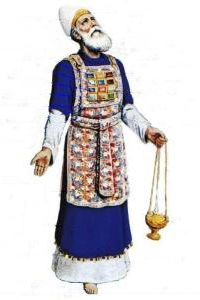
\includegraphics[width=50mm,scale=1.5]{Extras/Melchisedec.jpg}
\vspace{0.4in}  % Create a title for the document and write it in bold font
\LARGE{\textbf{\date}} % Again, do a line break
\linebreak 
% Create a subtitle \large{with Outlines, Statistics, Cross References, and Notes}
\vspace{0.5in}
\begin{flushleft}
\LARGE{Day \#44: Sunday, 13 February 2022 LITE  \\}\vspace{0.25in}
\LARGE{Numbers 10-12 Psalm 44 Proverb 13}
\end{flushleft}
\vspace{0.6in}
\bigskip

\normalsize{Xenia, Oh.\\}
\normalsize{created: \today}
\vspace{1.3in}

\end{flushright}
\end{titlepage}

\newpage 
\tableofcontents\hypertarget{TOC}{}

\hyphenation{A-bim-e-lech bre-thren E-phra-im  Gib-e-o-nites Jer-u-sa-lem through-out Phil-i-stines The-o-phil-us Am-a-le-kites ven-geance Mesh-el-e-mi-ah onan-ism Phar-a-oh thoughts grev-ous-ness Hach-a-liah adul-ter-er Shad-rach}

%%%%%%%%%%%%%%%%% EXTRA COLORS
%%%%%%%%%%%%%%%%% EXTRA COLORS
%%%%%%%%%%%%%%%%% EXTRA COLORS
\definecolor{champagne}{rgb}{0.97,0.91,0.81}
\definecolor{bone}{rgb}{0.89,0.85,0.79}

\definecolor{ForestGreen}{rgb}{0.00,0.29,0.098}
\definecolor{GIVING}{cmyk}{1,0.0,0.72,.1}

\definecolor{MLPE}{cmyk}{1,1,0,.45}
\definecolor{SOCCER}{cmyk}{.77, 0, .42, .49}
\definecolor{PAYBILL}{cmyk}{0,0.83,0.76,0.07}
\definecolor{SERMON}{cmyk}{.14,.9,0,.30} % aka seance \href{http://www.flatuicolorpicker.com/purple-cmyk-color-model/}{seance}
\definecolor{BIBLE}{cmyk}{0,.17,.74,.17}
\definecolor{WORKBLUE}{cmyk}{1, .5, 0, .6}
\definecolor{myOrange}{cmyk}{0, .4, .98, .03}
\definecolor{myTan}{cmyk}{0.0,.07,.17,.10}
\definecolor{myRed}{cmyk}{0,1,1,0}
\definecolor{myWhite}{cmyk}{0,0,0,0}
\definecolor{BLUESoD}{cmyk}{.97,.84,0,.04}
\definecolor{WHITE}{cmyk}{0,0,0,0}
\definecolor{OLDGOLD}{cmyk}{0.05,0.3,1.00,0}
\definecolor{CASTLETON}{cmyk}{1,0,0.31,0.66}
\definecolor{cadmiumgreen}{rgb}{0.0, 0.42, 0.24}
\definecolor{jungle}{rgb}{0.203,0.4882,0.1718}
\definecolor{MYGOLD}{rgb}{1,.84,0}

\definecolor{MYLIGHTGRAY}{rgb}{.85,.85,.85}

\definecolor{codegreen}{rgb}{0,0.6,0}
\definecolor{codegray}{rgb}{0.5,0.5,0.5}
\definecolor{codepurple}{rgb}{0.58,0,0.82}
\definecolor{backcolour}{rgb}{0.95,0.95,0.92}


\mdfdefinestyle{MyFrame}{%
    linecolor=blue,
    outerlinewidth=2pt,
    roundcorner=5pt,
    innertopmargin=\baselineskip,
    innerbottommargin=\baselineskip,
    innerrightmargin=10pt,
    innerleftmargin=10pt,
    backgroundcolor=gray!25!white}


\mdfdefinestyle{MyFrame2}{%
    linecolor=black,
    outerlinewidth=2pt,
    roundcorner=5pt,
    innertopmargin=\baselineskip,
    innerbottommargin=\baselineskip,
    innerrightmargin=10pt,
    innerleftmargin=10pt,
    backgroundcolor=yellow!25!white}


%%%%%
%% for PFTTIS list
%%%%%

%%% And Joseph said unto
\index[PFTTIS]{And Joseph said unto!Genesis!Gen 40:008}
\index[PFTTIS]{And Joseph said unto!Genesis!Gen 40:012}
\index[PFTTIS]{And Joseph said unto!Genesis!Gen 41:025}
\index[PFTTIS]{And Joseph said unto!Genesis!Gen 42:014}
\index[PFTTIS]{And Joseph said unto!Genesis!Gen 42:018}
\index[PFTTIS]{And Joseph said unto!Genesis!Gen 44:015}
\index[PFTTIS]{And Joseph said unto!Genesis!Gen 45:003}
\index[PFTTIS]{And Joseph said unto!Genesis!Gen 45:004}
\index[PFTTIS]{And Joseph said unto!Genesis!Gen 46:031}
\index[PFTTIS]{And Joseph said unto!Genesis!Gen 48:009}
\index[PFTTIS]{And Joseph said unto!Genesis!Gen 48:018}
\index[PFTTIS]{And Joseph said unto!Genesis!Gen 50:019}
\index[PFTTIS]{And Joseph said unto!Genesis!Gen 50:024}


%%% a shadow
\index[PFTTIS]{a shadow!1Chronicles!1Chr 029:15}
\index[PFTTIS]{a shadow!Job!Job 008:09}
\index[PFTTIS]{a shadow!Job!Job 014:02}
\index[PFTTIS]{a shadow!Job!Job 017:07}
\index[PFTTIS]{a shadow!Psalm!Psa 102:011}
\index[PFTTIS]{a shadow!Psalm!Psa 144:004}
\index[PFTTIS]{a shadow!Ecclesiastes!Eccl 006:012}
\index[PFTTIS]{a shadow!Ecclesiastes!Eccl 008:013}
\index[PFTTIS]{a shadow!Isaiah!Isa 04:006}
\index[PFTTIS]{a shadow!Isaiah!Isa 25:004}
\index[PFTTIS]{a shadow!Jonah!Jnh 04:06}
\index[PFTTIS]{a shadow!Colossians!Col 02:017}
\index[PFTTIS]{a shadow!Hebews!Heb 10:001}

%%% blessed is the man
\index[PFTTIS]{blessed is the man!Psalm!Psa 001:001}
\index[PFTTIS]{blessed is the man!Psalm!Psa 032:002}
\index[PFTTIS]{blessed is the man!Psalm!Psa 034:008}
\index[PFTTIS]{blessed is the man!Psalm!Psa 065:004}
\index[PFTTIS]{blessed is the man!Psalm!Psa 084:005}
\index[PFTTIS]{blessed is the man!Psalm!Psa 084:012}
\index[PFTTIS]{blessed is the man!Psalm!Psa 094:012}
\index[PFTTIS]{blessed is the man!Psalm!Psa 112:001}
\index[PFTTIS]{blessed is the man!Proverbs!Pro 008:034}
\index[PFTTIS]{blessed is the man!Isaiah!Isa 056:002}
\index[PFTTIS]{blessed is the man!Jeremiah!Jer 017:007}
\index[PFTTIS]{blessed is the man!Romans!Rom 004:008}
\index[PFTTIS]{blessed is the man!James!Jam 001:012}


%%% carry them
\index[PFTTIS]{carry them!Leviticus!Lev 14:045}
\index[PFTTIS]{carry them!Numbers!Num 11:012}
\index[PFTTIS]{carry them!Joshua!Jsh 04:003}
\index[PFTTIS]{carry them!1Samuel!1Sam 20:040}
\index[PFTTIS]{carry them!1Kings!1Kng 08:046}
\index[PFTTIS]{carry them!2Chronicles!2Chr 06:036}
\index[PFTTIS]{carry them!Ezra!Ezra 05:015}
\index[PFTTIS]{carry them!Isaiah!Isa 40:011}
\index[PFTTIS]{carry them!Isaiah!Isa 41:016}
\index[PFTTIS]{carry them!Isaiah!Isa 57:013}
\index[PFTTIS]{carry them!Jeremiah!Jer 20:004}
\index[PFTTIS]{carry them!Jeremiah!Jer 20:005}
\index[PFTTIS]{carry them!Jeremiah!Jer 43:012}


\index[PFTTIS]{good tidings!2Samuel!2Sam 18:027}
\index[PFTTIS]{good tidings!1Kings!1Ki 01:042}
\index[PFTTIS]{good tidings!2Kings!2Ki 07:009 (2x)}
\index[PFTTIS]{good tidings!Isaiah!Isa 40:009 (2x)}
\index[PFTTIS]{good tidings!Isaiah!Isa 41:007}
\index[PFTTIS]{good tidings!Isaiah!Isa 52:007}
\index[PFTTIS]{good tidings!Isaiah!Isa 61:001}
\index[PFTTIS]{good tidings!Nahum!Nah 01:005}
\index[PFTTIS]{good tidings!Luke!Lk 02:010}
\index[PFTTIS]{good tidings!1Thessalonians!1Thess 03:006}


%%% dead body
\index[PFTTIS]{dead body!Leviticus!Lev 21:011}
\index[PFTTIS]{dead body!Numbers!Num 06:006}
\index[PFTTIS]{dead body!Numbers!Num 09:006}
\index[PFTTIS]{dead body!Numbers!Num 09:007}
\index[PFTTIS]{dead body!Numbers!Num 09:010}
\index[PFTTIS]{dead body!Numbers!Num 09:011}
\index[PFTTIS]{dead body!Numbers!Num 09:013}
\index[PFTTIS]{dead body!Numbers!Num 09:016}
\index[PFTTIS]{dead body!2Kings!2Ki 08:005}
\index[PFTTIS]{dead body!Isaiah!Isa 26:019}
\index[PFTTIS]{dead body!Jeremiah!Jer 26:023}
\index[PFTTIS]{dead body!Jeremiah!Jer 36:030}
\index[PFTTIS]{dead body!Haggai!Hag 02:013}

%%% great sea
\index[PFTTIS]{great sea!Numbers!Num 34:006}
\index[PFTTIS]{great sea!Numbers!Num 34:007}
\index[PFTTIS]{great sea!Joshua!Jos 01:004}
\index[PFTTIS]{great sea!Joshua!Jos 09:001}
\index[PFTTIS]{great sea!Joshua!Jos 15:012}
\index[PFTTIS]{great sea!Joshua!Jos 15:047}
\index[PFTTIS]{great sea!Joshua!Jos 23:004}
\index[PFTTIS]{great sea!Ezekiel!Eze 47:010}
\index[PFTTIS]{great sea!Ezekiel!Eze 47:015}
\index[PFTTIS]{great sea!Ezekiel!Eze 47:019}
\index[PFTTIS]{great sea!Ezekiel!Eze 47:020}
\index[PFTTIS]{great sea!Ezekiel!Eze 48:028}
\index[PFTTIS]{great sea!Daniel!Dan 07:002}


%%% have forsaken me
\index[PFTTIS]{have forsaken me!Judges!Jdg 10:013}
\index[PFTTIS]{have forsaken me!1Samuel!1Sam 08:008}
\index[PFTTIS]{have forsaken me!1Kings!1Ki 11:033}
\index[PFTTIS]{have forsaken me!2Kings!2Ki 22:017}
\index[PFTTIS]{have forsaken me!2Chronicles!2Chr 12:005}
\index[PFTTIS]{have forsaken me!2Chronicles!2Chr 34:025}
\index[PFTTIS]{have forsaken me!Jeremiah!Jer 01:016}
\index[PFTTIS]{have forsaken me!Jeremiah!Jer 02:013}
\index[PFTTIS]{have forsaken me!Jeremiah!Jer 05:007}
\index[PFTTIS]{have forsaken me!Jeremiah!Jer 05:019}
\index[PFTTIS]{have forsaken me!Jeremiah!Jer 16:011 (2x)}
\index[PFTTIS]{have forsaken me!Jeremiah!Jer 19:004}

%%% no king
\index[PFTTIS]{no king!Judges!Jdg 17:06}
\index[PFTTIS]{no king!Judges!Jdg 18:01}
\index[PFTTIS]{no king!Judges!Jdg 19:01}
\index[PFTTIS]{no king!Judges!Jdg 21:25}
\index[PFTTIS]{no king!1Kings!1Ki 22:47}
\index[PFTTIS]{no king!2Kings!2Ki 23:25}
\index[PFTTIS]{no king!Nehemiah!Neh 13:26}
\index[PFTTIS]{no king!Psalms!Psa 033:016}
\index[PFTTIS]{no king!Proverbs!Pro 30:27}
\index[PFTTIS]{no king!Daniel!Dan 02:10}
\index[PFTTIS]{no king!Hosea!Hos 10:03}
\index[PFTTIS]{no king!Micah!Mic 04:09}
\index[PFTTIS]{no king!John!Jhn 19:15}


%%% rebellious house
\index[PFTTIS]{rebellious house!Exodus!Exo 02:005}
\index[PFTTIS]{rebellious house!Exodus!Exo 02:006}
\index[PFTTIS]{rebellious house!Exodus!Exo 02:008}
\index[PFTTIS]{rebellious house!Exodus!Exo 03:009}
\index[PFTTIS]{rebellious house!Exodus!Exo 03:026}
\index[PFTTIS]{rebellious house!Exodus!Exo 03:027}
\index[PFTTIS]{rebellious house!Exodus!Exo 12:002 (2x)}
\index[PFTTIS]{rebellious house!Exodus!Exo 12:003}
\index[PFTTIS]{rebellious house!Exodus!Exo 12:009}
\index[PFTTIS]{rebellious house!Exodus!Exo 12:025}
\index[PFTTIS]{rebellious house!Exodus!Exo 17:012}
\index[PFTTIS]{rebellious house!Exodus!Exo 24:003}

%%% seek him
\index[PFTTIS]{seek him!Deuteronomy!Deu 04:029}\index[PFTTIS]{seek him!1Samuel!1Sam 23:025}
\index[PFTTIS]{seek him!1Chronicles!1Chr 28:009}
\index[PFTTIS]{seek him!2Chronicles!1Chr 15:002}
\index[PFTTIS]{seek him!Ezra!Ezr 08:022}
\index[PFTTIS]{seek him!Psalms!Psa 022:026}
\index[PFTTIS]{seek him!Psalms!Psa 024:006}
\index[PFTTIS]{seek him!Psalms!Psa 119:002}
\index[PFTTIS]{seek him!SoS!SoS 03:002}
\index[PFTTIS]{seek him!SoS!SoS 06:001}
\index[PFTTIS]{seek him!Hosea!Hos 07:010}
\index[PFTTIS]{seek him!Amos!Amo 05:008}
\index[PFTTIS]{seek him!Hebrews!Heb 11:0063}


%%% seek ye
\index[PFTTIS]{seek ye!Isaiah!Isa 34:016}
\index[PFTTIS]{seek ye!Isaiah!Isa 45:019}
\index[PFTTIS]{seek ye!Isaiah!Isa 55:006}
\index[PFTTIS]{seek ye!Amos!Amos 5:004}
\index[PFTTIS]{seek ye!John!John 1:38}
\index[PFTTIS]{seek ye!John!John 18:4}
\index[PFTTIS]{seek ye!John!John 18:7}
\index[PFTTIS]{seek ye!Matthew!Matt 6:33}
\index[PFTTIS]{seek ye!Numbers!Num 16:10}
\index[PFTTIS]{seek ye!Luke!Luke 12:31}
\index[PFTTIS]{seek ye!Luke!Luke 24:5}
\index[PFTTIS]{seek ye!Psalm!Psa 27:8}
\index[PFTTIS]{seek ye!Zephaniah!Zeph 2:3}

%%% the uncircumcised
\index[PFTTIS]{the uncircumcised!Genesis!Gen 17:014}
\index[PFTTIS]{the uncircumcised!Judges!Jdg 14:003}
\index[PFTTIS]{the uncircumcised!Judges!Jdg 15:018}
\index[PFTTIS]{the uncircumcised!2Samuel!2Sam 01:020}
\index[PFTTIS]{the uncircumcised!Isaiah!Isa 02:001}
\index[PFTTIS]{the uncircumcised!Jeremiah!Jer 09:025}
\index[PFTTIS]{the uncircumcised!Ezekiel!Eze 28:010}
\index[PFTTIS]{the uncircumcised!Ezekiel!Eze 31:018}
\index[PFTTIS]{the uncircumcised!Ezekiel!Eze 32:019}
\index[PFTTIS]{the uncircumcised!Ezekiel!Eze 32:027}
\index[PFTTIS]{the uncircumcised!Ezekiel!Eze 32:028}
\index[PFTTIS]{the uncircumcised!Ezekiel!Eze 32:029}
\index[PFTTIS]{the uncircumcised!Ezekiel!Eze 32:032}

%%% worship him
\index[PFTTIS]{worship him!Psalms!Psa 97:007}
\index[PFTTIS]{worship him!Zephaniah!Zeph 02:011}
\index[PFTTIS]{worship him!Matthew!Matt 02:002}
\index[PFTTIS]{worship him!Matthew!Matt 02:008}
\index[PFTTIS]{worship him!John!John 04:023}
\index[PFTTIS]{worship him!John!John 04:024 (2x)} 
\index[PFTTIS]{worship him!Acts!Acts 17:023}
\index[PFTTIS]{worship him!Hebrews!Heb 01:006}
\index[PFTTIS]{worship him!Revelation!Rev 04:010}
\index[PFTTIS]{worship him!Revelation!Rev 13:008}
\index[PFTTIS]{worship him!Revelation!Rev 14:007}
\index[PFTTIS]{worship him!Revelation!Rev 19:010}


%%%%%
%% for PFTTIS list
%%%%%

%%% afflictions
\index[WFTTIS]{afflictions!Psalms!Psa 34:019}
\index[WFTTIS]{afflictions!Psalms!Psa 132:001}
\index[WFTTIS]{afflictions!Acts!Acts 07:010}
\index[WFTTIS]{afflictions!Acts!Acts 20:023}
\index[WFTTIS]{afflictions!2Corinthians!2Cor 06:004}
\index[WFTTIS]{afflictions!Colossians!Col 01:024}
\index[WFTTIS]{afflictions!1Thessalonians!1Thess 03:003}
\index[WFTTIS]{afflictions!2Timothy!2Tim 01:008}
\index[WFTTIS]{afflictions!2Timothy!2Tim 03:011}
\index[WFTTIS]{afflictions!2Timothy!2Tim 04:005}
\index[WFTTIS]{afflictions!Hebrews!Heb 10:032}
\index[WFTTIS]{afflictions!Hebrews!Heb 10:033}
\index[WFTTIS]{afflictions!1Peter!1Pet 05:009}

%%% acsend
\index[WFTTIS]{acsend!Joshua!Jos 06:05}
\index[WFTTIS]{acsend!Psalm!Psa 024:003}
\index[WFTTIS]{acsend!Psalm!Psa 135:007}
\index[WFTTIS]{acsend!Psalm!Psa 139:008}
\index[WFTTIS]{acsend!Isaiah!Isa 14:013}
\index[WFTTIS]{acsend!Isaiah!Isa 14:014}
\index[WFTTIS]{acsend!Jeremiah!Jer 10:013}
\index[WFTTIS]{acsend!Jeremiah!Jer 51:016}
\index[WFTTIS]{acsend!Ezekiel!Eze 38:009}
\index[WFTTIS]{acsend!John!John 06:062}
\index[WFTTIS]{acsend!John!John 20:017}
\index[WFTTIS]{acsend!Romans!Rom 10:006}
\index[WFTTIS]{acsend!Revelation!Rev 17:008}

%%% Assyrian
\index[WFTTIS]{Assyrian!Isaiah!Isa 10:005}
\index[WFTTIS]{Assyrian!Isaiah!Isa 10:024}
\index[WFTTIS]{Assyrian!Isaiah!Isa 14:025}
\index[WFTTIS]{Assyrian!Isaiah!Isa 19:023}
\index[WFTTIS]{Assyrian!Isaiah!Isa 23:013}
\index[WFTTIS]{Assyrian!Isaiah!Isa 30:031}
\index[WFTTIS]{Assyrian!Isaiah!Isa 31:008}
\index[WFTTIS]{Assyrian!Isaiah!Isa 52:004}
\index[WFTTIS]{Assyrian!Ezekiel!Eze 31:003}
\index[WFTTIS]{Assyrian!Hosea!Hos 05:013}
\index[WFTTIS]{Assyrian!Hosea!Hos 11:005}
\index[WFTTIS]{Assyrian!Micah!Hos 05:005}
\index[WFTTIS]{Assyrian!Micah!Hos 05:006}

%%% blot
\index[WFTTIS]{blot!Exodus!Exo 32:032}
\index[WFTTIS]{blot!Exodus!Exo 32:033}
\index[WFTTIS]{blot!Numbers!Num 05:026}
\index[WFTTIS]{blot!Deuteronomy!Deut 09:014}
\index[WFTTIS]{blot!Deuteronomy!Deut 25:019}
\index[WFTTIS]{blot!Deuteronomy!Deut 29:020}
\index[WFTTIS]{blot!2Kings!2Ki 14:027}
\index[WFTTIS]{blot!Job!Job 31:007}
\index[WFTTIS]{blot!Psalms!Psa 51:001}
\index[WFTTIS]{blot!Psalms!Psa 51:009}
\index[WFTTIS]{blot!Proverbs!Pro 09:007}
\index[WFTTIS]{blot!Jeremiah!Jer 18:023}
\index[WFTTIS]{blot!Revelation!Rev 03:005}


%%% chain
\index[WFTTIS]{chain!Genesis!Gen 41:042}
\index[WFTTIS]{chain!1Kings!1Ki 07:017}
\index[WFTTIS]{chain!Psalms!Psa 73:006}
\index[WFTTIS]{chain!SoS!Sos 04:009}
\index[WFTTIS]{chain!Lamentations!Lam 03:007}
\index[WFTTIS]{chain!Ezekiel!Eze 07:023}
\index[WFTTIS]{chain!Ezekiel!Eze 16:011}
\index[WFTTIS]{chain!Daniel!Dan 05:007}
\index[WFTTIS]{chain!Daniel!Dan 05:016}
\index[WFTTIS]{chain!Daniel!Dan 05:029}
\index[WFTTIS]{chain!Acts!Acts 28:020}
\index[WFTTIS]{chain!2Timothy!2Tim 01:016}
\index[WFTTIS]{chain!Revelation!Rev 20:001}


%%% controversy
\index[WFTTIS]{controversy!Deuteronomy!Deu 17:008}
\index[WFTTIS]{controversy!Deuteronomy!Deu 19:017}
\index[WFTTIS]{controversy!Deuteronomy!Deu 21:005}
\index[WFTTIS]{controversy!Deuteronomy!Deu 25:001}
\index[WFTTIS]{controversy!2Samuel!2Sam 15:002}
\index[WFTTIS]{controversy!Isaiah!Isa 34:008}
\index[WFTTIS]{controversy!Jeremiah!Jer 25:031}
\index[WFTTIS]{controversy!Ezekiel!Eze 44:024}
\index[WFTTIS]{controversy!Hosea!Hos 04:001}
\index[WFTTIS]{controversy!Hosea!Hos 12:002}
\index[WFTTIS]{controversy!Micah!Mic 06:002 (2x)}
\index[WFTTIS]{controversy!1Timothy!1Tim 03:016}


%%% Dagon/Dagon's
\index[WFTTIS]{Dagon!Judges!Jdg 16:023}
\index[WFTTIS]{Dagon!1Samuel!1Sam 05:002 (2x)}
\index[WFTTIS]{Dagon!1Samuel!1Sam 05:003 (2x)}
\index[WFTTIS]{Dagon!1Samuel!1Sam 05:004 (3x)}
\index[WFTTIS]{Dagon!1Samuel!1Sam 05:005 (3x)}
\index[WFTTIS]{Dagon!1Samuel!1Sam 05:007}
\index[WFTTIS]{Dagon!1Chronicles!1Chr 10:010}

%%% disobedient
\index[WFTTIS]{disobedient!1Kings!1Ki 13:026}
\index[WFTTIS]{disobedient!Nehemiah!Neh 09:026}
\index[WFTTIS]{disobedient!Luke!Luke 01:017}
\index[WFTTIS]{disobedient!Acts!Acts 26:019}
\index[WFTTIS]{disobedient!Romans!Rom 01:030}
\index[WFTTIS]{disobedient!Romans!Rom 10:021}
\index[WFTTIS]{disobedient!1Timothy!1Tim 01:009}
\index[WFTTIS]{disobedient!2Timothy!2Tim 03:002}
\index[WFTTIS]{disobedient!Titus!Titus 01:016}
\index[WFTTIS]{disobedient!Titus!Titus 03:003}
\index[WFTTIS]{disobedient!1Peter!1Pet 02:007}
\index[WFTTIS]{disobedient!1Peter!1Pet 02:008}
\index[WFTTIS]{disobedient!1Peter!1Pet 03:020}


%%% doubt
\index[WFTTIS]{doubt!Genesis!Gen 37:033}
\index[WFTTIS]{doubt!Deuteronomy!Deu 28:066}
\index[WFTTIS]{doubt!Job!Job 12:002}
\index[WFTTIS]{doubt!Matthew!Matt 14:031}
\index[WFTTIS]{doubt!Matthew!Matt 21:021}
\index[WFTTIS]{doubt!Mark!Mk 11:023}
\index[WFTTIS]{doubt!Luke!Lk 11:020}
\index[WFTTIS]{doubt!John!Jhn 10:024}
\index[WFTTIS]{doubt!Acts!Acts 02:012}
\index[WFTTIS]{doubt!Acts!Acts 28:004}
\index[WFTTIS]{doubt!1Corinthians!1Cor 09:010}
\index[WFTTIS]{doubt!Galatians!Gal 04:020}
\index[WFTTIS]{doubt!1John!1Jhn 02:019}


%%% dungeon
\index[WFTTIS]{dungeon!Genesis!Gen 40:015}
\index[WFTTIS]{dungeon!Genesis!Gen 41:014}
\index[WFTTIS]{dungeon!Exodus!Exo 12:029}
\index[WFTTIS]{dungeon!Jeremiah!Jer 37:016}
\index[WFTTIS]{dungeon!Jeremiah!Jer 38:006 (2x)}
\index[WFTTIS]{dungeon!Jeremiah!Jer 38:007}
\index[WFTTIS]{dungeon!Jeremiah!Jer 38:009}
\index[WFTTIS]{dungeon!Jeremiah!Jer 38:010}
\index[WFTTIS]{dungeon!Jeremiah!Jer 38:011}
\index[WFTTIS]{dungeon!Jeremiah!Jer 38:013}
\index[WFTTIS]{dungeon!Lamentations!Lam 03:053}
\index[WFTTIS]{dungeon!Lamentations!Lam 03:055}


%%% error
\index[WFTTIS]{error!2Samuel!2Sam 06:007}
\index[WFTTIS]{error!Job!Job 19:004}
\index[WFTTIS]{error!Ecclesiastes!Ecc 05:006}
\index[WFTTIS]{error!Ecclesiastes!Ecc 10:005}
\index[WFTTIS]{error!Isaiah!Isa 32:006}
\index[WFTTIS]{error!Daniel!Dan 06:004}
\index[WFTTIS]{error!Matthew!Matt 27:064}
\index[WFTTIS]{error!Romans!Rom 01:027}
\index[WFTTIS]{error!James!Jam 05:020}
\index[WFTTIS]{error!2Peter!2Pet 02:018}
\index[WFTTIS]{error!2Peter!2Pet 03:017}
\index[WFTTIS]{error!1John!1Jn 04:006}
\index[WFTTIS]{error!Jude!Jude 01:011}

%%% fourish
\index[WFTTIS]{fourish!Psalms!Psa 072:007}
\index[WFTTIS]{fourish!Psalms!Psa 072:016}
\index[WFTTIS]{fourish!Psalms!Psa 092:007}
\index[WFTTIS]{fourish!Psalms!Psa 092:012}
\index[WFTTIS]{fourish!Psalms!Psa 092:013}
\index[WFTTIS]{fourish!Psalms!Psa 132:018}
\index[WFTTIS]{fourish!Proverbs!Pro 11:28}
\index[WFTTIS]{fourish!Proverbs!Pro 14:11}
\index[WFTTIS]{fourish!Ecclesiastes!Ecc 12:05}
\index[WFTTIS]{fourish!SongOfSolomon!SOS 07:12}
\index[WFTTIS]{fourish!Isaiah!Isa 17:11}
\index[WFTTIS]{fourish!Isaiah!Isa 66:14}
\index[WFTTIS]{fourish!Ezekiel!Eze 17:24}




%%% giants
\index[WFTTIS]{giants!Genesis!Gen 06:004}
\index[WFTTIS]{giants!Numbers!Num 13:033}
\index[WFTTIS]{giants!Deuteronomy!Deut 02:011}
\index[WFTTIS]{giants!Deuteronomy!Deut 02:021}
\index[WFTTIS]{giants!Deuteronomy!Deut 03:011}
\index[WFTTIS]{giants!Deuteronomy!Deut 03:013}
\index[WFTTIS]{giants!Joshua!Josh 12:004}
\index[WFTTIS]{giants!Joshua!Josh 13:012}
\index[WFTTIS]{giants!Joshua!Josh 15:008}
\index[WFTTIS]{giants!Joshua!Josh 17:015}
\index[WFTTIS]{giants!Joshua!Josh 16:016}

%%% good man
\index[WFTTIS]{good man!2 Samuel!2Sa 18:27}
%(1) Psalms 37:23 [5]
%(1) Psalms 112:5 [2]
%(1) Proverbs 12:2 [2]
%(1) Proverbs 13:22 [2]
%(1) Proverbs 14:14 [14]
%(1) Micah 7:2 [2]
%(1) Matthew 12:35 [2]
%(1) Luke 6:45 [2]
%(1) Luke 23:50 [15]
%(1) John 7:12 [17]
%(1) Acts 11:24 [5]
%(1) Romans 5:7 [14]

%%% Hinnom
\index[WFTTIS]{Hinnom!Joshua!Jsh 15:008}
\index[WFTTIS]{Hinnom!Joshua!Jsh 18:016}
\index[WFTTIS]{Hinnom!2Kings!2Ki 23:010}
\index[WFTTIS]{Hinnom!2Chronicles!2Chr 28:003}
\index[WFTTIS]{Hinnom!2Chronicles!2Chr 33:006}
\index[WFTTIS]{Hinnom!Nehemiah!Neh 11:030}
\index[WFTTIS]{Hinnom!Jeremiah!Jer 07:031}
\index[WFTTIS]{Hinnom!Jeremiah!Jer 07:032}
\index[WFTTIS]{Hinnom!Jeremiah!Jer 19:002}
\index[WFTTIS]{Hinnom!Jeremiah!Jer 19:006}
\index[WFTTIS]{Hinnom!Jeremiah!Jer 32:035}

%%% inclined
\index[WFTTIS]{inclined!Judges!Jdg 09:003}
\index[WFTTIS]{inclined!Psalms!Psa 040:001}
\index[WFTTIS]{inclined!Psalms!Psa 116:002}
\index[WFTTIS]{inclined!Psalms!Psa 119:112}
\index[WFTTIS]{inclined!Proverbs!Pro 05:13}
\index[WFTTIS]{inclined!Jeremiah!Jer 07:24}
\index[WFTTIS]{inclined!Jeremiah!Jer 07:26}
\index[WFTTIS]{inclined!Jeremiah!Jer 11:08}
\index[WFTTIS]{inclined!Jeremiah!Jer 17:23}
\index[WFTTIS]{inclined!Jeremiah!Jer 25:04}
\index[WFTTIS]{inclined!Jeremiah!Jer 34:14}
\index[WFTTIS]{inclined!Jeremiah!Jer 35:15}
\index[WFTTIS]{inclined!Jeremiah!Jer 44:05}


%%% laughed
\index[WFTTIS]{laughed!Genesis!Gen 17:017}
\index[WFTTIS]{laughed!Genesis!Gen 18:012}
\index[WFTTIS]{laughed!Genesis!Gen 18:015}
\index[WFTTIS]{laughed!2Kings!2Ki 19:021}
\index[WFTTIS]{laughed!2Chronicles!2Chr 30:010}
\index[WFTTIS]{laughed!Nehemiah!Neh 02:019}
\index[WFTTIS]{laughed!Job!Job 12:004}
\index[WFTTIS]{laughed!Job!Job 29:024}
\index[WFTTIS]{laughed!Isaiah!Isa 37:022}
\index[WFTTIS]{laughed!Ezekiel!Ezek 23:032}
\index[WFTTIS]{laughed!Matthew!Matt 09:024}
\index[WFTTIS]{laughed!Mark!Mk 05:040}
\index[WFTTIS]{laughed!Luke!Lk 08:053}

%%% liar
\index[WFTTIS]{liar!Job!Job 24:025}
\index[WFTTIS]{liar!Proverbs!Pro 17:004}
\index[WFTTIS]{liar!Proverbs!Pro 19:022}
\index[WFTTIS]{liar!Proverbs!Pro 30:006}
\index[WFTTIS]{liar!Jeremiah!Jer 15:018}
\index[WFTTIS]{liar!John!Jhn 08:044}
\index[WFTTIS]{liar!John!Jhn 08:055}
\index[WFTTIS]{liar!Romans!Rom 03:004}
\index[WFTTIS]{liar!1John!1Jhn 01:010}
\index[WFTTIS]{liar!1John!1Jhn 02:004}
\index[WFTTIS]{liar!1John!1Jhn 02:022}
\index[WFTTIS]{liar!1John!1Jhn 04:020}
\index[WFTTIS]{liar!1John!1Jhn 05:010}

%%% palsy
\index[WFTTIS]{palsy!Matthew!Matt 04:024}
\index[WFTTIS]{palsy!Matthew!Matt 08:006}
\index[WFTTIS]{palsy!Matthew!Matt 09:002}
\index[WFTTIS]{palsy!Matthew!Matt 09:006}
\index[WFTTIS]{palsy!Mark!Mk 02:003}
\index[WFTTIS]{palsy!Mark!Mk 02:004}
\index[WFTTIS]{palsy!Mark!Mk 02:005}
\index[WFTTIS]{palsy!Mark!Mk 02:009}
\index[WFTTIS]{palsy!Mark!Mk 02:010}
\index[WFTTIS]{palsy!Luke!Lk 05:018}
\index[WFTTIS]{palsy!Luke!Lk 05:024}
\index[WFTTIS]{palsy!Acts!Acts 09:033}

%%% Profitable
\index[WFTTIS]{profitable!Job!Job 22:002 (2x)}
\index[WFTTIS]{profitable!Ecclesiastes!Ecc 10:010}
\index[WFTTIS]{profitable!Isaiah!Isa 44:010}
\index[WFTTIS]{profitable!Jeremiah!Jer 13:007}
\index[WFTTIS]{profitable!Matthew!Matt 05:029}
\index[WFTTIS]{profitable!Matthew!Matt 05:030}
\index[WFTTIS]{profitable!Acts!Acts 20:020}
\index[WFTTIS]{profitable!1Timothy!1Tim 04:008}
\index[WFTTIS]{profitable!2Timothy!2Tim 03:016}
\index[WFTTIS]{profitable!2Timothy!2Tim 04:011}
\index[WFTTIS]{profitable!Titus!Titus 03:008}
\index[WFTTIS]{profitable!Philemon!Phlm 01:011}

%%% Rechab
\index[WFTTIS]{Rechab!2Samuel!2Sam 04:002}
\index[WFTTIS]{Rechab!2Samuel!2Sam 04:005}
\index[WFTTIS]{Rechab!2Samuel!2Sam 04:006}
\index[WFTTIS]{Rechab!2Samuel!2Sam 04:009}
\index[WFTTIS]{Rechab!2KIngs!2Ki 10:015}
\index[WFTTIS]{Rechab!2KIngs!2Ki 10:023}
\index[WFTTIS]{Rechab!1Chronicles!1Chr 02:055}
\index[WFTTIS]{Rechab!Nehemiah!Neh 03:014}
\index[WFTTIS]{Rechab!Jeremiah!Jer 35:006}
\index[WFTTIS]{Rechab!Jeremiah!Jer 35:008}
\index[WFTTIS]{Rechab!Jeremiah!Jer 35:014}
\index[WFTTIS]{Rechab!Jeremiah!Jer 35:016}
\index[WFTTIS]{Rechab!Jeremiah!Jer 35:019}

%%% serpents
\index[WFTTIS]{serpents!Exodus!Exo 07:012}
\index[WFTTIS]{serpents!Numbers!Num 21:006}
\index[WFTTIS]{serpents!Numbers!Num 21:007}
\index[WFTTIS]{serpents!Deuteronomy!Deu 08:015}
\index[WFTTIS]{serpents!Deuteronomy!Deu 32:024}
\index[WFTTIS]{serpents!Jeremiah!Jer 08:017}
\index[WFTTIS]{serpents!Matthew!Matt 10:016}
\index[WFTTIS]{serpents!Matthew!Matt 23:033}
\index[WFTTIS]{serpents!Mark!Mk 16:018}
\index[WFTTIS]{serpents!Luke!Lk 10:019}
\index[WFTTIS]{serpents!1Corinthians!1Cor 10:009}
\index[WFTTIS]{serpents!James!Jas 03:007}
\index[WFTTIS]{serpents!Revelation!Rev 09:019}

%%% short
\index[WFTTIS]{short!Numbers!Num 11:023}
\index[WFTTIS]{short!2Kings!2Ki 10:032}
\index[WFTTIS]{short!Job!Job 17:012}
\index[WFTTIS]{short!Job!Job 20:005}
\index[WFTTIS]{short!Psalms!Psa 89:047}
\index[WFTTIS]{short!Romans!Rom 03:023}
\index[WFTTIS]{short!Romans!Rom 09:028  (2x)}
\index[WFTTIS]{short!1Corinthians!1Cor 07:029}
\index[WFTTIS]{short!1Thessalonians!1Thess 02:017}
\index[WFTTIS]{short!Hebrews!Heb 04:001}
\index[WFTTIS]{short!Revelation!Rev 12:012}
\index[WFTTIS]{short!Revelation!Rev 17:010}

%%% smiteth
\index[WFTTIS]{smiteth!Exodus!Exo 21:012}
\index[WFTTIS]{smiteth!Exodus!Exo 21:15}
\index[WFTTIS]{smiteth!Deuteronomy!Dt 25:11}
\index[WFTTIS]{smiteth!Deuteronomy!Dt 27:24}
\index[WFTTIS]{smiteth!Joshua!Jsh 15:16}
\index[WFTTIS]{smiteth!Judges!Jdg 15:16}
\index[WFTTIS]{smiteth!2 Samuel!2Sa 05:08}
\index[WFTTIS]{smiteth!1Chronicles!1Chr 11:06}
\index[WFTTIS]{smiteth!Job!1Chr 26:12}
\index[WFTTIS]{smiteth!Isaiah!Isa 09:13}
\index[WFTTIS]{smiteth!Lamentations!Lam 03:30}
\index[WFTTIS]{smiteth!Ezekiel!Eze 07:09}
\index[WFTTIS]{smiteth!Luke!Lk 06:29}



%%% vanities
\index[WFTTIS]{vanities!Deuteronomy!Deut 21:021}
\index[WFTTIS]{vanities!1Kings!1Ki 16:013}
\index[WFTTIS]{vanities!1Kings!1Ki 16:026}
\index[WFTTIS]{vanities!Psalms!Psa 031:006}
\index[WFTTIS]{vanities!Ecclesiastes!Ecc 01:002 (2x)}
\index[WFTTIS]{vanities!Ecclesiastes!Ecc 05:007}
\index[WFTTIS]{vanities!Ecclesiastes!Ecc 12:008}
\index[WFTTIS]{vanities!Jeremiah!Jer 08:019}
\index[WFTTIS]{vanities!Jeremiah!Jer 10:008}
\index[WFTTIS]{vanities!Jeremiah!Jer 14:022}
\index[WFTTIS]{vanities!Jonah!Jnh 02:008}
\index[WFTTIS]{vanities!Acts!Acts 14:015}



%%%%%
%% for PFTTIS list
%%%%%

%%% worm
\index[WFITV]{worm!Exodus!Exo 16:024}
\index[WFITV]{worm!Job!Job 17:014}
\index[WFITV]{worm!Job!Job 24:029}
\index[WFITV]{worm!Job!Job 25:005 (2x)}
\index[WFITV]{worm!Psalms!Psa 022:006}
\index[WFITV]{worm!Isaiah!Isa 14:011}
\index[WFITV]{worm!Isaiah!Isa 41:014}
\index[WFITV]{worm!Isaiah!Isa 51:008}
\index[WFITV]{worm!Isaiah!Isa 66:024}
\index[WFITV]{worm!Jonah!Jnh 04:007}
\index[WFITV]{worm!Mark!Mk 09:044}
\index[WFITV]{worm!Mark!Mk 09:046}
\index[WFITV]{worm!Mark!Mk 09:048}


%\subsubsection{Title}
%\textbf{Introduction:} Isaiah 46 
%\index[speaker]{Speaker!Isaiah 49 (Title}
%\index[series]{Book (Speaker)!IPassage (Title)}
%\index[date]{2017/07/09!Isaiah 49 (Title)}
%\begin{compactenum}[I.]
%    \item  \textbf{Point} \index[scripture]{Isaiah!IPassage} (IPassage)
%\end{compactenum}




  


\chapter{Numbers 10}

\begin{figure}
  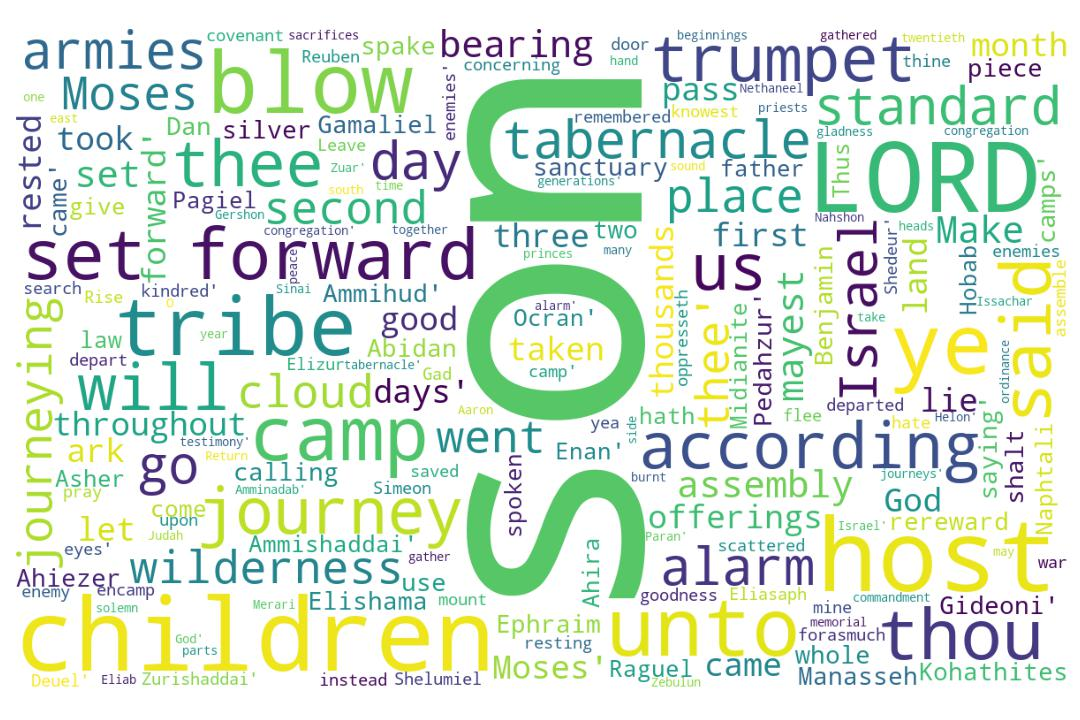
\includegraphics[width=\linewidth]{04OT-Numbers/Numbers10-WordCloud.jpg}
  \caption{Numbers 10 Word Cloud}
  \label{fig:Numbers 10 word Cloud}
\end{figure}


\marginpar{\scriptsize \centering \fcolorbox{bone}{lime}{\textbf{ASSEMBLED}}\\ (Numbers 10:1-36) \begin{compactenum}[I.][8]
    \item An \textbf{Order of Assembly} %\index[scripture]{Psalms!Psalm 044:01}(Psalm 44:1)
    \item An \textbf{Organized Arrangement}  %\index[scripture]{Exodus!Exodus 01:08}(Exodus 1:8)
    \item An \textbf{Obvious Allegory}  (from above, the camp would appear as a cross, with the Tabernacle in the exact middle)%\index[scripture]{Exodus!Exodus 01:08}(Exodus 1:8)
    \item \textbf{Orderly Activity}  %\index[scripture]{Exodus!Exodus 01:08}(Exodus 1:8)
    \item An \textbf{Offer made Available}  \index[scripture]{Numbers!Num 10:29} (Numbers 10:29)
    \item An \textbf{Observed Ark}  (they were to be attentive to the movement, intent, and direction of the Lord) \index[scripture]{Numbers!Num 10:33} (Numbers 10:33)
    \item The \textbf{Opportunity Added-to}  \index[scripture]{Numbers!Num 10:31--32} (Numbers 10:31--32)
\end{compactenum}}



\footnote{\textcolor[cmyk]{0.99998,1,0,0}{\hyperlink{TOC}{Return to end of Table of Contents.}}}\footnote{\href{https://audiobible.com/bible/numbers_10.html}{\textcolor[cmyk]{0.99998,1,0,0}{Numbers 10 Audio}}}\textcolor[cmyk]{0.99998,1,0,0}{And the LORD spake unto Moses, saying,}
[2] \textcolor[cmyk]{0.99998,1,0,0}{Make thee two trumpets of silver; of a whole piece shalt thou make them: that thou mayest use them for the calling of the assembly, and for the journeying of the camps.}
[3] \textcolor[cmyk]{0.99998,1,0,0}{And when they shall blow with them, all the assembly shall assemble themselves to thee at the door of the tabernacle of the congregation.}
[4] \textcolor[cmyk]{0.99998,1,0,0}{And if they blow \emph{but} with one \emph{trumpet}, then the princes, \emph{which} \emph{are} heads of the thousands of Israel, shall gather themselves unto thee.}
[5] \textcolor[cmyk]{0.99998,1,0,0}{When ye blow an alarm, then the camps that lie on the east parts shall go forward.}
[6] \textcolor[cmyk]{0.99998,1,0,0}{When ye blow an alarm the second time, then the camps that lie on the south side shall take their journey: they shall blow an alarm for their journeys.}
[7] \textcolor[cmyk]{0.99998,1,0,0}{But when the congregation is to be gathered together, ye shall blow, but ye shall not sound an alarm.}
[8] \textcolor[cmyk]{0.99998,1,0,0}{And the sons of Aaron, the priests, shall blow with the trumpets; and they shall be to you for an ordinance for ever throughout your generations.}
[9] \textcolor[cmyk]{0.99998,1,0,0}{And if ye go to war in your land against the enemy that oppresseth you, then ye shall blow an alarm with the trumpets; and ye shall be remembered before the LORD your God, and ye shall be saved from your enemies.}
[10] \textcolor[cmyk]{0.99998,1,0,0}{Also in the day of your gladness, and in your solemn days, and in the beginnings of your months, ye shall blow with the trumpets over your burnt offerings, and over the sacrifices of your peace offerings; that they may be to you for a memorial before your God: I \emph{am} the LORD your God.}\\
\\
\P \textcolor[cmyk]{0.99998,1,0,0}{And it came to pass on the twentieth \emph{day} of the second month, in the second year, that the cloud was taken up from off the tabernacle of the testimony.}
[12] \textcolor[cmyk]{0.99998,1,0,0}{And the \fcolorbox{bone}{bone}{children} of Israel took their journeys out of the wilderness of Sinai; and the cloud rested in the wilderness of Paran.}
[13] \textcolor[cmyk]{0.99998,1,0,0}{And they first took their journey according to the commandment of the LORD by the hand of Moses.}
[14] \textcolor[cmyk]{0.99998,1,0,0}{In the first \emph{place} went the standard of the camp of the \fcolorbox{bone}{bone}{children} of Judah according to their armies: and over his host \emph{was} Nahshon the \fcolorbox{bone}{bone}{son} of Amminadab.}
[15] \textcolor[cmyk]{0.99998,1,0,0}{And over the host of the tribe of the \fcolorbox{bone}{bone}{children} of Issachar \emph{was} Nethaneel the \fcolorbox{bone}{bone}{son} of Zuar.}
[16] \textcolor[cmyk]{0.99998,1,0,0}{And over the host of the tribe of the \fcolorbox{bone}{bone}{children} of Zebulun \emph{was} Eliab the \fcolorbox{bone}{bone}{son} of Helon.}
[17] \textcolor[cmyk]{0.99998,1,0,0}{And the tabernacle was taken down; and the sons of Gershon and the sons of Merari set forward, bearing the tabernacle.}\\
\\
\P \textcolor[cmyk]{0.99998,1,0,0}{And the standard of the camp of Reuben set forward according to their armies: and over his host \emph{was} Elizur the \fcolorbox{bone}{bone}{son} of Shedeur.}
[19] \textcolor[cmyk]{0.99998,1,0,0}{And over the host of the tribe of the \fcolorbox{bone}{bone}{children} of Simeon \emph{was} Shelumiel the \fcolorbox{bone}{bone}{son} of Zurishaddai.}
[20] \textcolor[cmyk]{0.99998,1,0,0}{And over the host of the tribe of the \fcolorbox{bone}{bone}{children} of Gad \emph{was} Eliasaph the \fcolorbox{bone}{bone}{son} of Deuel.}
[21] \textcolor[cmyk]{0.99998,1,0,0}{And the Kohathites set forward, bearing the sanctuary: and \emph{the} \emph{other} did set up the tabernacle against they came.}\\
\\
\P \textcolor[cmyk]{0.99998,1,0,0}{And the standard of the camp of the \fcolorbox{bone}{bone}{children} of Ephraim set forward according to their armies: and over his host \emph{was} Elishama the \fcolorbox{bone}{bone}{son} of Ammihud.}
[23] \textcolor[cmyk]{0.99998,1,0,0}{And over the host of the tribe of the \fcolorbox{bone}{bone}{children} of Manasseh \emph{was} Gamaliel the \fcolorbox{bone}{bone}{son} of Pedahzur.}
[24] \textcolor[cmyk]{0.99998,1,0,0}{And over the host of the tribe of the \fcolorbox{bone}{bone}{children} of Benjamin \emph{was} Abidan the \fcolorbox{bone}{bone}{son} of Gideoni.}\\
\\
\P \textcolor[cmyk]{0.99998,1,0,0}{And the standard of the camp of the \fcolorbox{bone}{bone}{children} of Dan set forward, \emph{which} \emph{was} the rereward of all the camps throughout their hosts: and over his host \emph{was} Ahiezer the \fcolorbox{bone}{bone}{son} of Ammishaddai.}
[26] \textcolor[cmyk]{0.99998,1,0,0}{And over the host of the tribe of the \fcolorbox{bone}{bone}{children} of Asher \emph{was} Pagiel the \fcolorbox{bone}{bone}{son} of Ocran.}
[27] \textcolor[cmyk]{0.99998,1,0,0}{And over the host of the tribe of the \fcolorbox{bone}{bone}{children} of Naphtali \emph{was} Ahira the \fcolorbox{bone}{bone}{son} of Enan.}
[28] \textcolor[cmyk]{0.99998,1,0,0}{Thus \emph{were} the journeyings of the \fcolorbox{bone}{bone}{children} of Israel according to their armies, when they set forward.}\\
\\
\P \textcolor[cmyk]{0.99998,1,0,0}{And Moses said unto Hobab, the \fcolorbox{bone}{bone}{son} of Raguel the Midianite, Moses' father in law, We are journeying unto the place of which the LORD said, I will give it you: come thou with us, and we will do thee good: for the LORD hath spoken good concerning Israel.}
[30] \textcolor[cmyk]{0.99998,1,0,0}{And he said unto him, I will not go; but I will depart to mine own land, and to my kindred.}
[31] \textcolor[cmyk]{0.99998,1,0,0}{And he said, Leave us not, I pray thee; forasmuch as thou knowest how we are to encamp in the wilderness, and thou mayest be to us instead of eyes.}
[32] \textcolor[cmyk]{0.99998,1,0,0}{And it shall be, if thou go with us, yea, it shall be, that what goodness the LORD shall do unto us, the same will we do unto thee.}\\
\\
\P \textcolor[cmyk]{0.99998,1,0,0}{And they departed from the mount of the LORD three days' journey: and the ark of the covenant of the LORD went before them in the three days' journey, to search out a resting place for them.}
[34] \textcolor[cmyk]{0.99998,1,0,0}{And the cloud of the LORD \emph{was} upon them by day, when they went out of the camp.}
[35] \textcolor[cmyk]{0.99998,1,0,0}{And it came to pass, when the ark set forward, that Moses said, Rise up, LORD, and let thine enemies be scattered; and let them that hate thee flee before thee.}
[36] \textcolor[cmyk]{0.99998,1,0,0}{And when it rested, he said, Return, O LORD, unto the many thousands of Israel.}
\index[NWIV]{7!Numbers!Num 10:1}\index[AWIP]{And!Numbers!Num 10:1}\index[AWIP]{the!Numbers!Num 10:1}\index[AWIP]{LORD!Numbers!Num 10:1}\index[AWIP]{spake!Numbers!Num 10:1}\index[AWIP]{unto!Numbers!Num 10:1}\index[AWIP]{Moses!Numbers!Num 10:1}\index[AWIP]{saying!Numbers!Num 10:1}

\index[NWIV]{32!Numbers!Num 10:2}\index[AWIP]{Make!Numbers!Num 10:2}\index[AWIP]{thee!Numbers!Num 10:2}\index[AWIP]{two!Numbers!Num 10:2}\index[AWIP]{trumpets!Numbers!Num 10:2}\index[AWIP]{of!Numbers!Num 10:2}\index[AWIP]{of!Numbers!Num 10:2 (2)}\index[AWIP]{of!Numbers!Num 10:2 (3)}\index[AWIP]{of!Numbers!Num 10:2 (4)}\index[AWIP]{silver!Numbers!Num 10:2}\index[AWIP]{a!Numbers!Num 10:2}\index[AWIP]{whole!Numbers!Num 10:2}\index[AWIP]{piece!Numbers!Num 10:2}\index[AWIP]{shalt!Numbers!Num 10:2}\index[AWIP]{thou!Numbers!Num 10:2}\index[AWIP]{thou!Numbers!Num 10:2 (2)}\index[AWIP]{make!Numbers!Num 10:2}\index[AWIP]{them!Numbers!Num 10:2}\index[AWIP]{them!Numbers!Num 10:2 (2)}\index[AWIP]{that!Numbers!Num 10:2}\index[AWIP]{mayest!Numbers!Num 10:2}\index[AWIP]{use!Numbers!Num 10:2}\index[AWIP]{for!Numbers!Num 10:2}\index[AWIP]{for!Numbers!Num 10:2 (2)}\index[AWIP]{the!Numbers!Num 10:2}\index[AWIP]{the!Numbers!Num 10:2 (2)}\index[AWIP]{the!Numbers!Num 10:2 (3)}\index[AWIP]{the!Numbers!Num 10:2 (4)}\index[AWIP]{calling!Numbers!Num 10:2}\index[AWIP]{assembly!Numbers!Num 10:2}\index[AWIP]{and!Numbers!Num 10:2}\index[AWIP]{journeying!Numbers!Num 10:2}\index[AWIP]{camps!Numbers!Num 10:2}

\index[NWIV]{24!Numbers!Num 10:3}\index[AWIP]{And!Numbers!Num 10:3}\index[AWIP]{when!Numbers!Num 10:3}\index[AWIP]{they!Numbers!Num 10:3}\index[AWIP]{shall!Numbers!Num 10:3}\index[AWIP]{shall!Numbers!Num 10:3 (2)}\index[AWIP]{blow!Numbers!Num 10:3}\index[AWIP]{with!Numbers!Num 10:3}\index[AWIP]{them!Numbers!Num 10:3}\index[AWIP]{all!Numbers!Num 10:3}\index[AWIP]{the!Numbers!Num 10:3}\index[AWIP]{the!Numbers!Num 10:3 (2)}\index[AWIP]{the!Numbers!Num 10:3 (3)}\index[AWIP]{the!Numbers!Num 10:3 (4)}\index[AWIP]{assembly!Numbers!Num 10:3}\index[AWIP]{assemble!Numbers!Num 10:3}\index[AWIP]{themselves!Numbers!Num 10:3}\index[AWIP]{to!Numbers!Num 10:3}\index[AWIP]{thee!Numbers!Num 10:3}\index[AWIP]{at!Numbers!Num 10:3}\index[AWIP]{door!Numbers!Num 10:3}\index[AWIP]{of!Numbers!Num 10:3}\index[AWIP]{of!Numbers!Num 10:3 (2)}\index[AWIP]{tabernacle!Numbers!Num 10:3}\index[AWIP]{congregation!Numbers!Num 10:3}

\index[NWIV]{24!Numbers!Num 10:4}\index[AWIP]{And!Numbers!Num 10:4}\index[AWIP]{if!Numbers!Num 10:4}\index[AWIP]{they!Numbers!Num 10:4}\index[AWIP]{blow!Numbers!Num 10:4}\index[AWIP]{\emph{but}!Numbers!Num 10:4}\index[AWIP]{with!Numbers!Num 10:4}\index[AWIP]{one!Numbers!Num 10:4}\index[AWIP]{\emph{trumpet}!Numbers!Num 10:4}\index[AWIP]{then!Numbers!Num 10:4}\index[AWIP]{the!Numbers!Num 10:4}\index[AWIP]{the!Numbers!Num 10:4 (2)}\index[AWIP]{princes!Numbers!Num 10:4}\index[AWIP]{\emph{which}!Numbers!Num 10:4}\index[AWIP]{\emph{are}!Numbers!Num 10:4}\index[AWIP]{heads!Numbers!Num 10:4}\index[AWIP]{of!Numbers!Num 10:4}\index[AWIP]{of!Numbers!Num 10:4 (2)}\index[AWIP]{thousands!Numbers!Num 10:4}\index[AWIP]{Israel!Numbers!Num 10:4}\index[AWIP]{shall!Numbers!Num 10:4}\index[AWIP]{gather!Numbers!Num 10:4}\index[AWIP]{themselves!Numbers!Num 10:4}\index[AWIP]{unto!Numbers!Num 10:4}\index[AWIP]{thee!Numbers!Num 10:4}\index[AWIP]{\emph{but}!Numbers!Num 10:4}\index[AWIP]{\emph{trumpet}!Numbers!Num 10:4}\index[AWIP]{\emph{which}!Numbers!Num 10:4}\index[AWIP]{\emph{are}!Numbers!Num 10:4}

\index[NWIV]{17!Numbers!Num 10:5}\index[AWIP]{When!Numbers!Num 10:5}\index[AWIP]{ye!Numbers!Num 10:5}\index[AWIP]{blow!Numbers!Num 10:5}\index[AWIP]{an!Numbers!Num 10:5}\index[AWIP]{alarm!Numbers!Num 10:5}\index[AWIP]{then!Numbers!Num 10:5}\index[AWIP]{the!Numbers!Num 10:5}\index[AWIP]{the!Numbers!Num 10:5 (2)}\index[AWIP]{camps!Numbers!Num 10:5}\index[AWIP]{that!Numbers!Num 10:5}\index[AWIP]{lie!Numbers!Num 10:5}\index[AWIP]{on!Numbers!Num 10:5}\index[AWIP]{east!Numbers!Num 10:5}\index[AWIP]{parts!Numbers!Num 10:5}\index[AWIP]{shall!Numbers!Num 10:5}\index[AWIP]{go!Numbers!Num 10:5}\index[AWIP]{forward!Numbers!Num 10:5}

\index[NWIV]{29!Numbers!Num 10:6}\index[AWIP]{When!Numbers!Num 10:6}\index[AWIP]{ye!Numbers!Num 10:6}\index[AWIP]{blow!Numbers!Num 10:6}\index[AWIP]{blow!Numbers!Num 10:6 (2)}\index[AWIP]{an!Numbers!Num 10:6}\index[AWIP]{an!Numbers!Num 10:6 (2)}\index[AWIP]{alarm!Numbers!Num 10:6}\index[AWIP]{alarm!Numbers!Num 10:6 (2)}\index[AWIP]{the!Numbers!Num 10:6}\index[AWIP]{the!Numbers!Num 10:6 (2)}\index[AWIP]{the!Numbers!Num 10:6 (3)}\index[AWIP]{second!Numbers!Num 10:6}\index[AWIP]{time!Numbers!Num 10:6}\index[AWIP]{then!Numbers!Num 10:6}\index[AWIP]{camps!Numbers!Num 10:6}\index[AWIP]{that!Numbers!Num 10:6}\index[AWIP]{lie!Numbers!Num 10:6}\index[AWIP]{on!Numbers!Num 10:6}\index[AWIP]{south!Numbers!Num 10:6}\index[AWIP]{side!Numbers!Num 10:6}\index[AWIP]{shall!Numbers!Num 10:6}\index[AWIP]{shall!Numbers!Num 10:6 (2)}\index[AWIP]{take!Numbers!Num 10:6}\index[AWIP]{their!Numbers!Num 10:6}\index[AWIP]{their!Numbers!Num 10:6 (2)}\index[AWIP]{journey!Numbers!Num 10:6}\index[AWIP]{they!Numbers!Num 10:6}\index[AWIP]{for!Numbers!Num 10:6}\index[AWIP]{journeys!Numbers!Num 10:6}

\index[NWIV]{19!Numbers!Num 10:7}\index[AWIP]{But!Numbers!Num 10:7}\index[AWIP]{when!Numbers!Num 10:7}\index[AWIP]{the!Numbers!Num 10:7}\index[AWIP]{congregation!Numbers!Num 10:7}\index[AWIP]{is!Numbers!Num 10:7}\index[AWIP]{to!Numbers!Num 10:7}\index[AWIP]{be!Numbers!Num 10:7}\index[AWIP]{gathered!Numbers!Num 10:7}\index[AWIP]{together!Numbers!Num 10:7}\index[AWIP]{ye!Numbers!Num 10:7}\index[AWIP]{ye!Numbers!Num 10:7 (2)}\index[AWIP]{shall!Numbers!Num 10:7}\index[AWIP]{shall!Numbers!Num 10:7 (2)}\index[AWIP]{blow!Numbers!Num 10:7}\index[AWIP]{but!Numbers!Num 10:7}\index[AWIP]{not!Numbers!Num 10:7}\index[AWIP]{sound!Numbers!Num 10:7}\index[AWIP]{an!Numbers!Num 10:7}\index[AWIP]{alarm!Numbers!Num 10:7}

\index[NWIV]{26!Numbers!Num 10:8}\index[AWIP]{And!Numbers!Num 10:8}\index[AWIP]{the!Numbers!Num 10:8}\index[AWIP]{the!Numbers!Num 10:8 (2)}\index[AWIP]{the!Numbers!Num 10:8 (3)}\index[AWIP]{sons!Numbers!Num 10:8}\index[AWIP]{of!Numbers!Num 10:8}\index[AWIP]{Aaron!Numbers!Num 10:8}\index[AWIP]{priests!Numbers!Num 10:8}\index[AWIP]{shall!Numbers!Num 10:8}\index[AWIP]{shall!Numbers!Num 10:8 (2)}\index[AWIP]{blow!Numbers!Num 10:8}\index[AWIP]{with!Numbers!Num 10:8}\index[AWIP]{trumpets!Numbers!Num 10:8}\index[AWIP]{and!Numbers!Num 10:8}\index[AWIP]{they!Numbers!Num 10:8}\index[AWIP]{be!Numbers!Num 10:8}\index[AWIP]{to!Numbers!Num 10:8}\index[AWIP]{you!Numbers!Num 10:8}\index[AWIP]{for!Numbers!Num 10:8}\index[AWIP]{for!Numbers!Num 10:8 (2)}\index[AWIP]{an!Numbers!Num 10:8}\index[AWIP]{ordinance!Numbers!Num 10:8}\index[AWIP]{ever!Numbers!Num 10:8}\index[AWIP]{throughout!Numbers!Num 10:8}\index[AWIP]{your!Numbers!Num 10:8}\index[AWIP]{generations!Numbers!Num 10:8}

\index[NWIV]{42!Numbers!Num 10:9}\index[AWIP]{And!Numbers!Num 10:9}\index[AWIP]{if!Numbers!Num 10:9}\index[AWIP]{ye!Numbers!Num 10:9}\index[AWIP]{ye!Numbers!Num 10:9 (2)}\index[AWIP]{ye!Numbers!Num 10:9 (3)}\index[AWIP]{ye!Numbers!Num 10:9 (4)}\index[AWIP]{go!Numbers!Num 10:9}\index[AWIP]{to!Numbers!Num 10:9}\index[AWIP]{war!Numbers!Num 10:9}\index[AWIP]{in!Numbers!Num 10:9}\index[AWIP]{your!Numbers!Num 10:9}\index[AWIP]{your!Numbers!Num 10:9 (2)}\index[AWIP]{your!Numbers!Num 10:9 (3)}\index[AWIP]{land!Numbers!Num 10:9}\index[AWIP]{against!Numbers!Num 10:9}\index[AWIP]{the!Numbers!Num 10:9}\index[AWIP]{the!Numbers!Num 10:9 (2)}\index[AWIP]{the!Numbers!Num 10:9 (3)}\index[AWIP]{enemy!Numbers!Num 10:9}\index[AWIP]{that!Numbers!Num 10:9}\index[AWIP]{oppresseth!Numbers!Num 10:9}\index[AWIP]{you!Numbers!Num 10:9}\index[AWIP]{then!Numbers!Num 10:9}\index[AWIP]{shall!Numbers!Num 10:9}\index[AWIP]{shall!Numbers!Num 10:9 (2)}\index[AWIP]{shall!Numbers!Num 10:9 (3)}\index[AWIP]{blow!Numbers!Num 10:9}\index[AWIP]{an!Numbers!Num 10:9}\index[AWIP]{alarm!Numbers!Num 10:9}\index[AWIP]{with!Numbers!Num 10:9}\index[AWIP]{trumpets!Numbers!Num 10:9}\index[AWIP]{and!Numbers!Num 10:9}\index[AWIP]{and!Numbers!Num 10:9 (2)}\index[AWIP]{be!Numbers!Num 10:9}\index[AWIP]{be!Numbers!Num 10:9 (2)}\index[AWIP]{remembered!Numbers!Num 10:9}\index[AWIP]{before!Numbers!Num 10:9}\index[AWIP]{LORD!Numbers!Num 10:9}\index[AWIP]{God!Numbers!Num 10:9}\index[AWIP]{saved!Numbers!Num 10:9}\index[AWIP]{from!Numbers!Num 10:9}\index[AWIP]{enemies!Numbers!Num 10:9}

\index[NWIV]{55!Numbers!Num 10:10}\index[AWIP]{Also!Numbers!Num 10:10}\index[AWIP]{in!Numbers!Num 10:10}\index[AWIP]{in!Numbers!Num 10:10 (2)}\index[AWIP]{in!Numbers!Num 10:10 (3)}\index[AWIP]{the!Numbers!Num 10:10}\index[AWIP]{the!Numbers!Num 10:10 (2)}\index[AWIP]{the!Numbers!Num 10:10 (3)}\index[AWIP]{the!Numbers!Num 10:10 (4)}\index[AWIP]{the!Numbers!Num 10:10 (5)}\index[AWIP]{day!Numbers!Num 10:10}\index[AWIP]{of!Numbers!Num 10:10}\index[AWIP]{of!Numbers!Num 10:10 (2)}\index[AWIP]{of!Numbers!Num 10:10 (3)}\index[AWIP]{your!Numbers!Num 10:10}\index[AWIP]{your!Numbers!Num 10:10 (2)}\index[AWIP]{your!Numbers!Num 10:10 (3)}\index[AWIP]{your!Numbers!Num 10:10 (4)}\index[AWIP]{your!Numbers!Num 10:10 (5)}\index[AWIP]{your!Numbers!Num 10:10 (6)}\index[AWIP]{your!Numbers!Num 10:10 (7)}\index[AWIP]{gladness!Numbers!Num 10:10}\index[AWIP]{and!Numbers!Num 10:10}\index[AWIP]{and!Numbers!Num 10:10 (2)}\index[AWIP]{and!Numbers!Num 10:10 (3)}\index[AWIP]{solemn!Numbers!Num 10:10}\index[AWIP]{days!Numbers!Num 10:10}\index[AWIP]{beginnings!Numbers!Num 10:10}\index[AWIP]{months!Numbers!Num 10:10}\index[AWIP]{ye!Numbers!Num 10:10}\index[AWIP]{shall!Numbers!Num 10:10}\index[AWIP]{blow!Numbers!Num 10:10}\index[AWIP]{with!Numbers!Num 10:10}\index[AWIP]{trumpets!Numbers!Num 10:10}\index[AWIP]{over!Numbers!Num 10:10}\index[AWIP]{over!Numbers!Num 10:10 (2)}\index[AWIP]{burnt!Numbers!Num 10:10}\index[AWIP]{offerings!Numbers!Num 10:10}\index[AWIP]{offerings!Numbers!Num 10:10 (2)}\index[AWIP]{sacrifices!Numbers!Num 10:10}\index[AWIP]{peace!Numbers!Num 10:10}\index[AWIP]{that!Numbers!Num 10:10}\index[AWIP]{they!Numbers!Num 10:10}\index[AWIP]{may!Numbers!Num 10:10}\index[AWIP]{be!Numbers!Num 10:10}\index[AWIP]{to!Numbers!Num 10:10}\index[AWIP]{you!Numbers!Num 10:10}\index[AWIP]{for!Numbers!Num 10:10}\index[AWIP]{a!Numbers!Num 10:10}\index[AWIP]{memorial!Numbers!Num 10:10}\index[AWIP]{before!Numbers!Num 10:10}\index[AWIP]{God!Numbers!Num 10:10}\index[AWIP]{God!Numbers!Num 10:10 (2)}\index[AWIP]{I!Numbers!Num 10:10}\index[AWIP]{\emph{am}!Numbers!Num 10:10}\index[AWIP]{LORD!Numbers!Num 10:10}\index[AWIP]{\emph{am}!Numbers!Num 10:10}

\index[NWIV]{30!Numbers!Num 10:11}\index[AWIP]{And!Numbers!Num 10:11}\index[AWIP]{it!Numbers!Num 10:11}\index[AWIP]{came!Numbers!Num 10:11}\index[AWIP]{to!Numbers!Num 10:11}\index[AWIP]{pass!Numbers!Num 10:11}\index[AWIP]{on!Numbers!Num 10:11}\index[AWIP]{the!Numbers!Num 10:11}\index[AWIP]{the!Numbers!Num 10:11 (2)}\index[AWIP]{the!Numbers!Num 10:11 (3)}\index[AWIP]{the!Numbers!Num 10:11 (4)}\index[AWIP]{the!Numbers!Num 10:11 (5)}\index[AWIP]{the!Numbers!Num 10:11 (6)}\index[AWIP]{twentieth!Numbers!Num 10:11}\index[AWIP]{\emph{day}!Numbers!Num 10:11}\index[AWIP]{of!Numbers!Num 10:11}\index[AWIP]{of!Numbers!Num 10:11 (2)}\index[AWIP]{second!Numbers!Num 10:11}\index[AWIP]{second!Numbers!Num 10:11 (2)}\index[AWIP]{month!Numbers!Num 10:11}\index[AWIP]{in!Numbers!Num 10:11}\index[AWIP]{year!Numbers!Num 10:11}\index[AWIP]{that!Numbers!Num 10:11}\index[AWIP]{cloud!Numbers!Num 10:11}\index[AWIP]{was!Numbers!Num 10:11}\index[AWIP]{taken!Numbers!Num 10:11}\index[AWIP]{up!Numbers!Num 10:11}\index[AWIP]{from!Numbers!Num 10:11}\index[AWIP]{off!Numbers!Num 10:11}\index[AWIP]{tabernacle!Numbers!Num 10:11}\index[AWIP]{testimony!Numbers!Num 10:11}\index[AWIP]{\emph{day}!Numbers!Num 10:11}

\index[NWIV]{23!Numbers!Num 10:12}\index[AWIP]{And!Numbers!Num 10:12}\index[AWIP]{the!Numbers!Num 10:12}\index[AWIP]{the!Numbers!Num 10:12 (2)}\index[AWIP]{the!Numbers!Num 10:12 (3)}\index[AWIP]{the!Numbers!Num 10:12 (4)}\index[AWIP]{children!Numbers!Num 10:12}\index[AWIP]{of!Numbers!Num 10:12}\index[AWIP]{of!Numbers!Num 10:12 (2)}\index[AWIP]{of!Numbers!Num 10:12 (3)}\index[AWIP]{of!Numbers!Num 10:12 (4)}\index[AWIP]{Israel!Numbers!Num 10:12}\index[AWIP]{took!Numbers!Num 10:12}\index[AWIP]{their!Numbers!Num 10:12}\index[AWIP]{journeys!Numbers!Num 10:12}\index[AWIP]{out!Numbers!Num 10:12}\index[AWIP]{wilderness!Numbers!Num 10:12}\index[AWIP]{wilderness!Numbers!Num 10:12 (2)}\index[AWIP]{Sinai!Numbers!Num 10:12}\index[AWIP]{and!Numbers!Num 10:12}\index[AWIP]{cloud!Numbers!Num 10:12}\index[AWIP]{rested!Numbers!Num 10:12}\index[AWIP]{in!Numbers!Num 10:12}\index[AWIP]{Paran!Numbers!Num 10:12}

\index[NWIV]{18!Numbers!Num 10:13}\index[AWIP]{And!Numbers!Num 10:13}\index[AWIP]{they!Numbers!Num 10:13}\index[AWIP]{first!Numbers!Num 10:13}\index[AWIP]{took!Numbers!Num 10:13}\index[AWIP]{their!Numbers!Num 10:13}\index[AWIP]{journey!Numbers!Num 10:13}\index[AWIP]{according!Numbers!Num 10:13}\index[AWIP]{to!Numbers!Num 10:13}\index[AWIP]{the!Numbers!Num 10:13}\index[AWIP]{the!Numbers!Num 10:13 (2)}\index[AWIP]{the!Numbers!Num 10:13 (3)}\index[AWIP]{commandment!Numbers!Num 10:13}\index[AWIP]{of!Numbers!Num 10:13}\index[AWIP]{of!Numbers!Num 10:13 (2)}\index[AWIP]{LORD!Numbers!Num 10:13}\index[AWIP]{by!Numbers!Num 10:13}\index[AWIP]{hand!Numbers!Num 10:13}\index[AWIP]{Moses!Numbers!Num 10:13}

\index[NWIV]{29!Numbers!Num 10:14}\index[AWIP]{In!Numbers!Num 10:14}\index[AWIP]{the!Numbers!Num 10:14}\index[AWIP]{the!Numbers!Num 10:14 (2)}\index[AWIP]{the!Numbers!Num 10:14 (3)}\index[AWIP]{the!Numbers!Num 10:14 (4)}\index[AWIP]{the!Numbers!Num 10:14 (5)}\index[AWIP]{first!Numbers!Num 10:14}\index[AWIP]{\emph{place}!Numbers!Num 10:14}\index[AWIP]{went!Numbers!Num 10:14}\index[AWIP]{standard!Numbers!Num 10:14}\index[AWIP]{of!Numbers!Num 10:14}\index[AWIP]{of!Numbers!Num 10:14 (2)}\index[AWIP]{of!Numbers!Num 10:14 (3)}\index[AWIP]{of!Numbers!Num 10:14 (4)}\index[AWIP]{camp!Numbers!Num 10:14}\index[AWIP]{children!Numbers!Num 10:14}\index[AWIP]{Judah!Numbers!Num 10:14}\index[AWIP]{according!Numbers!Num 10:14}\index[AWIP]{to!Numbers!Num 10:14}\index[AWIP]{their!Numbers!Num 10:14}\index[AWIP]{armies!Numbers!Num 10:14}\index[AWIP]{and!Numbers!Num 10:14}\index[AWIP]{over!Numbers!Num 10:14}\index[AWIP]{his!Numbers!Num 10:14}\index[AWIP]{host!Numbers!Num 10:14}\index[AWIP]{\emph{was}!Numbers!Num 10:14}\index[AWIP]{Nahshon!Numbers!Num 10:14}\index[AWIP]{son!Numbers!Num 10:14}\index[AWIP]{Amminadab!Numbers!Num 10:14}\index[AWIP]{\emph{place}!Numbers!Num 10:14}\index[AWIP]{\emph{was}!Numbers!Num 10:14}

\index[NWIV]{18!Numbers!Num 10:15}\index[AWIP]{And!Numbers!Num 10:15}\index[AWIP]{over!Numbers!Num 10:15}\index[AWIP]{the!Numbers!Num 10:15}\index[AWIP]{the!Numbers!Num 10:15 (2)}\index[AWIP]{the!Numbers!Num 10:15 (3)}\index[AWIP]{the!Numbers!Num 10:15 (4)}\index[AWIP]{host!Numbers!Num 10:15}\index[AWIP]{of!Numbers!Num 10:15}\index[AWIP]{of!Numbers!Num 10:15 (2)}\index[AWIP]{of!Numbers!Num 10:15 (3)}\index[AWIP]{of!Numbers!Num 10:15 (4)}\index[AWIP]{tribe!Numbers!Num 10:15}\index[AWIP]{children!Numbers!Num 10:15}\index[AWIP]{Issachar!Numbers!Num 10:15}\index[AWIP]{\emph{was}!Numbers!Num 10:15}\index[AWIP]{Nethaneel!Numbers!Num 10:15}\index[AWIP]{son!Numbers!Num 10:15}\index[AWIP]{Zuar!Numbers!Num 10:15}\index[AWIP]{\emph{was}!Numbers!Num 10:15}

\index[NWIV]{18!Numbers!Num 10:16}\index[AWIP]{And!Numbers!Num 10:16}\index[AWIP]{over!Numbers!Num 10:16}\index[AWIP]{the!Numbers!Num 10:16}\index[AWIP]{the!Numbers!Num 10:16 (2)}\index[AWIP]{the!Numbers!Num 10:16 (3)}\index[AWIP]{the!Numbers!Num 10:16 (4)}\index[AWIP]{host!Numbers!Num 10:16}\index[AWIP]{of!Numbers!Num 10:16}\index[AWIP]{of!Numbers!Num 10:16 (2)}\index[AWIP]{of!Numbers!Num 10:16 (3)}\index[AWIP]{of!Numbers!Num 10:16 (4)}\index[AWIP]{tribe!Numbers!Num 10:16}\index[AWIP]{children!Numbers!Num 10:16}\index[AWIP]{Zebulun!Numbers!Num 10:16}\index[AWIP]{\emph{was}!Numbers!Num 10:16}\index[AWIP]{Eliab!Numbers!Num 10:16}\index[AWIP]{son!Numbers!Num 10:16}\index[AWIP]{Helon!Numbers!Num 10:16}\index[AWIP]{\emph{was}!Numbers!Num 10:16}

\index[NWIV]{21!Numbers!Num 10:17}\index[AWIP]{And!Numbers!Num 10:17}\index[AWIP]{the!Numbers!Num 10:17}\index[AWIP]{the!Numbers!Num 10:17 (2)}\index[AWIP]{the!Numbers!Num 10:17 (3)}\index[AWIP]{the!Numbers!Num 10:17 (4)}\index[AWIP]{tabernacle!Numbers!Num 10:17}\index[AWIP]{tabernacle!Numbers!Num 10:17 (2)}\index[AWIP]{was!Numbers!Num 10:17}\index[AWIP]{taken!Numbers!Num 10:17}\index[AWIP]{down!Numbers!Num 10:17}\index[AWIP]{and!Numbers!Num 10:17}\index[AWIP]{and!Numbers!Num 10:17 (2)}\index[AWIP]{sons!Numbers!Num 10:17}\index[AWIP]{sons!Numbers!Num 10:17 (2)}\index[AWIP]{of!Numbers!Num 10:17}\index[AWIP]{of!Numbers!Num 10:17 (2)}\index[AWIP]{Gershon!Numbers!Num 10:17}\index[AWIP]{Merari!Numbers!Num 10:17}\index[AWIP]{set!Numbers!Num 10:17}\index[AWIP]{forward!Numbers!Num 10:17}\index[AWIP]{bearing!Numbers!Num 10:17}

\index[NWIV]{24!Numbers!Num 10:18}\index[AWIP]{And!Numbers!Num 10:18}\index[AWIP]{the!Numbers!Num 10:18}\index[AWIP]{the!Numbers!Num 10:18 (2)}\index[AWIP]{the!Numbers!Num 10:18 (3)}\index[AWIP]{standard!Numbers!Num 10:18}\index[AWIP]{of!Numbers!Num 10:18}\index[AWIP]{of!Numbers!Num 10:18 (2)}\index[AWIP]{of!Numbers!Num 10:18 (3)}\index[AWIP]{camp!Numbers!Num 10:18}\index[AWIP]{Reuben!Numbers!Num 10:18}\index[AWIP]{set!Numbers!Num 10:18}\index[AWIP]{forward!Numbers!Num 10:18}\index[AWIP]{according!Numbers!Num 10:18}\index[AWIP]{to!Numbers!Num 10:18}\index[AWIP]{their!Numbers!Num 10:18}\index[AWIP]{armies!Numbers!Num 10:18}\index[AWIP]{and!Numbers!Num 10:18}\index[AWIP]{over!Numbers!Num 10:18}\index[AWIP]{his!Numbers!Num 10:18}\index[AWIP]{host!Numbers!Num 10:18}\index[AWIP]{\emph{was}!Numbers!Num 10:18}\index[AWIP]{Elizur!Numbers!Num 10:18}\index[AWIP]{son!Numbers!Num 10:18}\index[AWIP]{Shedeur!Numbers!Num 10:18}\index[AWIP]{\emph{was}!Numbers!Num 10:18}

\index[NWIV]{18!Numbers!Num 10:19}\index[AWIP]{And!Numbers!Num 10:19}\index[AWIP]{over!Numbers!Num 10:19}\index[AWIP]{the!Numbers!Num 10:19}\index[AWIP]{the!Numbers!Num 10:19 (2)}\index[AWIP]{the!Numbers!Num 10:19 (3)}\index[AWIP]{the!Numbers!Num 10:19 (4)}\index[AWIP]{host!Numbers!Num 10:19}\index[AWIP]{of!Numbers!Num 10:19}\index[AWIP]{of!Numbers!Num 10:19 (2)}\index[AWIP]{of!Numbers!Num 10:19 (3)}\index[AWIP]{of!Numbers!Num 10:19 (4)}\index[AWIP]{tribe!Numbers!Num 10:19}\index[AWIP]{children!Numbers!Num 10:19}\index[AWIP]{Simeon!Numbers!Num 10:19}\index[AWIP]{\emph{was}!Numbers!Num 10:19}\index[AWIP]{Shelumiel!Numbers!Num 10:19}\index[AWIP]{son!Numbers!Num 10:19}\index[AWIP]{Zurishaddai!Numbers!Num 10:19}\index[AWIP]{\emph{was}!Numbers!Num 10:19}

\index[NWIV]{18!Numbers!Num 10:20}\index[AWIP]{And!Numbers!Num 10:20}\index[AWIP]{over!Numbers!Num 10:20}\index[AWIP]{the!Numbers!Num 10:20}\index[AWIP]{the!Numbers!Num 10:20 (2)}\index[AWIP]{the!Numbers!Num 10:20 (3)}\index[AWIP]{the!Numbers!Num 10:20 (4)}\index[AWIP]{host!Numbers!Num 10:20}\index[AWIP]{of!Numbers!Num 10:20}\index[AWIP]{of!Numbers!Num 10:20 (2)}\index[AWIP]{of!Numbers!Num 10:20 (3)}\index[AWIP]{of!Numbers!Num 10:20 (4)}\index[AWIP]{tribe!Numbers!Num 10:20}\index[AWIP]{children!Numbers!Num 10:20}\index[AWIP]{Gad!Numbers!Num 10:20}\index[AWIP]{\emph{was}!Numbers!Num 10:20}\index[AWIP]{Eliasaph!Numbers!Num 10:20}\index[AWIP]{son!Numbers!Num 10:20}\index[AWIP]{Deuel!Numbers!Num 10:20}\index[AWIP]{\emph{was}!Numbers!Num 10:20}

\index[NWIV]{19!Numbers!Num 10:21}\index[AWIP]{And!Numbers!Num 10:21}\index[AWIP]{the!Numbers!Num 10:21}\index[AWIP]{the!Numbers!Num 10:21 (2)}\index[AWIP]{the!Numbers!Num 10:21 (3)}\index[AWIP]{Kohathites!Numbers!Num 10:21}\index[AWIP]{set!Numbers!Num 10:21}\index[AWIP]{set!Numbers!Num 10:21 (2)}\index[AWIP]{forward!Numbers!Num 10:21}\index[AWIP]{bearing!Numbers!Num 10:21}\index[AWIP]{sanctuary!Numbers!Num 10:21}\index[AWIP]{and!Numbers!Num 10:21}\index[AWIP]{\emph{the}!Numbers!Num 10:21}\index[AWIP]{\emph{other}!Numbers!Num 10:21}\index[AWIP]{did!Numbers!Num 10:21}\index[AWIP]{up!Numbers!Num 10:21}\index[AWIP]{tabernacle!Numbers!Num 10:21}\index[AWIP]{against!Numbers!Num 10:21}\index[AWIP]{they!Numbers!Num 10:21}\index[AWIP]{came!Numbers!Num 10:21}\index[AWIP]{\emph{the}!Numbers!Num 10:21}\index[AWIP]{\emph{other}!Numbers!Num 10:21}

\index[NWIV]{27!Numbers!Num 10:22}\index[AWIP]{And!Numbers!Num 10:22}\index[AWIP]{the!Numbers!Num 10:22}\index[AWIP]{the!Numbers!Num 10:22 (2)}\index[AWIP]{the!Numbers!Num 10:22 (3)}\index[AWIP]{the!Numbers!Num 10:22 (4)}\index[AWIP]{standard!Numbers!Num 10:22}\index[AWIP]{of!Numbers!Num 10:22}\index[AWIP]{of!Numbers!Num 10:22 (2)}\index[AWIP]{of!Numbers!Num 10:22 (3)}\index[AWIP]{of!Numbers!Num 10:22 (4)}\index[AWIP]{camp!Numbers!Num 10:22}\index[AWIP]{children!Numbers!Num 10:22}\index[AWIP]{Ephraim!Numbers!Num 10:22}\index[AWIP]{set!Numbers!Num 10:22}\index[AWIP]{forward!Numbers!Num 10:22}\index[AWIP]{according!Numbers!Num 10:22}\index[AWIP]{to!Numbers!Num 10:22}\index[AWIP]{their!Numbers!Num 10:22}\index[AWIP]{armies!Numbers!Num 10:22}\index[AWIP]{and!Numbers!Num 10:22}\index[AWIP]{over!Numbers!Num 10:22}\index[AWIP]{his!Numbers!Num 10:22}\index[AWIP]{host!Numbers!Num 10:22}\index[AWIP]{\emph{was}!Numbers!Num 10:22}\index[AWIP]{Elishama!Numbers!Num 10:22}\index[AWIP]{son!Numbers!Num 10:22}\index[AWIP]{Ammihud!Numbers!Num 10:22}\index[AWIP]{\emph{was}!Numbers!Num 10:22}

\index[NWIV]{18!Numbers!Num 10:23}\index[AWIP]{And!Numbers!Num 10:23}\index[AWIP]{over!Numbers!Num 10:23}\index[AWIP]{the!Numbers!Num 10:23}\index[AWIP]{the!Numbers!Num 10:23 (2)}\index[AWIP]{the!Numbers!Num 10:23 (3)}\index[AWIP]{the!Numbers!Num 10:23 (4)}\index[AWIP]{host!Numbers!Num 10:23}\index[AWIP]{of!Numbers!Num 10:23}\index[AWIP]{of!Numbers!Num 10:23 (2)}\index[AWIP]{of!Numbers!Num 10:23 (3)}\index[AWIP]{of!Numbers!Num 10:23 (4)}\index[AWIP]{tribe!Numbers!Num 10:23}\index[AWIP]{children!Numbers!Num 10:23}\index[AWIP]{Manasseh!Numbers!Num 10:23}\index[AWIP]{\emph{was}!Numbers!Num 10:23}\index[AWIP]{Gamaliel!Numbers!Num 10:23}\index[AWIP]{son!Numbers!Num 10:23}\index[AWIP]{Pedahzur!Numbers!Num 10:23}\index[AWIP]{\emph{was}!Numbers!Num 10:23}

\index[NWIV]{18!Numbers!Num 10:24}\index[AWIP]{And!Numbers!Num 10:24}\index[AWIP]{over!Numbers!Num 10:24}\index[AWIP]{the!Numbers!Num 10:24}\index[AWIP]{the!Numbers!Num 10:24 (2)}\index[AWIP]{the!Numbers!Num 10:24 (3)}\index[AWIP]{the!Numbers!Num 10:24 (4)}\index[AWIP]{host!Numbers!Num 10:24}\index[AWIP]{of!Numbers!Num 10:24}\index[AWIP]{of!Numbers!Num 10:24 (2)}\index[AWIP]{of!Numbers!Num 10:24 (3)}\index[AWIP]{of!Numbers!Num 10:24 (4)}\index[AWIP]{tribe!Numbers!Num 10:24}\index[AWIP]{children!Numbers!Num 10:24}\index[AWIP]{Benjamin!Numbers!Num 10:24}\index[AWIP]{\emph{was}!Numbers!Num 10:24}\index[AWIP]{Abidan!Numbers!Num 10:24}\index[AWIP]{son!Numbers!Num 10:24}\index[AWIP]{Gideoni!Numbers!Num 10:24}\index[AWIP]{\emph{was}!Numbers!Num 10:24}

\index[NWIV]{34!Numbers!Num 10:25}\index[AWIP]{And!Numbers!Num 10:25}\index[AWIP]{the!Numbers!Num 10:25}\index[AWIP]{the!Numbers!Num 10:25 (2)}\index[AWIP]{the!Numbers!Num 10:25 (3)}\index[AWIP]{the!Numbers!Num 10:25 (4)}\index[AWIP]{the!Numbers!Num 10:25 (5)}\index[AWIP]{the!Numbers!Num 10:25 (6)}\index[AWIP]{standard!Numbers!Num 10:25}\index[AWIP]{of!Numbers!Num 10:25}\index[AWIP]{of!Numbers!Num 10:25 (2)}\index[AWIP]{of!Numbers!Num 10:25 (3)}\index[AWIP]{of!Numbers!Num 10:25 (4)}\index[AWIP]{of!Numbers!Num 10:25 (5)}\index[AWIP]{camp!Numbers!Num 10:25}\index[AWIP]{children!Numbers!Num 10:25}\index[AWIP]{Dan!Numbers!Num 10:25}\index[AWIP]{set!Numbers!Num 10:25}\index[AWIP]{forward!Numbers!Num 10:25}\index[AWIP]{\emph{which}!Numbers!Num 10:25}\index[AWIP]{\emph{was}!Numbers!Num 10:25}\index[AWIP]{\emph{was}!Numbers!Num 10:25 (2)}\index[AWIP]{rereward!Numbers!Num 10:25}\index[AWIP]{all!Numbers!Num 10:25}\index[AWIP]{camps!Numbers!Num 10:25}\index[AWIP]{throughout!Numbers!Num 10:25}\index[AWIP]{their!Numbers!Num 10:25}\index[AWIP]{hosts!Numbers!Num 10:25}\index[AWIP]{and!Numbers!Num 10:25}\index[AWIP]{over!Numbers!Num 10:25}\index[AWIP]{his!Numbers!Num 10:25}\index[AWIP]{host!Numbers!Num 10:25}\index[AWIP]{Ahiezer!Numbers!Num 10:25}\index[AWIP]{son!Numbers!Num 10:25}\index[AWIP]{Ammishaddai!Numbers!Num 10:25}\index[AWIP]{\emph{which}!Numbers!Num 10:25}\index[AWIP]{\emph{was}!Numbers!Num 10:25}\index[AWIP]{\emph{was}!Numbers!Num 10:25 (2)}

\index[NWIV]{18!Numbers!Num 10:26}\index[AWIP]{And!Numbers!Num 10:26}\index[AWIP]{over!Numbers!Num 10:26}\index[AWIP]{the!Numbers!Num 10:26}\index[AWIP]{the!Numbers!Num 10:26 (2)}\index[AWIP]{the!Numbers!Num 10:26 (3)}\index[AWIP]{the!Numbers!Num 10:26 (4)}\index[AWIP]{host!Numbers!Num 10:26}\index[AWIP]{of!Numbers!Num 10:26}\index[AWIP]{of!Numbers!Num 10:26 (2)}\index[AWIP]{of!Numbers!Num 10:26 (3)}\index[AWIP]{of!Numbers!Num 10:26 (4)}\index[AWIP]{tribe!Numbers!Num 10:26}\index[AWIP]{children!Numbers!Num 10:26}\index[AWIP]{Asher!Numbers!Num 10:26}\index[AWIP]{\emph{was}!Numbers!Num 10:26}\index[AWIP]{Pagiel!Numbers!Num 10:26}\index[AWIP]{son!Numbers!Num 10:26}\index[AWIP]{Ocran!Numbers!Num 10:26}\index[AWIP]{\emph{was}!Numbers!Num 10:26}

\index[NWIV]{18!Numbers!Num 10:27}\index[AWIP]{And!Numbers!Num 10:27}\index[AWIP]{over!Numbers!Num 10:27}\index[AWIP]{the!Numbers!Num 10:27}\index[AWIP]{the!Numbers!Num 10:27 (2)}\index[AWIP]{the!Numbers!Num 10:27 (3)}\index[AWIP]{the!Numbers!Num 10:27 (4)}\index[AWIP]{host!Numbers!Num 10:27}\index[AWIP]{of!Numbers!Num 10:27}\index[AWIP]{of!Numbers!Num 10:27 (2)}\index[AWIP]{of!Numbers!Num 10:27 (3)}\index[AWIP]{of!Numbers!Num 10:27 (4)}\index[AWIP]{tribe!Numbers!Num 10:27}\index[AWIP]{children!Numbers!Num 10:27}\index[AWIP]{Naphtali!Numbers!Num 10:27}\index[AWIP]{\emph{was}!Numbers!Num 10:27}\index[AWIP]{Ahira!Numbers!Num 10:27}\index[AWIP]{son!Numbers!Num 10:27}\index[AWIP]{Enan!Numbers!Num 10:27}\index[AWIP]{\emph{was}!Numbers!Num 10:27}

\index[NWIV]{17!Numbers!Num 10:28}\index[AWIP]{Thus!Numbers!Num 10:28}\index[AWIP]{\emph{were}!Numbers!Num 10:28}\index[AWIP]{the!Numbers!Num 10:28}\index[AWIP]{the!Numbers!Num 10:28 (2)}\index[AWIP]{journeyings!Numbers!Num 10:28}\index[AWIP]{of!Numbers!Num 10:28}\index[AWIP]{of!Numbers!Num 10:28 (2)}\index[AWIP]{children!Numbers!Num 10:28}\index[AWIP]{Israel!Numbers!Num 10:28}\index[AWIP]{according!Numbers!Num 10:28}\index[AWIP]{to!Numbers!Num 10:28}\index[AWIP]{their!Numbers!Num 10:28}\index[AWIP]{armies!Numbers!Num 10:28}\index[AWIP]{when!Numbers!Num 10:28}\index[AWIP]{they!Numbers!Num 10:28}\index[AWIP]{set!Numbers!Num 10:28}\index[AWIP]{forward!Numbers!Num 10:28}\index[AWIP]{\emph{were}!Numbers!Num 10:28}

\index[NWIV]{49!Numbers!Num 10:29}\index[AWIP]{And!Numbers!Num 10:29}\index[AWIP]{Moses!Numbers!Num 10:29}\index[AWIP]{said!Numbers!Num 10:29}\index[AWIP]{said!Numbers!Num 10:29 (2)}\index[AWIP]{unto!Numbers!Num 10:29}\index[AWIP]{unto!Numbers!Num 10:29 (2)}\index[AWIP]{Hobab!Numbers!Num 10:29}\index[AWIP]{the!Numbers!Num 10:29}\index[AWIP]{the!Numbers!Num 10:29 (2)}\index[AWIP]{the!Numbers!Num 10:29 (3)}\index[AWIP]{the!Numbers!Num 10:29 (4)}\index[AWIP]{the!Numbers!Num 10:29 (5)}\index[AWIP]{son!Numbers!Num 10:29}\index[AWIP]{of!Numbers!Num 10:29}\index[AWIP]{of!Numbers!Num 10:29 (2)}\index[AWIP]{Raguel!Numbers!Num 10:29}\index[AWIP]{Midianite!Numbers!Num 10:29}\index[AWIP]{Moses'!Numbers!Num 10:29}\index[AWIP]{father!Numbers!Num 10:29}\index[AWIP]{in!Numbers!Num 10:29}\index[AWIP]{law!Numbers!Num 10:29}\index[AWIP]{We!Numbers!Num 10:29}\index[AWIP]{are!Numbers!Num 10:29}\index[AWIP]{journeying!Numbers!Num 10:29}\index[AWIP]{place!Numbers!Num 10:29}\index[AWIP]{which!Numbers!Num 10:29}\index[AWIP]{LORD!Numbers!Num 10:29}\index[AWIP]{LORD!Numbers!Num 10:29 (2)}\index[AWIP]{I!Numbers!Num 10:29}\index[AWIP]{will!Numbers!Num 10:29}\index[AWIP]{will!Numbers!Num 10:29 (2)}\index[AWIP]{give!Numbers!Num 10:29}\index[AWIP]{it!Numbers!Num 10:29}\index[AWIP]{you!Numbers!Num 10:29}\index[AWIP]{come!Numbers!Num 10:29}\index[AWIP]{thou!Numbers!Num 10:29}\index[AWIP]{with!Numbers!Num 10:29}\index[AWIP]{us!Numbers!Num 10:29}\index[AWIP]{and!Numbers!Num 10:29}\index[AWIP]{we!Numbers!Num 10:29}\index[AWIP]{do!Numbers!Num 10:29}\index[AWIP]{thee!Numbers!Num 10:29}\index[AWIP]{good!Numbers!Num 10:29}\index[AWIP]{good!Numbers!Num 10:29 (2)}\index[AWIP]{for!Numbers!Num 10:29}\index[AWIP]{hath!Numbers!Num 10:29}\index[AWIP]{spoken!Numbers!Num 10:29}\index[AWIP]{concerning!Numbers!Num 10:29}\index[AWIP]{Israel!Numbers!Num 10:29}

\index[NWIV]{21!Numbers!Num 10:30}\index[AWIP]{And!Numbers!Num 10:30}\index[AWIP]{he!Numbers!Num 10:30}\index[AWIP]{said!Numbers!Num 10:30}\index[AWIP]{unto!Numbers!Num 10:30}\index[AWIP]{him!Numbers!Num 10:30}\index[AWIP]{I!Numbers!Num 10:30}\index[AWIP]{I!Numbers!Num 10:30 (2)}\index[AWIP]{will!Numbers!Num 10:30}\index[AWIP]{will!Numbers!Num 10:30 (2)}\index[AWIP]{not!Numbers!Num 10:30}\index[AWIP]{go!Numbers!Num 10:30}\index[AWIP]{but!Numbers!Num 10:30}\index[AWIP]{depart!Numbers!Num 10:30}\index[AWIP]{to!Numbers!Num 10:30}\index[AWIP]{to!Numbers!Num 10:30 (2)}\index[AWIP]{mine!Numbers!Num 10:30}\index[AWIP]{own!Numbers!Num 10:30}\index[AWIP]{land!Numbers!Num 10:30}\index[AWIP]{and!Numbers!Num 10:30}\index[AWIP]{my!Numbers!Num 10:30}\index[AWIP]{kindred!Numbers!Num 10:30}

\index[NWIV]{30!Numbers!Num 10:31}\index[AWIP]{And!Numbers!Num 10:31}\index[AWIP]{he!Numbers!Num 10:31}\index[AWIP]{said!Numbers!Num 10:31}\index[AWIP]{Leave!Numbers!Num 10:31}\index[AWIP]{us!Numbers!Num 10:31}\index[AWIP]{us!Numbers!Num 10:31 (2)}\index[AWIP]{not!Numbers!Num 10:31}\index[AWIP]{I!Numbers!Num 10:31}\index[AWIP]{pray!Numbers!Num 10:31}\index[AWIP]{thee!Numbers!Num 10:31}\index[AWIP]{forasmuch!Numbers!Num 10:31}\index[AWIP]{as!Numbers!Num 10:31}\index[AWIP]{thou!Numbers!Num 10:31}\index[AWIP]{thou!Numbers!Num 10:31 (2)}\index[AWIP]{knowest!Numbers!Num 10:31}\index[AWIP]{how!Numbers!Num 10:31}\index[AWIP]{we!Numbers!Num 10:31}\index[AWIP]{are!Numbers!Num 10:31}\index[AWIP]{to!Numbers!Num 10:31}\index[AWIP]{to!Numbers!Num 10:31 (2)}\index[AWIP]{encamp!Numbers!Num 10:31}\index[AWIP]{in!Numbers!Num 10:31}\index[AWIP]{the!Numbers!Num 10:31}\index[AWIP]{wilderness!Numbers!Num 10:31}\index[AWIP]{and!Numbers!Num 10:31}\index[AWIP]{mayest!Numbers!Num 10:31}\index[AWIP]{be!Numbers!Num 10:31}\index[AWIP]{instead!Numbers!Num 10:31}\index[AWIP]{of!Numbers!Num 10:31}\index[AWIP]{eyes!Numbers!Num 10:31}

\index[NWIV]{29!Numbers!Num 10:32}\index[AWIP]{And!Numbers!Num 10:32}\index[AWIP]{it!Numbers!Num 10:32}\index[AWIP]{it!Numbers!Num 10:32 (2)}\index[AWIP]{shall!Numbers!Num 10:32}\index[AWIP]{shall!Numbers!Num 10:32 (2)}\index[AWIP]{shall!Numbers!Num 10:32 (3)}\index[AWIP]{be!Numbers!Num 10:32}\index[AWIP]{be!Numbers!Num 10:32 (2)}\index[AWIP]{if!Numbers!Num 10:32}\index[AWIP]{thou!Numbers!Num 10:32}\index[AWIP]{go!Numbers!Num 10:32}\index[AWIP]{with!Numbers!Num 10:32}\index[AWIP]{us!Numbers!Num 10:32}\index[AWIP]{us!Numbers!Num 10:32 (2)}\index[AWIP]{yea!Numbers!Num 10:32}\index[AWIP]{that!Numbers!Num 10:32}\index[AWIP]{what!Numbers!Num 10:32}\index[AWIP]{goodness!Numbers!Num 10:32}\index[AWIP]{the!Numbers!Num 10:32}\index[AWIP]{the!Numbers!Num 10:32 (2)}\index[AWIP]{LORD!Numbers!Num 10:32}\index[AWIP]{do!Numbers!Num 10:32}\index[AWIP]{do!Numbers!Num 10:32 (2)}\index[AWIP]{unto!Numbers!Num 10:32}\index[AWIP]{unto!Numbers!Num 10:32 (2)}\index[AWIP]{same!Numbers!Num 10:32}\index[AWIP]{will!Numbers!Num 10:32}\index[AWIP]{we!Numbers!Num 10:32}\index[AWIP]{thee!Numbers!Num 10:32}

\index[NWIV]{37!Numbers!Num 10:33}\index[AWIP]{And!Numbers!Num 10:33}\index[AWIP]{they!Numbers!Num 10:33}\index[AWIP]{departed!Numbers!Num 10:33}\index[AWIP]{from!Numbers!Num 10:33}\index[AWIP]{the!Numbers!Num 10:33}\index[AWIP]{the!Numbers!Num 10:33 (2)}\index[AWIP]{the!Numbers!Num 10:33 (3)}\index[AWIP]{the!Numbers!Num 10:33 (4)}\index[AWIP]{the!Numbers!Num 10:33 (5)}\index[AWIP]{the!Numbers!Num 10:33 (6)}\index[AWIP]{mount!Numbers!Num 10:33}\index[AWIP]{of!Numbers!Num 10:33}\index[AWIP]{of!Numbers!Num 10:33 (2)}\index[AWIP]{of!Numbers!Num 10:33 (3)}\index[AWIP]{LORD!Numbers!Num 10:33}\index[AWIP]{LORD!Numbers!Num 10:33 (2)}\index[AWIP]{three!Numbers!Num 10:33}\index[AWIP]{three!Numbers!Num 10:33 (2)}\index[AWIP]{days'!Numbers!Num 10:33}\index[AWIP]{days'!Numbers!Num 10:33 (2)}\index[AWIP]{journey!Numbers!Num 10:33}\index[AWIP]{journey!Numbers!Num 10:33 (2)}\index[AWIP]{and!Numbers!Num 10:33}\index[AWIP]{ark!Numbers!Num 10:33}\index[AWIP]{covenant!Numbers!Num 10:33}\index[AWIP]{went!Numbers!Num 10:33}\index[AWIP]{before!Numbers!Num 10:33}\index[AWIP]{them!Numbers!Num 10:33}\index[AWIP]{them!Numbers!Num 10:33 (2)}\index[AWIP]{in!Numbers!Num 10:33}\index[AWIP]{to!Numbers!Num 10:33}\index[AWIP]{search!Numbers!Num 10:33}\index[AWIP]{out!Numbers!Num 10:33}\index[AWIP]{a!Numbers!Num 10:33}\index[AWIP]{resting!Numbers!Num 10:33}\index[AWIP]{place!Numbers!Num 10:33}\index[AWIP]{for!Numbers!Num 10:33}

\index[NWIV]{18!Numbers!Num 10:34}\index[AWIP]{And!Numbers!Num 10:34}\index[AWIP]{the!Numbers!Num 10:34}\index[AWIP]{the!Numbers!Num 10:34 (2)}\index[AWIP]{the!Numbers!Num 10:34 (3)}\index[AWIP]{cloud!Numbers!Num 10:34}\index[AWIP]{of!Numbers!Num 10:34}\index[AWIP]{of!Numbers!Num 10:34 (2)}\index[AWIP]{LORD!Numbers!Num 10:34}\index[AWIP]{\emph{was}!Numbers!Num 10:34}\index[AWIP]{upon!Numbers!Num 10:34}\index[AWIP]{them!Numbers!Num 10:34}\index[AWIP]{by!Numbers!Num 10:34}\index[AWIP]{day!Numbers!Num 10:34}\index[AWIP]{when!Numbers!Num 10:34}\index[AWIP]{they!Numbers!Num 10:34}\index[AWIP]{went!Numbers!Num 10:34}\index[AWIP]{out!Numbers!Num 10:34}\index[AWIP]{camp!Numbers!Num 10:34}\index[AWIP]{\emph{was}!Numbers!Num 10:34}

\index[NWIV]{31!Numbers!Num 10:35}\index[AWIP]{And!Numbers!Num 10:35}\index[AWIP]{it!Numbers!Num 10:35}\index[AWIP]{came!Numbers!Num 10:35}\index[AWIP]{to!Numbers!Num 10:35}\index[AWIP]{pass!Numbers!Num 10:35}\index[AWIP]{when!Numbers!Num 10:35}\index[AWIP]{the!Numbers!Num 10:35}\index[AWIP]{ark!Numbers!Num 10:35}\index[AWIP]{set!Numbers!Num 10:35}\index[AWIP]{forward!Numbers!Num 10:35}\index[AWIP]{that!Numbers!Num 10:35}\index[AWIP]{that!Numbers!Num 10:35 (2)}\index[AWIP]{Moses!Numbers!Num 10:35}\index[AWIP]{said!Numbers!Num 10:35}\index[AWIP]{Rise!Numbers!Num 10:35}\index[AWIP]{up!Numbers!Num 10:35}\index[AWIP]{LORD!Numbers!Num 10:35}\index[AWIP]{and!Numbers!Num 10:35}\index[AWIP]{and!Numbers!Num 10:35 (2)}\index[AWIP]{let!Numbers!Num 10:35}\index[AWIP]{let!Numbers!Num 10:35 (2)}\index[AWIP]{thine!Numbers!Num 10:35}\index[AWIP]{enemies!Numbers!Num 10:35}\index[AWIP]{be!Numbers!Num 10:35}\index[AWIP]{scattered!Numbers!Num 10:35}\index[AWIP]{them!Numbers!Num 10:35}\index[AWIP]{hate!Numbers!Num 10:35}\index[AWIP]{thee!Numbers!Num 10:35}\index[AWIP]{thee!Numbers!Num 10:35 (2)}\index[AWIP]{flee!Numbers!Num 10:35}\index[AWIP]{before!Numbers!Num 10:35}

\index[NWIV]{15!Numbers!Num 10:36}\index[AWIP]{And!Numbers!Num 10:36}\index[AWIP]{when!Numbers!Num 10:36}\index[AWIP]{it!Numbers!Num 10:36}\index[AWIP]{rested!Numbers!Num 10:36}\index[AWIP]{he!Numbers!Num 10:36}\index[AWIP]{said!Numbers!Num 10:36}\index[AWIP]{Return!Numbers!Num 10:36}\index[AWIP]{O!Numbers!Num 10:36}\index[AWIP]{LORD!Numbers!Num 10:36}\index[AWIP]{unto!Numbers!Num 10:36}\index[AWIP]{the!Numbers!Num 10:36}\index[AWIP]{many!Numbers!Num 10:36}\index[AWIP]{thousands!Numbers!Num 10:36}\index[AWIP]{of!Numbers!Num 10:36}\index[AWIP]{Israel!Numbers!Num 10:36}


\section{Numbers 10 Outlines}

\subsection{My Outlines}

\subsubsection{Assembled}
\index[speaker]{Keith Anthony!Numbers 10 (Assembled)}
\index[series]{Numbers (Keith Anthony)!Numbers 10 (Assembled)}
\index[date]{2017/02/13!Numbers 10 (Assembled) (Keith Anthony)}
%\textbf{Source: }Inspired by Ruckman Commentary on Psalms.\\
%\textbf{Introduction: }Pslam 44 is clearly the period of the Great Tribulation, with Psalm 45 following as the Marriage of the Lamb takes place in Heaven (Esther 1--2).
\begin{compactenum}[I.][7]
    \item An \textbf{Order of Assembly} %\index[scripture]{Psalms!Psalm 044:01}(Psalm 44:1)
    \item An \textbf{Organized Arrangement}  %\index[scripture]{Exodus!Exodus 01:08}(Exodus 1:8)
    \item An \textbf{Obvious Allegory}  (from above, the camp would appear as a cross, with the Tabernacle in the exact middle)%\index[scripture]{Exodus!Exodus 01:08}(Exodus 1:8)
    \item \textbf{Orderly Activity}  %\index[scripture]{Exodus!Exodus 01:08}(Exodus 1:8)
    \item An \textbf{Offer made Available}  \index[scripture]{Numbers!Num 10:29} (Numbers 10:29)
    \item An \textbf{Observed Ark}  (they were to be attentive to the movement, intent, and direction of the Lord) \index[scripture]{Numbers!Num 10:33} (Numbers 10:33)
    \item The \textbf{Opportunity Added-to}  \index[scripture]{Numbers!Num 10:31--32} (Numbers 10:31--32)
\end{compactenum}


\subsection{Outlines from Others}





\section{Numbers 10 Comments}

\subsection{Numeric Nuggets}
\textbf{13: } the words ``children'' and ``son'' are used 13 times in the chapter.


\chapter{Numbers 11}

\begin{figure}
  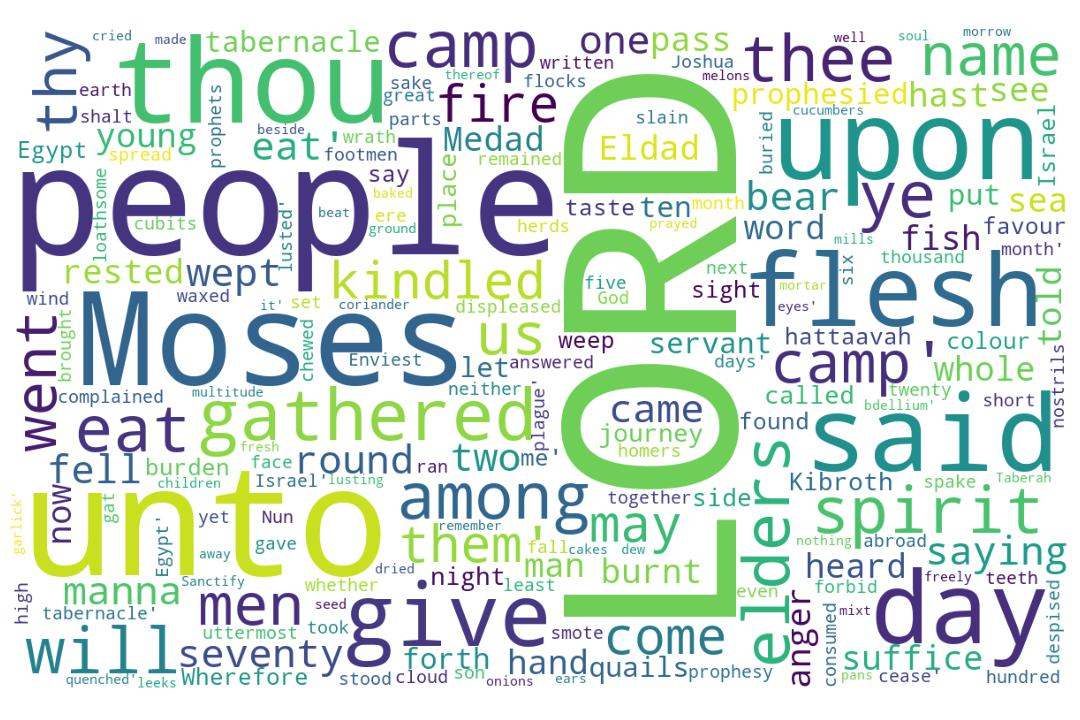
\includegraphics[width=\linewidth]{04OT-Numbers/Numbers11-WordCloud.jpg}
  \caption{Numbers 11 Word Cloud}
  \label{fig:Numbers 11 word Cloud}
\end{figure}


\marginpar{\scriptsize \centering \fcolorbox{bone}{lime}{\textbf{TROUBLE IN THE RANKS}}\\ (Numbers 11:1-35) \begin{compactenum}[I.][8]
    \item \textbf{Complaints about God's Provision} \index[scripture]{Numbers!Num 11:01}(Numbers 11:1)
    \item \textbf{Consumed on the Edges} \index[scripture]{Numbers!Num 11:01}(Numbers 11:1)
    \item \textbf{Closeness Matters} \index[scripture]{Numbers!Num 11:01}(Numbers 11:1)
    \item The \textbf{Cursed Extras} \index[scripture]{Numbers!Num 11:04}(Numbers 11:4)
    \item \textbf{Cucumbers Remembered} \index[scripture]{Numbers!Num 11:05}(Numbers 11:5)
    \item A \textbf{Council of Elders} \index[scripture]{Numbers!Num 11:16}(Numbers 11:16)
    \item The \textbf{Could of Empowerment} \index[scripture]{Numbers!Num 11:25}(Numbers 11:25)
    \item A \textbf{Clear Vision} \index[scripture]{Numbers!Num 11:29}(Numbers 11:29)
\end{compactenum}}



\footnote{\textcolor[cmyk]{0.99998,1,0,0}{\hyperlink{TOC}{Return to end of Table of Contents.}}}\footnote{\href{https://audiobible.com/bible/numbers_11.html}{\textcolor[cmyk]{0.99998,1,0,0}{Numbers 11 Audio}}}\textcolor[cmyk]{0.99998,1,0,0}{And \emph{when} the people \fcolorbox{bone}{lime}{complained}, it displeased the LORD: and the LORD heard \emph{it}; and his anger was kindled; and the fire of the LORD burnt among them, and \fcolorbox{bone}{lime}{consumed} \emph{them} \emph{that} \emph{were} in the \fcolorbox{bone}{lime}{uttermost} parts of the camp.}
[2] \textcolor[cmyk]{0.99998,1,0,0}{And the people cried unto Moses; and when Moses prayed unto the LORD, the fire was quenched.}
[3] \textcolor[cmyk]{0.99998,1,0,0}{And he called the name of the place Taberah: because the fire of the LORD burnt among them.}\\
\\
\P \textcolor[cmyk]{0.99998,1,0,0}{And the \fcolorbox{bone}{lime}{mixt multitude} that \emph{was} among them fell a lusting: and the children of Israel also wept again, and said, Who shall give us flesh to eat?}
[5] \textcolor[cmyk]{0.99998,1,0,0}{We remember the fish, which we did eat in Egypt freely; the \fcolorbox{bone}{lime}{cucumbers}, and the melons, and the leeks, and the onions, and the garlick:}
[6] \textcolor[cmyk]{0.99998,1,0,0}{But now our soul \emph{is} dried away: \emph{there} \emph{is} nothing at all, beside this manna, \emph{before} our eyes.}
[7] \textcolor[cmyk]{0.99998,1,0,0}{And the manna \emph{was} as coriander seed, and the colour thereof as the colour of bdellium.}
[8] \textcolor[cmyk]{0.99998,1,0,0}{\emph{And} the people went about, and gathered \emph{it}, and ground \emph{it} in mills, or beat \emph{it} in a mortar, and baked \emph{it} in pans, and made cakes of it: and the taste of it was as the taste of fresh oil.}
[9] \textcolor[cmyk]{0.99998,1,0,0}{And when the dew fell upon the camp in the night, the manna fell upon it.}
[10] \textcolor[cmyk]{0.99998,1,0,0}{Then Moses heard the people weep throughout their families, every man in the door of his tent: and the anger of the LORD was kindled greatly; Moses also was displeased.}
[11] \textcolor[cmyk]{0.99998,1,0,0}{And Moses said unto the LORD, Wherefore hast thou afflicted thy servant? and wherefore have I not found favour in thy sight, that thou layest the burden of all this people upon me?}
[12] \textcolor[cmyk]{0.99998,1,0,0}{Have I conceived all this people? have I begotten them, that thou shouldest say unto me, Carry them in thy bosom, as a nursing father beareth the sucking child, unto the land which thou swarest unto their fathers?}
[13] \textcolor[cmyk]{0.99998,1,0,0}{Whence should I have flesh to give unto all this people? for they weep unto me, saying, Give us flesh, that we may eat.}
[14] \textcolor[cmyk]{0.99998,1,0,0}{I am not able to bear all this people alone, because \emph{it} \emph{is} too heavy for me.}
[15] \textcolor[cmyk]{0.99998,1,0,0}{And if thou deal thus with me, kill me, I pray thee, out of hand, if I have found favour in thy sight; and let me not see my wretchedness.}\\
\\
\P \textcolor[cmyk]{0.99998,1,0,0}{And the LORD said unto Moses, Gather unto me \fcolorbox{bone}{lime}{seventy men} of the elders of Israel, whom thou knowest to be the elders of the people, and officers over them; and bring them unto the tabernacle of the congregation, that they may stand there with thee.}
[17] \textcolor[cmyk]{0.99998,1,0,0}{And I will come down and talk with thee there: and I will take of the spirit which \emph{is} upon thee, and will put \emph{it} upon them; and they shall bear the burden of the people with thee, that thou bear \emph{it} not thyself alone.}
[18] \textcolor[cmyk]{0.99998,1,0,0}{And say thou unto the people, Sanctify yourselves against to morrow, and ye shall eat flesh: for ye have wept in the ears of the LORD, saying, Who shall give us flesh to eat? for \emph{it} \emph{was} well with us in Egypt: therefore the LORD will give you flesh, and ye shall eat.}
[19] \textcolor[cmyk]{0.99998,1,0,0}{Ye shall not eat one day, nor two days, nor five days, neither ten days, nor twenty days;}
[20] \textcolor[cmyk]{0.99998,1,0,0}{\emph{But} even a whole month, until it come out at your nostrils, and it be loathsome unto you: because that ye have despised the LORD which \emph{is} among you, and have wept before him, saying, Why came we forth out of Egypt?}
[21] \textcolor[cmyk]{0.99998,1,0,0}{And Moses said, The people, among whom I \emph{am}, \emph{are} six hundred thousand footmen; and thou hast said, I will give them flesh, that they may eat a whole month.}
[22] \textcolor[cmyk]{0.99998,1,0,0}{Shall the flocks and the herds be slain for them, to suffice them? or shall all the fish of the sea be gathered together for them, to suffice them?}
[23] \textcolor[cmyk]{0.99998,1,0,0}{And the LORD said unto Moses, Is the LORD'S hand waxed short? thou shalt see now whether my word shall come to pass unto thee or not.}\\
\\
\P \textcolor[cmyk]{0.99998,1,0,0}{And Moses went out, and told the people the words of the LORD, and gathered the seventy men of the elders of the people, and set them round about the tabernacle.}
[25] \textcolor[cmyk]{0.99998,1,0,0}{And the LORD came down in a cloud, and spake unto him, and took of the spirit that \emph{was} upon him, and gave \emph{it} unto the seventy elders: and it came to pass, \emph{that}, when the spirit rested upon them, they \fcolorbox{bone}{lime}{prophesied}, and did not cease.}
[26] \textcolor[cmyk]{0.99998,1,0,0}{But there remained two \emph{of} \emph{the} men in the camp, the name of the one \emph{was} Eldad, and the name of the other Medad: and the spirit rested upon them; and they \emph{were} of them that were written, but went not out unto the tabernacle: and they prophesied in the camp.}
[27] \textcolor[cmyk]{0.99998,1,0,0}{And there ran a young man, and told Moses, and said, Eldad and Medad do prophesy in the camp.}
[28] \textcolor[cmyk]{0.99998,1,0,0}{And Joshua the son of Nun, the servant of Moses, \emph{one} of his young men, answered and said, My lord Moses, forbid them.}
[29] \textcolor[cmyk]{0.99998,1,0,0}{And Moses said unto him, Enviest thou for my sake? \fcolorbox{bone}{lime}{would God} that all the LORD'S people were prophets, \emph{and} that the LORD would put his spirit upon them!}
[30] \textcolor[cmyk]{0.99998,1,0,0}{And Moses gat him into the camp, he and the elders of Israel.}\\
\\
\P \textcolor[cmyk]{0.99998,1,0,0}{And there went forth a wind from the LORD, and brought quails from the sea, and let \emph{them} fall by the camp, as it were a day's journey on this side, and as it were a day's journey on the other side, round about the camp, and as it were two cubits \emph{high} upon the face of the earth.}
[32] \textcolor[cmyk]{0.99998,1,0,0}{And the people stood up all that day, and all \emph{that} night, and all the next day, and they gathered the quails: he that gathered least gathered ten homers: and they spread \emph{them} all abroad for themselves round about the camp.}
[33] \textcolor[cmyk]{0.99998,1,0,0}{And while the flesh \emph{was} yet between their teeth, ere it was chewed, the wrath of the LORD was kindled against the people, and the LORD smote the people with a very great plague.}
[34] \textcolor[cmyk]{0.99998,1,0,0}{And he called the name of that place Kibroth-hattaavah: because there they buried the people that lusted.}
[35] \textcolor[cmyk]{0.99998,1,0,0}{\emph{And} the people journeyed from Kibroth-hattaavah unto Hazeroth; and abode at Hazeroth.}
\index[NWIV]{40!Numbers!Num 11:1}\index[AWIP]{And!Numbers!Num 11:1}\index[AWIP]{\emph{when}!Numbers!Num 11:1}\index[AWIP]{the!Numbers!Num 11:1}\index[AWIP]{the!Numbers!Num 11:1 (2)}\index[AWIP]{the!Numbers!Num 11:1 (3)}\index[AWIP]{the!Numbers!Num 11:1 (4)}\index[AWIP]{the!Numbers!Num 11:1 (5)}\index[AWIP]{the!Numbers!Num 11:1 (6)}\index[AWIP]{the!Numbers!Num 11:1 (7)}\index[AWIP]{people!Numbers!Num 11:1}\index[AWIP]{complained!Numbers!Num 11:1}\index[AWIP]{it!Numbers!Num 11:1}\index[AWIP]{displeased!Numbers!Num 11:1}\index[AWIP]{LORD!Numbers!Num 11:1}\index[AWIP]{LORD!Numbers!Num 11:1 (2)}\index[AWIP]{LORD!Numbers!Num 11:1 (3)}\index[AWIP]{and!Numbers!Num 11:1}\index[AWIP]{and!Numbers!Num 11:1 (2)}\index[AWIP]{and!Numbers!Num 11:1 (3)}\index[AWIP]{and!Numbers!Num 11:1 (4)}\index[AWIP]{heard!Numbers!Num 11:1}\index[AWIP]{\emph{it}!Numbers!Num 11:1}\index[AWIP]{his!Numbers!Num 11:1}\index[AWIP]{anger!Numbers!Num 11:1}\index[AWIP]{was!Numbers!Num 11:1}\index[AWIP]{kindled!Numbers!Num 11:1}\index[AWIP]{fire!Numbers!Num 11:1}\index[AWIP]{of!Numbers!Num 11:1}\index[AWIP]{of!Numbers!Num 11:1 (2)}\index[AWIP]{burnt!Numbers!Num 11:1}\index[AWIP]{among!Numbers!Num 11:1}\index[AWIP]{them!Numbers!Num 11:1}\index[AWIP]{consumed!Numbers!Num 11:1}\index[AWIP]{\emph{them}!Numbers!Num 11:1}\index[AWIP]{\emph{that}!Numbers!Num 11:1}\index[AWIP]{\emph{were}!Numbers!Num 11:1}\index[AWIP]{in!Numbers!Num 11:1}\index[AWIP]{uttermost!Numbers!Num 11:1}\index[AWIP]{parts!Numbers!Num 11:1}\index[AWIP]{camp!Numbers!Num 11:1}\index[AWIP]{\emph{when}!Numbers!Num 11:1}\index[AWIP]{\emph{it}!Numbers!Num 11:1}\index[AWIP]{\emph{them}!Numbers!Num 11:1}\index[AWIP]{\emph{that}!Numbers!Num 11:1}\index[AWIP]{\emph{were}!Numbers!Num 11:1}

\index[NWIV]{17!Numbers!Num 11:2}\index[AWIP]{And!Numbers!Num 11:2}\index[AWIP]{the!Numbers!Num 11:2}\index[AWIP]{the!Numbers!Num 11:2 (2)}\index[AWIP]{the!Numbers!Num 11:2 (3)}\index[AWIP]{people!Numbers!Num 11:2}\index[AWIP]{cried!Numbers!Num 11:2}\index[AWIP]{unto!Numbers!Num 11:2}\index[AWIP]{unto!Numbers!Num 11:2 (2)}\index[AWIP]{Moses!Numbers!Num 11:2}\index[AWIP]{Moses!Numbers!Num 11:2 (2)}\index[AWIP]{and!Numbers!Num 11:2}\index[AWIP]{when!Numbers!Num 11:2}\index[AWIP]{prayed!Numbers!Num 11:2}\index[AWIP]{LORD!Numbers!Num 11:2}\index[AWIP]{fire!Numbers!Num 11:2}\index[AWIP]{was!Numbers!Num 11:2}\index[AWIP]{quenched!Numbers!Num 11:2}

\index[NWIV]{18!Numbers!Num 11:3}\index[AWIP]{And!Numbers!Num 11:3}\index[AWIP]{he!Numbers!Num 11:3}\index[AWIP]{called!Numbers!Num 11:3}\index[AWIP]{the!Numbers!Num 11:3}\index[AWIP]{the!Numbers!Num 11:3 (2)}\index[AWIP]{the!Numbers!Num 11:3 (3)}\index[AWIP]{the!Numbers!Num 11:3 (4)}\index[AWIP]{name!Numbers!Num 11:3}\index[AWIP]{of!Numbers!Num 11:3}\index[AWIP]{of!Numbers!Num 11:3 (2)}\index[AWIP]{place!Numbers!Num 11:3}\index[AWIP]{Taberah!Numbers!Num 11:3}\index[AWIP]{because!Numbers!Num 11:3}\index[AWIP]{fire!Numbers!Num 11:3}\index[AWIP]{LORD!Numbers!Num 11:3}\index[AWIP]{burnt!Numbers!Num 11:3}\index[AWIP]{among!Numbers!Num 11:3}\index[AWIP]{them!Numbers!Num 11:3}

\index[NWIV]{28!Numbers!Num 11:4}\index[AWIP]{And!Numbers!Num 11:4}\index[AWIP]{the!Numbers!Num 11:4}\index[AWIP]{the!Numbers!Num 11:4 (2)}\index[AWIP]{mixt!Numbers!Num 11:4}\index[AWIP]{multitude!Numbers!Num 11:4}\index[AWIP]{that!Numbers!Num 11:4}\index[AWIP]{\emph{was}!Numbers!Num 11:4}\index[AWIP]{among!Numbers!Num 11:4}\index[AWIP]{them!Numbers!Num 11:4}\index[AWIP]{fell!Numbers!Num 11:4}\index[AWIP]{a!Numbers!Num 11:4}\index[AWIP]{lusting!Numbers!Num 11:4}\index[AWIP]{and!Numbers!Num 11:4}\index[AWIP]{and!Numbers!Num 11:4 (2)}\index[AWIP]{children!Numbers!Num 11:4}\index[AWIP]{of!Numbers!Num 11:4}\index[AWIP]{Israel!Numbers!Num 11:4}\index[AWIP]{also!Numbers!Num 11:4}\index[AWIP]{wept!Numbers!Num 11:4}\index[AWIP]{again!Numbers!Num 11:4}\index[AWIP]{said!Numbers!Num 11:4}\index[AWIP]{Who!Numbers!Num 11:4}\index[AWIP]{shall!Numbers!Num 11:4}\index[AWIP]{give!Numbers!Num 11:4}\index[AWIP]{us!Numbers!Num 11:4}\index[AWIP]{flesh!Numbers!Num 11:4}\index[AWIP]{to!Numbers!Num 11:4}\index[AWIP]{eat?!Numbers!Num 11:4}\index[AWIP]{\emph{was}!Numbers!Num 11:4}

\index[NWIV]{25!Numbers!Num 11:5}\index[AWIP]{We!Numbers!Num 11:5}\index[AWIP]{remember!Numbers!Num 11:5}\index[AWIP]{the!Numbers!Num 11:5}\index[AWIP]{the!Numbers!Num 11:5 (2)}\index[AWIP]{the!Numbers!Num 11:5 (3)}\index[AWIP]{the!Numbers!Num 11:5 (4)}\index[AWIP]{the!Numbers!Num 11:5 (5)}\index[AWIP]{the!Numbers!Num 11:5 (6)}\index[AWIP]{fish!Numbers!Num 11:5}\index[AWIP]{which!Numbers!Num 11:5}\index[AWIP]{we!Numbers!Num 11:5}\index[AWIP]{did!Numbers!Num 11:5}\index[AWIP]{eat!Numbers!Num 11:5}\index[AWIP]{in!Numbers!Num 11:5}\index[AWIP]{Egypt!Numbers!Num 11:5}\index[AWIP]{freely!Numbers!Num 11:5}\index[AWIP]{cucumbers!Numbers!Num 11:5}\index[AWIP]{and!Numbers!Num 11:5}\index[AWIP]{and!Numbers!Num 11:5 (2)}\index[AWIP]{and!Numbers!Num 11:5 (3)}\index[AWIP]{and!Numbers!Num 11:5 (4)}\index[AWIP]{melons!Numbers!Num 11:5}\index[AWIP]{leeks!Numbers!Num 11:5}\index[AWIP]{onions!Numbers!Num 11:5}\index[AWIP]{garlick!Numbers!Num 11:5}

\index[NWIV]{18!Numbers!Num 11:6}\index[AWIP]{But!Numbers!Num 11:6}\index[AWIP]{now!Numbers!Num 11:6}\index[AWIP]{our!Numbers!Num 11:6}\index[AWIP]{our!Numbers!Num 11:6 (2)}\index[AWIP]{soul!Numbers!Num 11:6}\index[AWIP]{\emph{is}!Numbers!Num 11:6}\index[AWIP]{\emph{is}!Numbers!Num 11:6 (2)}\index[AWIP]{dried!Numbers!Num 11:6}\index[AWIP]{away!Numbers!Num 11:6}\index[AWIP]{\emph{there}!Numbers!Num 11:6}\index[AWIP]{nothing!Numbers!Num 11:6}\index[AWIP]{at!Numbers!Num 11:6}\index[AWIP]{all!Numbers!Num 11:6}\index[AWIP]{beside!Numbers!Num 11:6}\index[AWIP]{this!Numbers!Num 11:6}\index[AWIP]{manna!Numbers!Num 11:6}\index[AWIP]{\emph{before}!Numbers!Num 11:6}\index[AWIP]{eyes!Numbers!Num 11:6}\index[AWIP]{\emph{is}!Numbers!Num 11:6}\index[AWIP]{\emph{is}!Numbers!Num 11:6 (2)}\index[AWIP]{\emph{there}!Numbers!Num 11:6}\index[AWIP]{\emph{before}!Numbers!Num 11:6}

\index[NWIV]{16!Numbers!Num 11:7}\index[AWIP]{And!Numbers!Num 11:7}\index[AWIP]{the!Numbers!Num 11:7}\index[AWIP]{the!Numbers!Num 11:7 (2)}\index[AWIP]{the!Numbers!Num 11:7 (3)}\index[AWIP]{manna!Numbers!Num 11:7}\index[AWIP]{\emph{was}!Numbers!Num 11:7}\index[AWIP]{as!Numbers!Num 11:7}\index[AWIP]{as!Numbers!Num 11:7 (2)}\index[AWIP]{coriander!Numbers!Num 11:7}\index[AWIP]{seed!Numbers!Num 11:7}\index[AWIP]{and!Numbers!Num 11:7}\index[AWIP]{colour!Numbers!Num 11:7}\index[AWIP]{colour!Numbers!Num 11:7 (2)}\index[AWIP]{thereof!Numbers!Num 11:7}\index[AWIP]{of!Numbers!Num 11:7}\index[AWIP]{bdellium!Numbers!Num 11:7}\index[AWIP]{\emph{was}!Numbers!Num 11:7}

\index[NWIV]{41!Numbers!Num 11:8}\index[AWIP]{\emph{And}!Numbers!Num 11:8}\index[AWIP]{the!Numbers!Num 11:8}\index[AWIP]{the!Numbers!Num 11:8 (2)}\index[AWIP]{the!Numbers!Num 11:8 (3)}\index[AWIP]{people!Numbers!Num 11:8}\index[AWIP]{went!Numbers!Num 11:8}\index[AWIP]{about!Numbers!Num 11:8}\index[AWIP]{and!Numbers!Num 11:8}\index[AWIP]{and!Numbers!Num 11:8 (2)}\index[AWIP]{and!Numbers!Num 11:8 (3)}\index[AWIP]{and!Numbers!Num 11:8 (4)}\index[AWIP]{and!Numbers!Num 11:8 (5)}\index[AWIP]{gathered!Numbers!Num 11:8}\index[AWIP]{\emph{it}!Numbers!Num 11:8}\index[AWIP]{\emph{it}!Numbers!Num 11:8 (2)}\index[AWIP]{\emph{it}!Numbers!Num 11:8 (3)}\index[AWIP]{\emph{it}!Numbers!Num 11:8 (4)}\index[AWIP]{ground!Numbers!Num 11:8}\index[AWIP]{in!Numbers!Num 11:8}\index[AWIP]{in!Numbers!Num 11:8 (2)}\index[AWIP]{in!Numbers!Num 11:8 (3)}\index[AWIP]{mills!Numbers!Num 11:8}\index[AWIP]{or!Numbers!Num 11:8}\index[AWIP]{beat!Numbers!Num 11:8}\index[AWIP]{a!Numbers!Num 11:8}\index[AWIP]{mortar!Numbers!Num 11:8}\index[AWIP]{baked!Numbers!Num 11:8}\index[AWIP]{pans!Numbers!Num 11:8}\index[AWIP]{made!Numbers!Num 11:8}\index[AWIP]{cakes!Numbers!Num 11:8}\index[AWIP]{of!Numbers!Num 11:8}\index[AWIP]{of!Numbers!Num 11:8 (2)}\index[AWIP]{of!Numbers!Num 11:8 (3)}\index[AWIP]{it!Numbers!Num 11:8}\index[AWIP]{it!Numbers!Num 11:8 (2)}\index[AWIP]{taste!Numbers!Num 11:8}\index[AWIP]{taste!Numbers!Num 11:8 (2)}\index[AWIP]{was!Numbers!Num 11:8}\index[AWIP]{as!Numbers!Num 11:8}\index[AWIP]{fresh!Numbers!Num 11:8}\index[AWIP]{oil!Numbers!Num 11:8}\index[AWIP]{\emph{And}!Numbers!Num 11:8}\index[AWIP]{\emph{it}!Numbers!Num 11:8}\index[AWIP]{\emph{it}!Numbers!Num 11:8 (2)}\index[AWIP]{\emph{it}!Numbers!Num 11:8 (3)}\index[AWIP]{\emph{it}!Numbers!Num 11:8 (4)}

\index[NWIV]{16!Numbers!Num 11:9}\index[AWIP]{And!Numbers!Num 11:9}\index[AWIP]{when!Numbers!Num 11:9}\index[AWIP]{the!Numbers!Num 11:9}\index[AWIP]{the!Numbers!Num 11:9 (2)}\index[AWIP]{the!Numbers!Num 11:9 (3)}\index[AWIP]{the!Numbers!Num 11:9 (4)}\index[AWIP]{dew!Numbers!Num 11:9}\index[AWIP]{fell!Numbers!Num 11:9}\index[AWIP]{fell!Numbers!Num 11:9 (2)}\index[AWIP]{upon!Numbers!Num 11:9}\index[AWIP]{upon!Numbers!Num 11:9 (2)}\index[AWIP]{camp!Numbers!Num 11:9}\index[AWIP]{in!Numbers!Num 11:9}\index[AWIP]{night!Numbers!Num 11:9}\index[AWIP]{manna!Numbers!Num 11:9}\index[AWIP]{it!Numbers!Num 11:9}

\index[NWIV]{30!Numbers!Num 11:10}\index[AWIP]{Then!Numbers!Num 11:10}\index[AWIP]{Moses!Numbers!Num 11:10}\index[AWIP]{Moses!Numbers!Num 11:10 (2)}\index[AWIP]{heard!Numbers!Num 11:10}\index[AWIP]{the!Numbers!Num 11:10}\index[AWIP]{the!Numbers!Num 11:10 (2)}\index[AWIP]{the!Numbers!Num 11:10 (3)}\index[AWIP]{the!Numbers!Num 11:10 (4)}\index[AWIP]{people!Numbers!Num 11:10}\index[AWIP]{weep!Numbers!Num 11:10}\index[AWIP]{throughout!Numbers!Num 11:10}\index[AWIP]{their!Numbers!Num 11:10}\index[AWIP]{families!Numbers!Num 11:10}\index[AWIP]{every!Numbers!Num 11:10}\index[AWIP]{man!Numbers!Num 11:10}\index[AWIP]{in!Numbers!Num 11:10}\index[AWIP]{door!Numbers!Num 11:10}\index[AWIP]{of!Numbers!Num 11:10}\index[AWIP]{of!Numbers!Num 11:10 (2)}\index[AWIP]{his!Numbers!Num 11:10}\index[AWIP]{tent!Numbers!Num 11:10}\index[AWIP]{and!Numbers!Num 11:10}\index[AWIP]{anger!Numbers!Num 11:10}\index[AWIP]{LORD!Numbers!Num 11:10}\index[AWIP]{was!Numbers!Num 11:10}\index[AWIP]{was!Numbers!Num 11:10 (2)}\index[AWIP]{kindled!Numbers!Num 11:10}\index[AWIP]{greatly!Numbers!Num 11:10}\index[AWIP]{also!Numbers!Num 11:10}\index[AWIP]{displeased!Numbers!Num 11:10}

\index[NWIV]{33!Numbers!Num 11:11}\index[AWIP]{And!Numbers!Num 11:11}\index[AWIP]{Moses!Numbers!Num 11:11}\index[AWIP]{said!Numbers!Num 11:11}\index[AWIP]{unto!Numbers!Num 11:11}\index[AWIP]{the!Numbers!Num 11:11}\index[AWIP]{the!Numbers!Num 11:11 (2)}\index[AWIP]{LORD!Numbers!Num 11:11}\index[AWIP]{Wherefore!Numbers!Num 11:11}\index[AWIP]{hast!Numbers!Num 11:11}\index[AWIP]{thou!Numbers!Num 11:11}\index[AWIP]{thou!Numbers!Num 11:11 (2)}\index[AWIP]{afflicted!Numbers!Num 11:11}\index[AWIP]{thy!Numbers!Num 11:11}\index[AWIP]{thy!Numbers!Num 11:11 (2)}\index[AWIP]{servant?!Numbers!Num 11:11}\index[AWIP]{and!Numbers!Num 11:11}\index[AWIP]{wherefore!Numbers!Num 11:11}\index[AWIP]{have!Numbers!Num 11:11}\index[AWIP]{I!Numbers!Num 11:11}\index[AWIP]{not!Numbers!Num 11:11}\index[AWIP]{found!Numbers!Num 11:11}\index[AWIP]{favour!Numbers!Num 11:11}\index[AWIP]{in!Numbers!Num 11:11}\index[AWIP]{sight!Numbers!Num 11:11}\index[AWIP]{that!Numbers!Num 11:11}\index[AWIP]{layest!Numbers!Num 11:11}\index[AWIP]{burden!Numbers!Num 11:11}\index[AWIP]{of!Numbers!Num 11:11}\index[AWIP]{all!Numbers!Num 11:11}\index[AWIP]{this!Numbers!Num 11:11}\index[AWIP]{people!Numbers!Num 11:11}\index[AWIP]{upon!Numbers!Num 11:11}\index[AWIP]{me?!Numbers!Num 11:11}

\index[NWIV]{38!Numbers!Num 11:12}\index[AWIP]{Have!Numbers!Num 11:12}\index[AWIP]{I!Numbers!Num 11:12}\index[AWIP]{I!Numbers!Num 11:12 (2)}\index[AWIP]{conceived!Numbers!Num 11:12}\index[AWIP]{all!Numbers!Num 11:12}\index[AWIP]{this!Numbers!Num 11:12}\index[AWIP]{people?!Numbers!Num 11:12}\index[AWIP]{have!Numbers!Num 11:12}\index[AWIP]{begotten!Numbers!Num 11:12}\index[AWIP]{them!Numbers!Num 11:12}\index[AWIP]{them!Numbers!Num 11:12 (2)}\index[AWIP]{that!Numbers!Num 11:12}\index[AWIP]{thou!Numbers!Num 11:12}\index[AWIP]{thou!Numbers!Num 11:12 (2)}\index[AWIP]{shouldest!Numbers!Num 11:12}\index[AWIP]{say!Numbers!Num 11:12}\index[AWIP]{unto!Numbers!Num 11:12}\index[AWIP]{unto!Numbers!Num 11:12 (2)}\index[AWIP]{unto!Numbers!Num 11:12 (3)}\index[AWIP]{me!Numbers!Num 11:12}\index[AWIP]{Carry!Numbers!Num 11:12}\index[AWIP]{in!Numbers!Num 11:12}\index[AWIP]{thy!Numbers!Num 11:12}\index[AWIP]{bosom!Numbers!Num 11:12}\index[AWIP]{as!Numbers!Num 11:12}\index[AWIP]{a!Numbers!Num 11:12}\index[AWIP]{nursing!Numbers!Num 11:12}\index[AWIP]{father!Numbers!Num 11:12}\index[AWIP]{beareth!Numbers!Num 11:12}\index[AWIP]{the!Numbers!Num 11:12}\index[AWIP]{the!Numbers!Num 11:12 (2)}\index[AWIP]{sucking!Numbers!Num 11:12}\index[AWIP]{child!Numbers!Num 11:12}\index[AWIP]{land!Numbers!Num 11:12}\index[AWIP]{which!Numbers!Num 11:12}\index[AWIP]{swarest!Numbers!Num 11:12}\index[AWIP]{their!Numbers!Num 11:12}\index[AWIP]{fathers?!Numbers!Num 11:12}

\index[NWIV]{24!Numbers!Num 11:13}\index[AWIP]{Whence!Numbers!Num 11:13}\index[AWIP]{should!Numbers!Num 11:13}\index[AWIP]{I!Numbers!Num 11:13}\index[AWIP]{have!Numbers!Num 11:13}\index[AWIP]{flesh!Numbers!Num 11:13}\index[AWIP]{flesh!Numbers!Num 11:13 (2)}\index[AWIP]{to!Numbers!Num 11:13}\index[AWIP]{give!Numbers!Num 11:13}\index[AWIP]{unto!Numbers!Num 11:13}\index[AWIP]{unto!Numbers!Num 11:13 (2)}\index[AWIP]{all!Numbers!Num 11:13}\index[AWIP]{this!Numbers!Num 11:13}\index[AWIP]{people?!Numbers!Num 11:13}\index[AWIP]{for!Numbers!Num 11:13}\index[AWIP]{they!Numbers!Num 11:13}\index[AWIP]{weep!Numbers!Num 11:13}\index[AWIP]{me!Numbers!Num 11:13}\index[AWIP]{saying!Numbers!Num 11:13}\index[AWIP]{Give!Numbers!Num 11:13}\index[AWIP]{us!Numbers!Num 11:13}\index[AWIP]{that!Numbers!Num 11:13}\index[AWIP]{we!Numbers!Num 11:13}\index[AWIP]{may!Numbers!Num 11:13}\index[AWIP]{eat!Numbers!Num 11:13}

\index[NWIV]{17!Numbers!Num 11:14}\index[AWIP]{I!Numbers!Num 11:14}\index[AWIP]{am!Numbers!Num 11:14}\index[AWIP]{not!Numbers!Num 11:14}\index[AWIP]{able!Numbers!Num 11:14}\index[AWIP]{to!Numbers!Num 11:14}\index[AWIP]{bear!Numbers!Num 11:14}\index[AWIP]{all!Numbers!Num 11:14}\index[AWIP]{this!Numbers!Num 11:14}\index[AWIP]{people!Numbers!Num 11:14}\index[AWIP]{alone!Numbers!Num 11:14}\index[AWIP]{because!Numbers!Num 11:14}\index[AWIP]{\emph{it}!Numbers!Num 11:14}\index[AWIP]{\emph{is}!Numbers!Num 11:14}\index[AWIP]{too!Numbers!Num 11:14}\index[AWIP]{heavy!Numbers!Num 11:14}\index[AWIP]{for!Numbers!Num 11:14}\index[AWIP]{me!Numbers!Num 11:14}\index[AWIP]{\emph{it}!Numbers!Num 11:14}\index[AWIP]{\emph{is}!Numbers!Num 11:14}

\index[NWIV]{30!Numbers!Num 11:15}\index[AWIP]{And!Numbers!Num 11:15}\index[AWIP]{if!Numbers!Num 11:15}\index[AWIP]{if!Numbers!Num 11:15 (2)}\index[AWIP]{thou!Numbers!Num 11:15}\index[AWIP]{deal!Numbers!Num 11:15}\index[AWIP]{thus!Numbers!Num 11:15}\index[AWIP]{with!Numbers!Num 11:15}\index[AWIP]{me!Numbers!Num 11:15}\index[AWIP]{me!Numbers!Num 11:15 (2)}\index[AWIP]{me!Numbers!Num 11:15 (3)}\index[AWIP]{kill!Numbers!Num 11:15}\index[AWIP]{I!Numbers!Num 11:15}\index[AWIP]{I!Numbers!Num 11:15 (2)}\index[AWIP]{pray!Numbers!Num 11:15}\index[AWIP]{thee!Numbers!Num 11:15}\index[AWIP]{out!Numbers!Num 11:15}\index[AWIP]{of!Numbers!Num 11:15}\index[AWIP]{hand!Numbers!Num 11:15}\index[AWIP]{have!Numbers!Num 11:15}\index[AWIP]{found!Numbers!Num 11:15}\index[AWIP]{favour!Numbers!Num 11:15}\index[AWIP]{in!Numbers!Num 11:15}\index[AWIP]{thy!Numbers!Num 11:15}\index[AWIP]{sight!Numbers!Num 11:15}\index[AWIP]{and!Numbers!Num 11:15}\index[AWIP]{let!Numbers!Num 11:15}\index[AWIP]{not!Numbers!Num 11:15}\index[AWIP]{see!Numbers!Num 11:15}\index[AWIP]{my!Numbers!Num 11:15}\index[AWIP]{wretchedness!Numbers!Num 11:15}

\index[NWIV]{46!Numbers!Num 11:16}\index[AWIP]{And!Numbers!Num 11:16}\index[AWIP]{the!Numbers!Num 11:16}\index[AWIP]{the!Numbers!Num 11:16 (2)}\index[AWIP]{the!Numbers!Num 11:16 (3)}\index[AWIP]{the!Numbers!Num 11:16 (4)}\index[AWIP]{the!Numbers!Num 11:16 (5)}\index[AWIP]{the!Numbers!Num 11:16 (6)}\index[AWIP]{LORD!Numbers!Num 11:16}\index[AWIP]{said!Numbers!Num 11:16}\index[AWIP]{unto!Numbers!Num 11:16}\index[AWIP]{unto!Numbers!Num 11:16 (2)}\index[AWIP]{unto!Numbers!Num 11:16 (3)}\index[AWIP]{Moses!Numbers!Num 11:16}\index[AWIP]{Gather!Numbers!Num 11:16}\index[AWIP]{me!Numbers!Num 11:16}\index[AWIP]{seventy!Numbers!Num 11:16}\index[AWIP]{men!Numbers!Num 11:16}\index[AWIP]{of!Numbers!Num 11:16}\index[AWIP]{of!Numbers!Num 11:16 (2)}\index[AWIP]{of!Numbers!Num 11:16 (3)}\index[AWIP]{of!Numbers!Num 11:16 (4)}\index[AWIP]{elders!Numbers!Num 11:16}\index[AWIP]{elders!Numbers!Num 11:16 (2)}\index[AWIP]{Israel!Numbers!Num 11:16}\index[AWIP]{whom!Numbers!Num 11:16}\index[AWIP]{thou!Numbers!Num 11:16}\index[AWIP]{knowest!Numbers!Num 11:16}\index[AWIP]{to!Numbers!Num 11:16}\index[AWIP]{be!Numbers!Num 11:16}\index[AWIP]{people!Numbers!Num 11:16}\index[AWIP]{and!Numbers!Num 11:16}\index[AWIP]{and!Numbers!Num 11:16 (2)}\index[AWIP]{officers!Numbers!Num 11:16}\index[AWIP]{over!Numbers!Num 11:16}\index[AWIP]{them!Numbers!Num 11:16}\index[AWIP]{them!Numbers!Num 11:16 (2)}\index[AWIP]{bring!Numbers!Num 11:16}\index[AWIP]{tabernacle!Numbers!Num 11:16}\index[AWIP]{congregation!Numbers!Num 11:16}\index[AWIP]{that!Numbers!Num 11:16}\index[AWIP]{they!Numbers!Num 11:16}\index[AWIP]{may!Numbers!Num 11:16}\index[AWIP]{stand!Numbers!Num 11:16}\index[AWIP]{there!Numbers!Num 11:16}\index[AWIP]{with!Numbers!Num 11:16}\index[AWIP]{thee!Numbers!Num 11:16}

\index[NWIV]{45!Numbers!Num 11:17}\index[AWIP]{And!Numbers!Num 11:17}\index[AWIP]{I!Numbers!Num 11:17}\index[AWIP]{I!Numbers!Num 11:17 (2)}\index[AWIP]{will!Numbers!Num 11:17}\index[AWIP]{will!Numbers!Num 11:17 (2)}\index[AWIP]{will!Numbers!Num 11:17 (3)}\index[AWIP]{come!Numbers!Num 11:17}\index[AWIP]{down!Numbers!Num 11:17}\index[AWIP]{and!Numbers!Num 11:17}\index[AWIP]{and!Numbers!Num 11:17 (2)}\index[AWIP]{and!Numbers!Num 11:17 (3)}\index[AWIP]{and!Numbers!Num 11:17 (4)}\index[AWIP]{talk!Numbers!Num 11:17}\index[AWIP]{with!Numbers!Num 11:17}\index[AWIP]{with!Numbers!Num 11:17 (2)}\index[AWIP]{thee!Numbers!Num 11:17}\index[AWIP]{thee!Numbers!Num 11:17 (2)}\index[AWIP]{thee!Numbers!Num 11:17 (3)}\index[AWIP]{there!Numbers!Num 11:17}\index[AWIP]{take!Numbers!Num 11:17}\index[AWIP]{of!Numbers!Num 11:17}\index[AWIP]{of!Numbers!Num 11:17 (2)}\index[AWIP]{the!Numbers!Num 11:17}\index[AWIP]{the!Numbers!Num 11:17 (2)}\index[AWIP]{the!Numbers!Num 11:17 (3)}\index[AWIP]{spirit!Numbers!Num 11:17}\index[AWIP]{which!Numbers!Num 11:17}\index[AWIP]{\emph{is}!Numbers!Num 11:17}\index[AWIP]{upon!Numbers!Num 11:17}\index[AWIP]{upon!Numbers!Num 11:17 (2)}\index[AWIP]{put!Numbers!Num 11:17}\index[AWIP]{\emph{it}!Numbers!Num 11:17}\index[AWIP]{\emph{it}!Numbers!Num 11:17 (2)}\index[AWIP]{them!Numbers!Num 11:17}\index[AWIP]{they!Numbers!Num 11:17}\index[AWIP]{shall!Numbers!Num 11:17}\index[AWIP]{bear!Numbers!Num 11:17}\index[AWIP]{bear!Numbers!Num 11:17 (2)}\index[AWIP]{burden!Numbers!Num 11:17}\index[AWIP]{people!Numbers!Num 11:17}\index[AWIP]{that!Numbers!Num 11:17}\index[AWIP]{thou!Numbers!Num 11:17}\index[AWIP]{not!Numbers!Num 11:17}\index[AWIP]{thyself!Numbers!Num 11:17}\index[AWIP]{alone!Numbers!Num 11:17}\index[AWIP]{\emph{is}!Numbers!Num 11:17}\index[AWIP]{\emph{it}!Numbers!Num 11:17}\index[AWIP]{\emph{it}!Numbers!Num 11:17 (2)}

\index[NWIV]{53!Numbers!Num 11:18}\index[AWIP]{And!Numbers!Num 11:18}\index[AWIP]{say!Numbers!Num 11:18}\index[AWIP]{thou!Numbers!Num 11:18}\index[AWIP]{unto!Numbers!Num 11:18}\index[AWIP]{the!Numbers!Num 11:18}\index[AWIP]{the!Numbers!Num 11:18 (2)}\index[AWIP]{the!Numbers!Num 11:18 (3)}\index[AWIP]{the!Numbers!Num 11:18 (4)}\index[AWIP]{people!Numbers!Num 11:18}\index[AWIP]{Sanctify!Numbers!Num 11:18}\index[AWIP]{yourselves!Numbers!Num 11:18}\index[AWIP]{against!Numbers!Num 11:18}\index[AWIP]{to!Numbers!Num 11:18}\index[AWIP]{to!Numbers!Num 11:18 (2)}\index[AWIP]{morrow!Numbers!Num 11:18}\index[AWIP]{and!Numbers!Num 11:18}\index[AWIP]{and!Numbers!Num 11:18 (2)}\index[AWIP]{ye!Numbers!Num 11:18}\index[AWIP]{ye!Numbers!Num 11:18 (2)}\index[AWIP]{ye!Numbers!Num 11:18 (3)}\index[AWIP]{shall!Numbers!Num 11:18}\index[AWIP]{shall!Numbers!Num 11:18 (2)}\index[AWIP]{shall!Numbers!Num 11:18 (3)}\index[AWIP]{eat!Numbers!Num 11:18}\index[AWIP]{eat!Numbers!Num 11:18 (2)}\index[AWIP]{flesh!Numbers!Num 11:18}\index[AWIP]{flesh!Numbers!Num 11:18 (2)}\index[AWIP]{flesh!Numbers!Num 11:18 (3)}\index[AWIP]{for!Numbers!Num 11:18}\index[AWIP]{for!Numbers!Num 11:18 (2)}\index[AWIP]{have!Numbers!Num 11:18}\index[AWIP]{wept!Numbers!Num 11:18}\index[AWIP]{in!Numbers!Num 11:18}\index[AWIP]{in!Numbers!Num 11:18 (2)}\index[AWIP]{ears!Numbers!Num 11:18}\index[AWIP]{of!Numbers!Num 11:18}\index[AWIP]{LORD!Numbers!Num 11:18}\index[AWIP]{LORD!Numbers!Num 11:18 (2)}\index[AWIP]{saying!Numbers!Num 11:18}\index[AWIP]{Who!Numbers!Num 11:18}\index[AWIP]{give!Numbers!Num 11:18}\index[AWIP]{give!Numbers!Num 11:18 (2)}\index[AWIP]{us!Numbers!Num 11:18}\index[AWIP]{us!Numbers!Num 11:18 (2)}\index[AWIP]{eat?!Numbers!Num 11:18}\index[AWIP]{\emph{it}!Numbers!Num 11:18}\index[AWIP]{\emph{was}!Numbers!Num 11:18}\index[AWIP]{well!Numbers!Num 11:18}\index[AWIP]{with!Numbers!Num 11:18}\index[AWIP]{Egypt!Numbers!Num 11:18}\index[AWIP]{therefore!Numbers!Num 11:18}\index[AWIP]{will!Numbers!Num 11:18}\index[AWIP]{you!Numbers!Num 11:18}\index[AWIP]{\emph{it}!Numbers!Num 11:18}\index[AWIP]{\emph{was}!Numbers!Num 11:18}

\index[NWIV]{18!Numbers!Num 11:19}\index[AWIP]{Ye!Numbers!Num 11:19}\index[AWIP]{shall!Numbers!Num 11:19}\index[AWIP]{not!Numbers!Num 11:19}\index[AWIP]{eat!Numbers!Num 11:19}\index[AWIP]{one!Numbers!Num 11:19}\index[AWIP]{day!Numbers!Num 11:19}\index[AWIP]{nor!Numbers!Num 11:19}\index[AWIP]{nor!Numbers!Num 11:19 (2)}\index[AWIP]{nor!Numbers!Num 11:19 (3)}\index[AWIP]{two!Numbers!Num 11:19}\index[AWIP]{days!Numbers!Num 11:19}\index[AWIP]{days!Numbers!Num 11:19 (2)}\index[AWIP]{days!Numbers!Num 11:19 (3)}\index[AWIP]{days!Numbers!Num 11:19 (4)}\index[AWIP]{five!Numbers!Num 11:19}\index[AWIP]{neither!Numbers!Num 11:19}\index[AWIP]{ten!Numbers!Num 11:19}\index[AWIP]{twenty!Numbers!Num 11:19}

\index[NWIV]{42!Numbers!Num 11:20}\index[AWIP]{\emph{But}!Numbers!Num 11:20}\index[AWIP]{even!Numbers!Num 11:20}\index[AWIP]{a!Numbers!Num 11:20}\index[AWIP]{whole!Numbers!Num 11:20}\index[AWIP]{month!Numbers!Num 11:20}\index[AWIP]{until!Numbers!Num 11:20}\index[AWIP]{it!Numbers!Num 11:20}\index[AWIP]{it!Numbers!Num 11:20 (2)}\index[AWIP]{come!Numbers!Num 11:20}\index[AWIP]{out!Numbers!Num 11:20}\index[AWIP]{out!Numbers!Num 11:20 (2)}\index[AWIP]{at!Numbers!Num 11:20}\index[AWIP]{your!Numbers!Num 11:20}\index[AWIP]{nostrils!Numbers!Num 11:20}\index[AWIP]{and!Numbers!Num 11:20}\index[AWIP]{and!Numbers!Num 11:20 (2)}\index[AWIP]{be!Numbers!Num 11:20}\index[AWIP]{loathsome!Numbers!Num 11:20}\index[AWIP]{unto!Numbers!Num 11:20}\index[AWIP]{you!Numbers!Num 11:20}\index[AWIP]{you!Numbers!Num 11:20 (2)}\index[AWIP]{because!Numbers!Num 11:20}\index[AWIP]{that!Numbers!Num 11:20}\index[AWIP]{ye!Numbers!Num 11:20}\index[AWIP]{have!Numbers!Num 11:20}\index[AWIP]{have!Numbers!Num 11:20 (2)}\index[AWIP]{despised!Numbers!Num 11:20}\index[AWIP]{the!Numbers!Num 11:20}\index[AWIP]{LORD!Numbers!Num 11:20}\index[AWIP]{which!Numbers!Num 11:20}\index[AWIP]{\emph{is}!Numbers!Num 11:20}\index[AWIP]{among!Numbers!Num 11:20}\index[AWIP]{wept!Numbers!Num 11:20}\index[AWIP]{before!Numbers!Num 11:20}\index[AWIP]{him!Numbers!Num 11:20}\index[AWIP]{saying!Numbers!Num 11:20}\index[AWIP]{Why!Numbers!Num 11:20}\index[AWIP]{came!Numbers!Num 11:20}\index[AWIP]{we!Numbers!Num 11:20}\index[AWIP]{forth!Numbers!Num 11:20}\index[AWIP]{of!Numbers!Num 11:20}\index[AWIP]{Egypt?!Numbers!Num 11:20}\index[AWIP]{\emph{But}!Numbers!Num 11:20}\index[AWIP]{\emph{is}!Numbers!Num 11:20}

\index[NWIV]{30!Numbers!Num 11:21}\index[AWIP]{And!Numbers!Num 11:21}\index[AWIP]{Moses!Numbers!Num 11:21}\index[AWIP]{said!Numbers!Num 11:21}\index[AWIP]{said!Numbers!Num 11:21 (2)}\index[AWIP]{The!Numbers!Num 11:21}\index[AWIP]{people!Numbers!Num 11:21}\index[AWIP]{among!Numbers!Num 11:21}\index[AWIP]{whom!Numbers!Num 11:21}\index[AWIP]{I!Numbers!Num 11:21}\index[AWIP]{I!Numbers!Num 11:21 (2)}\index[AWIP]{\emph{am}!Numbers!Num 11:21}\index[AWIP]{\emph{are}!Numbers!Num 11:21}\index[AWIP]{six!Numbers!Num 11:21}\index[AWIP]{hundred!Numbers!Num 11:21}\index[AWIP]{thousand!Numbers!Num 11:21}\index[AWIP]{footmen!Numbers!Num 11:21}\index[AWIP]{and!Numbers!Num 11:21}\index[AWIP]{thou!Numbers!Num 11:21}\index[AWIP]{hast!Numbers!Num 11:21}\index[AWIP]{will!Numbers!Num 11:21}\index[AWIP]{give!Numbers!Num 11:21}\index[AWIP]{them!Numbers!Num 11:21}\index[AWIP]{flesh!Numbers!Num 11:21}\index[AWIP]{that!Numbers!Num 11:21}\index[AWIP]{they!Numbers!Num 11:21}\index[AWIP]{may!Numbers!Num 11:21}\index[AWIP]{eat!Numbers!Num 11:21}\index[AWIP]{a!Numbers!Num 11:21}\index[AWIP]{whole!Numbers!Num 11:21}\index[AWIP]{month!Numbers!Num 11:21}\index[AWIP]{\emph{am}!Numbers!Num 11:21}\index[AWIP]{\emph{are}!Numbers!Num 11:21}

\index[NWIV]{29!Numbers!Num 11:22}\index[AWIP]{Shall!Numbers!Num 11:22}\index[AWIP]{the!Numbers!Num 11:22}\index[AWIP]{the!Numbers!Num 11:22 (2)}\index[AWIP]{the!Numbers!Num 11:22 (3)}\index[AWIP]{the!Numbers!Num 11:22 (4)}\index[AWIP]{flocks!Numbers!Num 11:22}\index[AWIP]{and!Numbers!Num 11:22}\index[AWIP]{herds!Numbers!Num 11:22}\index[AWIP]{be!Numbers!Num 11:22}\index[AWIP]{be!Numbers!Num 11:22 (2)}\index[AWIP]{slain!Numbers!Num 11:22}\index[AWIP]{for!Numbers!Num 11:22}\index[AWIP]{for!Numbers!Num 11:22 (2)}\index[AWIP]{them!Numbers!Num 11:22}\index[AWIP]{them!Numbers!Num 11:22 (2)}\index[AWIP]{to!Numbers!Num 11:22}\index[AWIP]{to!Numbers!Num 11:22 (2)}\index[AWIP]{suffice!Numbers!Num 11:22}\index[AWIP]{suffice!Numbers!Num 11:22 (2)}\index[AWIP]{them?!Numbers!Num 11:22}\index[AWIP]{them?!Numbers!Num 11:22 (2)}\index[AWIP]{or!Numbers!Num 11:22}\index[AWIP]{shall!Numbers!Num 11:22}\index[AWIP]{all!Numbers!Num 11:22}\index[AWIP]{fish!Numbers!Num 11:22}\index[AWIP]{of!Numbers!Num 11:22}\index[AWIP]{sea!Numbers!Num 11:22}\index[AWIP]{gathered!Numbers!Num 11:22}\index[AWIP]{together!Numbers!Num 11:22}

\index[NWIV]{27!Numbers!Num 11:23}\index[AWIP]{And!Numbers!Num 11:23}\index[AWIP]{the!Numbers!Num 11:23}\index[AWIP]{the!Numbers!Num 11:23 (2)}\index[AWIP]{LORD!Numbers!Num 11:23}\index[AWIP]{said!Numbers!Num 11:23}\index[AWIP]{unto!Numbers!Num 11:23}\index[AWIP]{unto!Numbers!Num 11:23 (2)}\index[AWIP]{Moses!Numbers!Num 11:23}\index[AWIP]{Is!Numbers!Num 11:23}\index[AWIP]{LORD'S!Numbers!Num 11:23}\index[AWIP]{hand!Numbers!Num 11:23}\index[AWIP]{waxed!Numbers!Num 11:23}\index[AWIP]{short?!Numbers!Num 11:23}\index[AWIP]{thou!Numbers!Num 11:23}\index[AWIP]{shalt!Numbers!Num 11:23}\index[AWIP]{see!Numbers!Num 11:23}\index[AWIP]{now!Numbers!Num 11:23}\index[AWIP]{whether!Numbers!Num 11:23}\index[AWIP]{my!Numbers!Num 11:23}\index[AWIP]{word!Numbers!Num 11:23}\index[AWIP]{shall!Numbers!Num 11:23}\index[AWIP]{come!Numbers!Num 11:23}\index[AWIP]{to!Numbers!Num 11:23}\index[AWIP]{pass!Numbers!Num 11:23}\index[AWIP]{thee!Numbers!Num 11:23}\index[AWIP]{or!Numbers!Num 11:23}\index[AWIP]{not!Numbers!Num 11:23}

\index[NWIV]{31!Numbers!Num 11:24}\index[AWIP]{And!Numbers!Num 11:24}\index[AWIP]{Moses!Numbers!Num 11:24}\index[AWIP]{went!Numbers!Num 11:24}\index[AWIP]{out!Numbers!Num 11:24}\index[AWIP]{and!Numbers!Num 11:24}\index[AWIP]{and!Numbers!Num 11:24 (2)}\index[AWIP]{and!Numbers!Num 11:24 (3)}\index[AWIP]{told!Numbers!Num 11:24}\index[AWIP]{the!Numbers!Num 11:24}\index[AWIP]{the!Numbers!Num 11:24 (2)}\index[AWIP]{the!Numbers!Num 11:24 (3)}\index[AWIP]{the!Numbers!Num 11:24 (4)}\index[AWIP]{the!Numbers!Num 11:24 (5)}\index[AWIP]{the!Numbers!Num 11:24 (6)}\index[AWIP]{the!Numbers!Num 11:24 (7)}\index[AWIP]{people!Numbers!Num 11:24}\index[AWIP]{people!Numbers!Num 11:24 (2)}\index[AWIP]{words!Numbers!Num 11:24}\index[AWIP]{of!Numbers!Num 11:24}\index[AWIP]{of!Numbers!Num 11:24 (2)}\index[AWIP]{of!Numbers!Num 11:24 (3)}\index[AWIP]{LORD!Numbers!Num 11:24}\index[AWIP]{gathered!Numbers!Num 11:24}\index[AWIP]{seventy!Numbers!Num 11:24}\index[AWIP]{men!Numbers!Num 11:24}\index[AWIP]{elders!Numbers!Num 11:24}\index[AWIP]{set!Numbers!Num 11:24}\index[AWIP]{them!Numbers!Num 11:24}\index[AWIP]{round!Numbers!Num 11:24}\index[AWIP]{about!Numbers!Num 11:24}\index[AWIP]{tabernacle!Numbers!Num 11:24}

\index[NWIV]{46!Numbers!Num 11:25}\index[AWIP]{And!Numbers!Num 11:25}\index[AWIP]{the!Numbers!Num 11:25}\index[AWIP]{the!Numbers!Num 11:25 (2)}\index[AWIP]{the!Numbers!Num 11:25 (3)}\index[AWIP]{the!Numbers!Num 11:25 (4)}\index[AWIP]{LORD!Numbers!Num 11:25}\index[AWIP]{came!Numbers!Num 11:25}\index[AWIP]{came!Numbers!Num 11:25 (2)}\index[AWIP]{down!Numbers!Num 11:25}\index[AWIP]{in!Numbers!Num 11:25}\index[AWIP]{a!Numbers!Num 11:25}\index[AWIP]{cloud!Numbers!Num 11:25}\index[AWIP]{and!Numbers!Num 11:25}\index[AWIP]{and!Numbers!Num 11:25 (2)}\index[AWIP]{and!Numbers!Num 11:25 (3)}\index[AWIP]{and!Numbers!Num 11:25 (4)}\index[AWIP]{and!Numbers!Num 11:25 (5)}\index[AWIP]{spake!Numbers!Num 11:25}\index[AWIP]{unto!Numbers!Num 11:25}\index[AWIP]{unto!Numbers!Num 11:25 (2)}\index[AWIP]{him!Numbers!Num 11:25}\index[AWIP]{him!Numbers!Num 11:25 (2)}\index[AWIP]{took!Numbers!Num 11:25}\index[AWIP]{of!Numbers!Num 11:25}\index[AWIP]{spirit!Numbers!Num 11:25}\index[AWIP]{spirit!Numbers!Num 11:25 (2)}\index[AWIP]{that!Numbers!Num 11:25}\index[AWIP]{\emph{was}!Numbers!Num 11:25}\index[AWIP]{upon!Numbers!Num 11:25}\index[AWIP]{upon!Numbers!Num 11:25 (2)}\index[AWIP]{gave!Numbers!Num 11:25}\index[AWIP]{\emph{it}!Numbers!Num 11:25}\index[AWIP]{seventy!Numbers!Num 11:25}\index[AWIP]{elders!Numbers!Num 11:25}\index[AWIP]{it!Numbers!Num 11:25}\index[AWIP]{to!Numbers!Num 11:25}\index[AWIP]{pass!Numbers!Num 11:25}\index[AWIP]{\emph{that}!Numbers!Num 11:25}\index[AWIP]{when!Numbers!Num 11:25}\index[AWIP]{rested!Numbers!Num 11:25}\index[AWIP]{them!Numbers!Num 11:25}\index[AWIP]{they!Numbers!Num 11:25}\index[AWIP]{prophesied!Numbers!Num 11:25}\index[AWIP]{did!Numbers!Num 11:25}\index[AWIP]{not!Numbers!Num 11:25}\index[AWIP]{cease!Numbers!Num 11:25}\index[AWIP]{\emph{was}!Numbers!Num 11:25}\index[AWIP]{\emph{it}!Numbers!Num 11:25}\index[AWIP]{\emph{that}!Numbers!Num 11:25}

\index[NWIV]{51!Numbers!Num 11:26}\index[AWIP]{But!Numbers!Num 11:26}\index[AWIP]{there!Numbers!Num 11:26}\index[AWIP]{remained!Numbers!Num 11:26}\index[AWIP]{two!Numbers!Num 11:26}\index[AWIP]{\emph{of}!Numbers!Num 11:26}\index[AWIP]{\emph{the}!Numbers!Num 11:26}\index[AWIP]{men!Numbers!Num 11:26}\index[AWIP]{in!Numbers!Num 11:26}\index[AWIP]{in!Numbers!Num 11:26 (2)}\index[AWIP]{the!Numbers!Num 11:26}\index[AWIP]{the!Numbers!Num 11:26 (2)}\index[AWIP]{the!Numbers!Num 11:26 (3)}\index[AWIP]{the!Numbers!Num 11:26 (4)}\index[AWIP]{the!Numbers!Num 11:26 (5)}\index[AWIP]{the!Numbers!Num 11:26 (6)}\index[AWIP]{the!Numbers!Num 11:26 (7)}\index[AWIP]{the!Numbers!Num 11:26 (8)}\index[AWIP]{camp!Numbers!Num 11:26}\index[AWIP]{camp!Numbers!Num 11:26 (2)}\index[AWIP]{name!Numbers!Num 11:26}\index[AWIP]{name!Numbers!Num 11:26 (2)}\index[AWIP]{of!Numbers!Num 11:26}\index[AWIP]{of!Numbers!Num 11:26 (2)}\index[AWIP]{of!Numbers!Num 11:26 (3)}\index[AWIP]{one!Numbers!Num 11:26}\index[AWIP]{\emph{was}!Numbers!Num 11:26}\index[AWIP]{Eldad!Numbers!Num 11:26}\index[AWIP]{and!Numbers!Num 11:26}\index[AWIP]{and!Numbers!Num 11:26 (2)}\index[AWIP]{and!Numbers!Num 11:26 (3)}\index[AWIP]{and!Numbers!Num 11:26 (4)}\index[AWIP]{other!Numbers!Num 11:26}\index[AWIP]{Medad!Numbers!Num 11:26}\index[AWIP]{spirit!Numbers!Num 11:26}\index[AWIP]{rested!Numbers!Num 11:26}\index[AWIP]{upon!Numbers!Num 11:26}\index[AWIP]{them!Numbers!Num 11:26}\index[AWIP]{them!Numbers!Num 11:26 (2)}\index[AWIP]{they!Numbers!Num 11:26}\index[AWIP]{they!Numbers!Num 11:26 (2)}\index[AWIP]{\emph{were}!Numbers!Num 11:26}\index[AWIP]{that!Numbers!Num 11:26}\index[AWIP]{were!Numbers!Num 11:26}\index[AWIP]{written!Numbers!Num 11:26}\index[AWIP]{but!Numbers!Num 11:26}\index[AWIP]{went!Numbers!Num 11:26}\index[AWIP]{not!Numbers!Num 11:26}\index[AWIP]{out!Numbers!Num 11:26}\index[AWIP]{unto!Numbers!Num 11:26}\index[AWIP]{tabernacle!Numbers!Num 11:26}\index[AWIP]{prophesied!Numbers!Num 11:26}\index[AWIP]{\emph{of}!Numbers!Num 11:26}\index[AWIP]{\emph{the}!Numbers!Num 11:26}\index[AWIP]{\emph{was}!Numbers!Num 11:26}\index[AWIP]{\emph{were}!Numbers!Num 11:26}

\index[NWIV]{19!Numbers!Num 11:27}\index[AWIP]{And!Numbers!Num 11:27}\index[AWIP]{there!Numbers!Num 11:27}\index[AWIP]{ran!Numbers!Num 11:27}\index[AWIP]{a!Numbers!Num 11:27}\index[AWIP]{young!Numbers!Num 11:27}\index[AWIP]{man!Numbers!Num 11:27}\index[AWIP]{and!Numbers!Num 11:27}\index[AWIP]{and!Numbers!Num 11:27 (2)}\index[AWIP]{and!Numbers!Num 11:27 (3)}\index[AWIP]{told!Numbers!Num 11:27}\index[AWIP]{Moses!Numbers!Num 11:27}\index[AWIP]{said!Numbers!Num 11:27}\index[AWIP]{Eldad!Numbers!Num 11:27}\index[AWIP]{Medad!Numbers!Num 11:27}\index[AWIP]{do!Numbers!Num 11:27}\index[AWIP]{prophesy!Numbers!Num 11:27}\index[AWIP]{in!Numbers!Num 11:27}\index[AWIP]{the!Numbers!Num 11:27}\index[AWIP]{camp!Numbers!Num 11:27}

\index[NWIV]{23!Numbers!Num 11:28}\index[AWIP]{And!Numbers!Num 11:28}\index[AWIP]{Joshua!Numbers!Num 11:28}\index[AWIP]{the!Numbers!Num 11:28}\index[AWIP]{the!Numbers!Num 11:28 (2)}\index[AWIP]{son!Numbers!Num 11:28}\index[AWIP]{of!Numbers!Num 11:28}\index[AWIP]{of!Numbers!Num 11:28 (2)}\index[AWIP]{of!Numbers!Num 11:28 (3)}\index[AWIP]{Nun!Numbers!Num 11:28}\index[AWIP]{servant!Numbers!Num 11:28}\index[AWIP]{Moses!Numbers!Num 11:28}\index[AWIP]{Moses!Numbers!Num 11:28 (2)}\index[AWIP]{\emph{one}!Numbers!Num 11:28}\index[AWIP]{his!Numbers!Num 11:28}\index[AWIP]{young!Numbers!Num 11:28}\index[AWIP]{men!Numbers!Num 11:28}\index[AWIP]{answered!Numbers!Num 11:28}\index[AWIP]{and!Numbers!Num 11:28}\index[AWIP]{said!Numbers!Num 11:28}\index[AWIP]{My!Numbers!Num 11:28}\index[AWIP]{lord!Numbers!Num 11:28}\index[AWIP]{forbid!Numbers!Num 11:28}\index[AWIP]{them!Numbers!Num 11:28}\index[AWIP]{\emph{one}!Numbers!Num 11:28}

\index[NWIV]{29!Numbers!Num 11:29}\index[AWIP]{And!Numbers!Num 11:29}\index[AWIP]{Moses!Numbers!Num 11:29}\index[AWIP]{said!Numbers!Num 11:29}\index[AWIP]{unto!Numbers!Num 11:29}\index[AWIP]{him!Numbers!Num 11:29}\index[AWIP]{Enviest!Numbers!Num 11:29}\index[AWIP]{thou!Numbers!Num 11:29}\index[AWIP]{for!Numbers!Num 11:29}\index[AWIP]{my!Numbers!Num 11:29}\index[AWIP]{sake?!Numbers!Num 11:29}\index[AWIP]{would!Numbers!Num 11:29}\index[AWIP]{would!Numbers!Num 11:29 (2)}\index[AWIP]{God!Numbers!Num 11:29}\index[AWIP]{that!Numbers!Num 11:29}\index[AWIP]{that!Numbers!Num 11:29 (2)}\index[AWIP]{all!Numbers!Num 11:29}\index[AWIP]{the!Numbers!Num 11:29}\index[AWIP]{the!Numbers!Num 11:29 (2)}\index[AWIP]{LORD'S!Numbers!Num 11:29}\index[AWIP]{people!Numbers!Num 11:29}\index[AWIP]{were!Numbers!Num 11:29}\index[AWIP]{prophets!Numbers!Num 11:29}\index[AWIP]{\emph{and}!Numbers!Num 11:29}\index[AWIP]{LORD!Numbers!Num 11:29}\index[AWIP]{put!Numbers!Num 11:29}\index[AWIP]{his!Numbers!Num 11:29}\index[AWIP]{spirit!Numbers!Num 11:29}\index[AWIP]{upon!Numbers!Num 11:29}\index[AWIP]{them!!Numbers!Num 11:29}\index[AWIP]{\emph{and}!Numbers!Num 11:29}

\index[NWIV]{13!Numbers!Num 11:30}\index[AWIP]{And!Numbers!Num 11:30}\index[AWIP]{Moses!Numbers!Num 11:30}\index[AWIP]{gat!Numbers!Num 11:30}\index[AWIP]{him!Numbers!Num 11:30}\index[AWIP]{into!Numbers!Num 11:30}\index[AWIP]{the!Numbers!Num 11:30}\index[AWIP]{the!Numbers!Num 11:30 (2)}\index[AWIP]{camp!Numbers!Num 11:30}\index[AWIP]{he!Numbers!Num 11:30}\index[AWIP]{and!Numbers!Num 11:30}\index[AWIP]{elders!Numbers!Num 11:30}\index[AWIP]{of!Numbers!Num 11:30}\index[AWIP]{Israel!Numbers!Num 11:30}

\index[NWIV]{59!Numbers!Num 11:31}\index[AWIP]{And!Numbers!Num 11:31}\index[AWIP]{there!Numbers!Num 11:31}\index[AWIP]{went!Numbers!Num 11:31}\index[AWIP]{forth!Numbers!Num 11:31}\index[AWIP]{a!Numbers!Num 11:31}\index[AWIP]{a!Numbers!Num 11:31 (2)}\index[AWIP]{a!Numbers!Num 11:31 (3)}\index[AWIP]{wind!Numbers!Num 11:31}\index[AWIP]{from!Numbers!Num 11:31}\index[AWIP]{from!Numbers!Num 11:31 (2)}\index[AWIP]{the!Numbers!Num 11:31}\index[AWIP]{the!Numbers!Num 11:31 (2)}\index[AWIP]{the!Numbers!Num 11:31 (3)}\index[AWIP]{the!Numbers!Num 11:31 (4)}\index[AWIP]{the!Numbers!Num 11:31 (5)}\index[AWIP]{the!Numbers!Num 11:31 (6)}\index[AWIP]{the!Numbers!Num 11:31 (7)}\index[AWIP]{LORD!Numbers!Num 11:31}\index[AWIP]{and!Numbers!Num 11:31}\index[AWIP]{and!Numbers!Num 11:31 (2)}\index[AWIP]{and!Numbers!Num 11:31 (3)}\index[AWIP]{and!Numbers!Num 11:31 (4)}\index[AWIP]{brought!Numbers!Num 11:31}\index[AWIP]{quails!Numbers!Num 11:31}\index[AWIP]{sea!Numbers!Num 11:31}\index[AWIP]{let!Numbers!Num 11:31}\index[AWIP]{\emph{them}!Numbers!Num 11:31}\index[AWIP]{fall!Numbers!Num 11:31}\index[AWIP]{by!Numbers!Num 11:31}\index[AWIP]{camp!Numbers!Num 11:31}\index[AWIP]{camp!Numbers!Num 11:31 (2)}\index[AWIP]{as!Numbers!Num 11:31}\index[AWIP]{as!Numbers!Num 11:31 (2)}\index[AWIP]{as!Numbers!Num 11:31 (3)}\index[AWIP]{it!Numbers!Num 11:31}\index[AWIP]{it!Numbers!Num 11:31 (2)}\index[AWIP]{it!Numbers!Num 11:31 (3)}\index[AWIP]{were!Numbers!Num 11:31}\index[AWIP]{were!Numbers!Num 11:31 (2)}\index[AWIP]{were!Numbers!Num 11:31 (3)}\index[AWIP]{day's!Numbers!Num 11:31}\index[AWIP]{day's!Numbers!Num 11:31 (2)}\index[AWIP]{journey!Numbers!Num 11:31}\index[AWIP]{journey!Numbers!Num 11:31 (2)}\index[AWIP]{on!Numbers!Num 11:31}\index[AWIP]{on!Numbers!Num 11:31 (2)}\index[AWIP]{this!Numbers!Num 11:31}\index[AWIP]{side!Numbers!Num 11:31}\index[AWIP]{side!Numbers!Num 11:31 (2)}\index[AWIP]{other!Numbers!Num 11:31}\index[AWIP]{round!Numbers!Num 11:31}\index[AWIP]{about!Numbers!Num 11:31}\index[AWIP]{two!Numbers!Num 11:31}\index[AWIP]{cubits!Numbers!Num 11:31}\index[AWIP]{\emph{high}!Numbers!Num 11:31}\index[AWIP]{upon!Numbers!Num 11:31}\index[AWIP]{face!Numbers!Num 11:31}\index[AWIP]{of!Numbers!Num 11:31}\index[AWIP]{earth!Numbers!Num 11:31}\index[AWIP]{\emph{them}!Numbers!Num 11:31}\index[AWIP]{\emph{high}!Numbers!Num 11:31}

\index[NWIV]{41!Numbers!Num 11:32}\index[AWIP]{And!Numbers!Num 11:32}\index[AWIP]{the!Numbers!Num 11:32}\index[AWIP]{the!Numbers!Num 11:32 (2)}\index[AWIP]{the!Numbers!Num 11:32 (3)}\index[AWIP]{the!Numbers!Num 11:32 (4)}\index[AWIP]{people!Numbers!Num 11:32}\index[AWIP]{stood!Numbers!Num 11:32}\index[AWIP]{up!Numbers!Num 11:32}\index[AWIP]{all!Numbers!Num 11:32}\index[AWIP]{all!Numbers!Num 11:32 (2)}\index[AWIP]{all!Numbers!Num 11:32 (3)}\index[AWIP]{all!Numbers!Num 11:32 (4)}\index[AWIP]{that!Numbers!Num 11:32}\index[AWIP]{that!Numbers!Num 11:32 (2)}\index[AWIP]{day!Numbers!Num 11:32}\index[AWIP]{day!Numbers!Num 11:32 (2)}\index[AWIP]{and!Numbers!Num 11:32}\index[AWIP]{and!Numbers!Num 11:32 (2)}\index[AWIP]{and!Numbers!Num 11:32 (3)}\index[AWIP]{and!Numbers!Num 11:32 (4)}\index[AWIP]{\emph{that}!Numbers!Num 11:32}\index[AWIP]{night!Numbers!Num 11:32}\index[AWIP]{next!Numbers!Num 11:32}\index[AWIP]{they!Numbers!Num 11:32}\index[AWIP]{they!Numbers!Num 11:32 (2)}\index[AWIP]{gathered!Numbers!Num 11:32}\index[AWIP]{gathered!Numbers!Num 11:32 (2)}\index[AWIP]{gathered!Numbers!Num 11:32 (3)}\index[AWIP]{quails!Numbers!Num 11:32}\index[AWIP]{he!Numbers!Num 11:32}\index[AWIP]{least!Numbers!Num 11:32}\index[AWIP]{ten!Numbers!Num 11:32}\index[AWIP]{homers!Numbers!Num 11:32}\index[AWIP]{spread!Numbers!Num 11:32}\index[AWIP]{\emph{them}!Numbers!Num 11:32}\index[AWIP]{abroad!Numbers!Num 11:32}\index[AWIP]{for!Numbers!Num 11:32}\index[AWIP]{themselves!Numbers!Num 11:32}\index[AWIP]{round!Numbers!Num 11:32}\index[AWIP]{about!Numbers!Num 11:32}\index[AWIP]{camp!Numbers!Num 11:32}\index[AWIP]{\emph{that}!Numbers!Num 11:32}\index[AWIP]{\emph{them}!Numbers!Num 11:32}

\index[NWIV]{34!Numbers!Num 11:33}\index[AWIP]{And!Numbers!Num 11:33}\index[AWIP]{while!Numbers!Num 11:33}\index[AWIP]{the!Numbers!Num 11:33}\index[AWIP]{the!Numbers!Num 11:33 (2)}\index[AWIP]{the!Numbers!Num 11:33 (3)}\index[AWIP]{the!Numbers!Num 11:33 (4)}\index[AWIP]{the!Numbers!Num 11:33 (5)}\index[AWIP]{the!Numbers!Num 11:33 (6)}\index[AWIP]{flesh!Numbers!Num 11:33}\index[AWIP]{\emph{was}!Numbers!Num 11:33}\index[AWIP]{yet!Numbers!Num 11:33}\index[AWIP]{between!Numbers!Num 11:33}\index[AWIP]{their!Numbers!Num 11:33}\index[AWIP]{teeth!Numbers!Num 11:33}\index[AWIP]{ere!Numbers!Num 11:33}\index[AWIP]{it!Numbers!Num 11:33}\index[AWIP]{was!Numbers!Num 11:33}\index[AWIP]{was!Numbers!Num 11:33 (2)}\index[AWIP]{chewed!Numbers!Num 11:33}\index[AWIP]{wrath!Numbers!Num 11:33}\index[AWIP]{of!Numbers!Num 11:33}\index[AWIP]{LORD!Numbers!Num 11:33}\index[AWIP]{LORD!Numbers!Num 11:33 (2)}\index[AWIP]{kindled!Numbers!Num 11:33}\index[AWIP]{against!Numbers!Num 11:33}\index[AWIP]{people!Numbers!Num 11:33}\index[AWIP]{people!Numbers!Num 11:33 (2)}\index[AWIP]{and!Numbers!Num 11:33}\index[AWIP]{smote!Numbers!Num 11:33}\index[AWIP]{with!Numbers!Num 11:33}\index[AWIP]{a!Numbers!Num 11:33}\index[AWIP]{very!Numbers!Num 11:33}\index[AWIP]{great!Numbers!Num 11:33}\index[AWIP]{plague!Numbers!Num 11:33}\index[AWIP]{\emph{was}!Numbers!Num 11:33}

\index[NWIV]{17!Numbers!Num 11:34}\index[AWIP]{And!Numbers!Num 11:34}\index[AWIP]{he!Numbers!Num 11:34}\index[AWIP]{called!Numbers!Num 11:34}\index[AWIP]{the!Numbers!Num 11:34}\index[AWIP]{the!Numbers!Num 11:34 (2)}\index[AWIP]{name!Numbers!Num 11:34}\index[AWIP]{of!Numbers!Num 11:34}\index[AWIP]{that!Numbers!Num 11:34}\index[AWIP]{that!Numbers!Num 11:34 (2)}\index[AWIP]{place!Numbers!Num 11:34}\index[AWIP]{Kibroth-hattaavah!Numbers!Num 11:34}\index[AWIP]{because!Numbers!Num 11:34}\index[AWIP]{there!Numbers!Num 11:34}\index[AWIP]{they!Numbers!Num 11:34}\index[AWIP]{buried!Numbers!Num 11:34}\index[AWIP]{people!Numbers!Num 11:34}\index[AWIP]{lusted!Numbers!Num 11:34}

\index[NWIV]{12!Numbers!Num 11:35}\index[AWIP]{\emph{And}!Numbers!Num 11:35}\index[AWIP]{the!Numbers!Num 11:35}\index[AWIP]{people!Numbers!Num 11:35}\index[AWIP]{journeyed!Numbers!Num 11:35}\index[AWIP]{from!Numbers!Num 11:35}\index[AWIP]{Kibroth-hattaavah!Numbers!Num 11:35}\index[AWIP]{unto!Numbers!Num 11:35}\index[AWIP]{Hazeroth!Numbers!Num 11:35}\index[AWIP]{Hazeroth!Numbers!Num 11:35 (2)}\index[AWIP]{and!Numbers!Num 11:35}\index[AWIP]{abode!Numbers!Num 11:35}\index[AWIP]{at!Numbers!Num 11:35}\index[AWIP]{\emph{And}!Numbers!Num 11:35}


\section{Numbers 11 Outlines}

\subsection{My Outlines}

\subsubsection{Trouble in the Ranks}
\index[speaker]{Keith Anthony!Numbers 11 (Trouble in the Ranks)}
\index[series]{Numbers (Keith Anthony)!Numbers 11 (Trouble in the Ranks)}
\index[date]{2017/02/13!Numbers 11 (Trouble in the Ranks) (Keith Anthony)}
%\textbf{Source: }Inspired by Ruckman Commentary on Psalms.\\
%\textbf{Introduction: }Pslam 44 is clearly the period of the Great Tribulation, with Psalm 45 following as the Marriage of the Lamb takes place in Heaven (Esther 1--2).
\begin{compactenum}[I.][8]
    \item \textbf{Complaints about God's Provision} \index[scripture]{Numbers!Num 11:01}(Numbers 11:1)
    \item \textbf{Consumed on the Edges} \index[scripture]{Numbers!Num 11:01}(Numbers 11:1)
    \item \textbf{Closeness Matters} \index[scripture]{Numbers!Num 11:01}(Numbers 11:1)
    \item The \textbf{Cursed Extras} \index[scripture]{Numbers!Num 11:04}(Numbers 11:4)
    \item \textbf{Cucumbers Remembered} \index[scripture]{Numbers!Num 11:05}(Numbers 11:5)
    \item A \textbf{Council of Elders} \index[scripture]{Numbers!Num 11:16}(Numbers 11:16)
    \item The \textbf{Could of Empowerment} \index[scripture]{Numbers!Num 11:25}(Numbers 11:25)
    \item A \textbf{Clear Vision} \index[scripture]{Numbers!Num 11:29}(Numbers 11:29)
\end{compactenum}

\subsection{Outlines from Others}
\section{Numbers 11 Comments}

\subsection{Numeric Nuggets}
\textbf{13: } Verse 30 has 13 words. Verses 2 and 19 have 13 unique words.

\chapter{Numbers 12}

\begin{figure}
  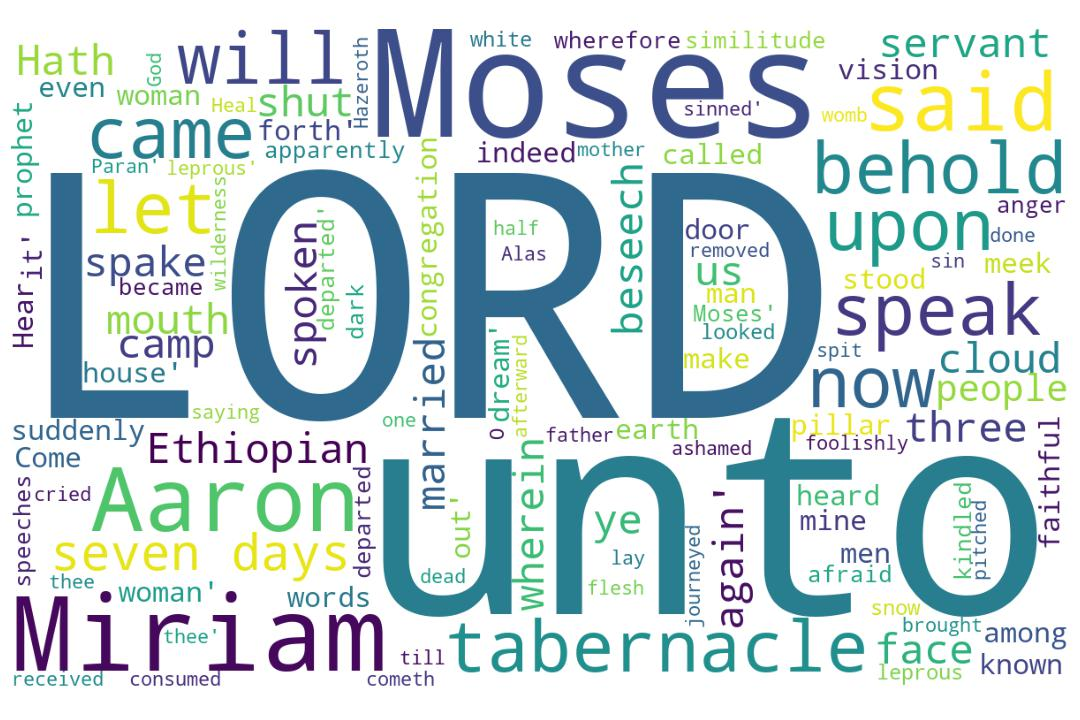
\includegraphics[width=\linewidth]{04OT-Numbers/Numbers12-WordCloud.jpg}
  \caption{Numbers 12 Word Cloud}
  \label{fig:Numbers 12 word Cloud}
\end{figure}

\marginpar{\scriptsize \centering \fcolorbox{bone}{lime}{\textbf{ABOUT THE LEADER}}\\ (Numbers 12:1-16) \begin{compactenum}[I.][8]
    \item \textbf{Authority Challenged} \index[scripture]{Numbers!Num 12:01}(Numbers 12:1)
    \item \textbf{Authenticity Confirmed} \index[scripture]{Numbers!Num 12:06--08}(Numbers 12:6-8)
    \item \textbf{Angered Kindled} \index[scripture]{Numbers!Num 12:10}(Numbers 12:10)
    \item \textbf{Arbitrated Clemency} \index[scripture]{Numbers!Num 12:14}(Numbers 12:14)
\end{compactenum}}


\footnote{\textcolor[cmyk]{0.99998,1,0,0}{\hyperlink{TOC}{Return to end of Table of Contents.}}}\footnote{\href{https://audiobible.com/bible/numbers_12.html}{\textcolor[cmyk]{0.99998,1,0,0}{Numbers 12 Audio}}}\textcolor[cmyk]{0.99998,1,0,0}{And Miriam and Aaron \fcolorbox{bone}{lime}{spake against} Moses because of the Ethiopian woman whom he had married: for he had married an Ethiopian woman.}
[2] \textcolor[cmyk]{0.99998,1,0,0}{And they said, Hath the LORD indeed spoken only by Moses? hath he not spoken also by us? And the LORD heard \emph{it}.}
[3] \textcolor[cmyk]{0.99998,1,0,0}{(Now the man Moses \emph{was} very meek, above all the men which \emph{were} upon the face of the earth.)}
[4] \textcolor[cmyk]{0.99998,1,0,0}{And the LORD spake suddenly unto Moses, and unto Aaron, and unto Miriam, Come out ye three unto the tabernacle of the congregation. And they three came out.}
[5] \textcolor[cmyk]{0.99998,1,0,0}{And the LORD came down in the pillar of the cloud, and stood \emph{in} the door of the tabernacle, and called Aaron and Miriam: and they both came forth.}
[6] \textcolor[cmyk]{0.99998,1,0,0}{And he said, \fcolorbox{bone}{lime}{Hear now} my words: If there be a prophet among you, \emph{I} the LORD will make myself known unto him in a vision, \emph{and} will speak unto him in a dream.}
[7] \textcolor[cmyk]{0.99998,1,0,0}{My servant Moses \emph{is} not so, who \emph{is} faithful in all mine house.}
[8] \textcolor[cmyk]{0.99998,1,0,0}{With him will I speak mouth to mouth, even apparently, and not in dark speeches; and the similitude of the LORD shall he behold: wherefore then were ye not afraid to speak against my servant Moses?}
[9] \textcolor[cmyk]{0.99998,1,0,0}{And the anger of the LORD was kindled against them; and he departed.}
[10] \textcolor[cmyk]{0.99998,1,0,0}{And the \fcolorbox{bone}{lime}{cloud departed} from off the tabernacle; and, behold, Miriam \emph{became} leprous, \emph{white} as snow: and Aaron looked upon Miriam, and, behold, \emph{she} \emph{was} leprous.}
[11] \textcolor[cmyk]{0.99998,1,0,0}{And Aaron said unto Moses, Alas, my lord, I beseech thee, lay not the sin upon us, wherein we have done foolishly, and wherein we have sinned.}
[12] \textcolor[cmyk]{0.99998,1,0,0}{Let her not be as one dead, of whom the flesh is half consumed when he cometh out of his mother's womb.}
[13] \textcolor[cmyk]{0.99998,1,0,0}{And Moses cried unto the LORD, saying, Heal her now, O God, I beseech thee.}\\
\\
\P \textcolor[cmyk]{0.99998,1,0,0}{And the LORD said unto Moses, If her father had but spit in her face, should she not be ashamed seven days? let her be shut out from the camp seven days, and \fcolorbox{bone}{lime}{after that} let her be received in \emph{again}.}
[15] \textcolor[cmyk]{0.99998,1,0,0}{And Miriam was shut out from the camp seven days: and the people journeyed not till Miriam was brought in \emph{again}.}
[16] \textcolor[cmyk]{0.99998,1,0,0}{And afterward the people removed from Hazeroth, and pitched in the wilderness of Paran.}
\index[NWIV]{23!Numbers!Num 12:1}\index[AWIP]{And!Numbers!Num 12:1}\index[AWIP]{Miriam!Numbers!Num 12:1}\index[AWIP]{and!Numbers!Num 12:1}\index[AWIP]{Aaron!Numbers!Num 12:1}\index[AWIP]{spake!Numbers!Num 12:1}\index[AWIP]{against!Numbers!Num 12:1}\index[AWIP]{Moses!Numbers!Num 12:1}\index[AWIP]{because!Numbers!Num 12:1}\index[AWIP]{of!Numbers!Num 12:1}\index[AWIP]{the!Numbers!Num 12:1}\index[AWIP]{Ethiopian!Numbers!Num 12:1}\index[AWIP]{Ethiopian!Numbers!Num 12:1 (2)}\index[AWIP]{woman!Numbers!Num 12:1}\index[AWIP]{woman!Numbers!Num 12:1 (2)}\index[AWIP]{whom!Numbers!Num 12:1}\index[AWIP]{he!Numbers!Num 12:1}\index[AWIP]{he!Numbers!Num 12:1 (2)}\index[AWIP]{had!Numbers!Num 12:1}\index[AWIP]{had!Numbers!Num 12:1 (2)}\index[AWIP]{married!Numbers!Num 12:1}\index[AWIP]{married!Numbers!Num 12:1 (2)}\index[AWIP]{for!Numbers!Num 12:1}\index[AWIP]{an!Numbers!Num 12:1}

\index[NWIV]{23!Numbers!Num 12:2}\index[AWIP]{And!Numbers!Num 12:2}\index[AWIP]{And!Numbers!Num 12:2 (2)}\index[AWIP]{they!Numbers!Num 12:2}\index[AWIP]{said!Numbers!Num 12:2}\index[AWIP]{Hath!Numbers!Num 12:2}\index[AWIP]{the!Numbers!Num 12:2}\index[AWIP]{the!Numbers!Num 12:2 (2)}\index[AWIP]{LORD!Numbers!Num 12:2}\index[AWIP]{LORD!Numbers!Num 12:2 (2)}\index[AWIP]{indeed!Numbers!Num 12:2}\index[AWIP]{spoken!Numbers!Num 12:2}\index[AWIP]{spoken!Numbers!Num 12:2 (2)}\index[AWIP]{only!Numbers!Num 12:2}\index[AWIP]{by!Numbers!Num 12:2}\index[AWIP]{by!Numbers!Num 12:2 (2)}\index[AWIP]{Moses?!Numbers!Num 12:2}\index[AWIP]{hath!Numbers!Num 12:2}\index[AWIP]{he!Numbers!Num 12:2}\index[AWIP]{not!Numbers!Num 12:2}\index[AWIP]{also!Numbers!Num 12:2}\index[AWIP]{us?!Numbers!Num 12:2}\index[AWIP]{heard!Numbers!Num 12:2}\index[AWIP]{\emph{it}!Numbers!Num 12:2}\index[AWIP]{\emph{it}!Numbers!Num 12:2}

\index[NWIV]{19!Numbers!Num 12:3}\index[AWIP]{(Now!Numbers!Num 12:3}\index[AWIP]{the!Numbers!Num 12:3}\index[AWIP]{the!Numbers!Num 12:3 (2)}\index[AWIP]{the!Numbers!Num 12:3 (3)}\index[AWIP]{the!Numbers!Num 12:3 (4)}\index[AWIP]{man!Numbers!Num 12:3}\index[AWIP]{Moses!Numbers!Num 12:3}\index[AWIP]{\emph{was}!Numbers!Num 12:3}\index[AWIP]{very!Numbers!Num 12:3}\index[AWIP]{meek!Numbers!Num 12:3}\index[AWIP]{above!Numbers!Num 12:3}\index[AWIP]{all!Numbers!Num 12:3}\index[AWIP]{men!Numbers!Num 12:3}\index[AWIP]{which!Numbers!Num 12:3}\index[AWIP]{\emph{were}!Numbers!Num 12:3}\index[AWIP]{upon!Numbers!Num 12:3}\index[AWIP]{face!Numbers!Num 12:3}\index[AWIP]{of!Numbers!Num 12:3}\index[AWIP]{earth)!Numbers!Num 12:3}\index[AWIP]{\emph{was}!Numbers!Num 12:3}\index[AWIP]{\emph{were}!Numbers!Num 12:3}

\index[NWIV]{28!Numbers!Num 12:4}\index[AWIP]{And!Numbers!Num 12:4}\index[AWIP]{And!Numbers!Num 12:4 (2)}\index[AWIP]{the!Numbers!Num 12:4}\index[AWIP]{the!Numbers!Num 12:4 (2)}\index[AWIP]{the!Numbers!Num 12:4 (3)}\index[AWIP]{LORD!Numbers!Num 12:4}\index[AWIP]{spake!Numbers!Num 12:4}\index[AWIP]{suddenly!Numbers!Num 12:4}\index[AWIP]{unto!Numbers!Num 12:4}\index[AWIP]{unto!Numbers!Num 12:4 (2)}\index[AWIP]{unto!Numbers!Num 12:4 (3)}\index[AWIP]{unto!Numbers!Num 12:4 (4)}\index[AWIP]{Moses!Numbers!Num 12:4}\index[AWIP]{and!Numbers!Num 12:4}\index[AWIP]{and!Numbers!Num 12:4 (2)}\index[AWIP]{Aaron!Numbers!Num 12:4}\index[AWIP]{Miriam!Numbers!Num 12:4}\index[AWIP]{Come!Numbers!Num 12:4}\index[AWIP]{out!Numbers!Num 12:4}\index[AWIP]{out!Numbers!Num 12:4 (2)}\index[AWIP]{ye!Numbers!Num 12:4}\index[AWIP]{three!Numbers!Num 12:4}\index[AWIP]{three!Numbers!Num 12:4 (2)}\index[AWIP]{tabernacle!Numbers!Num 12:4}\index[AWIP]{of!Numbers!Num 12:4}\index[AWIP]{congregation!Numbers!Num 12:4}\index[AWIP]{they!Numbers!Num 12:4}\index[AWIP]{came!Numbers!Num 12:4}

\index[NWIV]{29!Numbers!Num 12:5}\index[AWIP]{And!Numbers!Num 12:5}\index[AWIP]{the!Numbers!Num 12:5}\index[AWIP]{the!Numbers!Num 12:5 (2)}\index[AWIP]{the!Numbers!Num 12:5 (3)}\index[AWIP]{the!Numbers!Num 12:5 (4)}\index[AWIP]{the!Numbers!Num 12:5 (5)}\index[AWIP]{LORD!Numbers!Num 12:5}\index[AWIP]{came!Numbers!Num 12:5}\index[AWIP]{came!Numbers!Num 12:5 (2)}\index[AWIP]{down!Numbers!Num 12:5}\index[AWIP]{in!Numbers!Num 12:5}\index[AWIP]{pillar!Numbers!Num 12:5}\index[AWIP]{of!Numbers!Num 12:5}\index[AWIP]{of!Numbers!Num 12:5 (2)}\index[AWIP]{cloud!Numbers!Num 12:5}\index[AWIP]{and!Numbers!Num 12:5}\index[AWIP]{and!Numbers!Num 12:5 (2)}\index[AWIP]{and!Numbers!Num 12:5 (3)}\index[AWIP]{and!Numbers!Num 12:5 (4)}\index[AWIP]{stood!Numbers!Num 12:5}\index[AWIP]{\emph{in}!Numbers!Num 12:5}\index[AWIP]{door!Numbers!Num 12:5}\index[AWIP]{tabernacle!Numbers!Num 12:5}\index[AWIP]{called!Numbers!Num 12:5}\index[AWIP]{Aaron!Numbers!Num 12:5}\index[AWIP]{Miriam!Numbers!Num 12:5}\index[AWIP]{they!Numbers!Num 12:5}\index[AWIP]{both!Numbers!Num 12:5}\index[AWIP]{forth!Numbers!Num 12:5}\index[AWIP]{\emph{in}!Numbers!Num 12:5}

\index[NWIV]{34!Numbers!Num 12:6}\index[AWIP]{And!Numbers!Num 12:6}\index[AWIP]{he!Numbers!Num 12:6}\index[AWIP]{said!Numbers!Num 12:6}\index[AWIP]{Hear!Numbers!Num 12:6}\index[AWIP]{now!Numbers!Num 12:6}\index[AWIP]{my!Numbers!Num 12:6}\index[AWIP]{words!Numbers!Num 12:6}\index[AWIP]{If!Numbers!Num 12:6}\index[AWIP]{there!Numbers!Num 12:6}\index[AWIP]{be!Numbers!Num 12:6}\index[AWIP]{a!Numbers!Num 12:6}\index[AWIP]{a!Numbers!Num 12:6 (2)}\index[AWIP]{a!Numbers!Num 12:6 (3)}\index[AWIP]{prophet!Numbers!Num 12:6}\index[AWIP]{among!Numbers!Num 12:6}\index[AWIP]{you!Numbers!Num 12:6}\index[AWIP]{\emph{I}!Numbers!Num 12:6}\index[AWIP]{the!Numbers!Num 12:6}\index[AWIP]{LORD!Numbers!Num 12:6}\index[AWIP]{will!Numbers!Num 12:6}\index[AWIP]{will!Numbers!Num 12:6 (2)}\index[AWIP]{make!Numbers!Num 12:6}\index[AWIP]{myself!Numbers!Num 12:6}\index[AWIP]{known!Numbers!Num 12:6}\index[AWIP]{unto!Numbers!Num 12:6}\index[AWIP]{unto!Numbers!Num 12:6 (2)}\index[AWIP]{him!Numbers!Num 12:6}\index[AWIP]{him!Numbers!Num 12:6 (2)}\index[AWIP]{in!Numbers!Num 12:6}\index[AWIP]{in!Numbers!Num 12:6 (2)}\index[AWIP]{vision!Numbers!Num 12:6}\index[AWIP]{\emph{and}!Numbers!Num 12:6}\index[AWIP]{speak!Numbers!Num 12:6}\index[AWIP]{dream!Numbers!Num 12:6}\index[AWIP]{\emph{I}!Numbers!Num 12:6}\index[AWIP]{\emph{and}!Numbers!Num 12:6}

\index[NWIV]{13!Numbers!Num 12:7}\index[AWIP]{My!Numbers!Num 12:7}\index[AWIP]{servant!Numbers!Num 12:7}\index[AWIP]{Moses!Numbers!Num 12:7}\index[AWIP]{\emph{is}!Numbers!Num 12:7}\index[AWIP]{\emph{is}!Numbers!Num 12:7 (2)}\index[AWIP]{not!Numbers!Num 12:7}\index[AWIP]{so!Numbers!Num 12:7}\index[AWIP]{who!Numbers!Num 12:7}\index[AWIP]{faithful!Numbers!Num 12:7}\index[AWIP]{in!Numbers!Num 12:7}\index[AWIP]{all!Numbers!Num 12:7}\index[AWIP]{mine!Numbers!Num 12:7}\index[AWIP]{house!Numbers!Num 12:7}\index[AWIP]{\emph{is}!Numbers!Num 12:7}\index[AWIP]{\emph{is}!Numbers!Num 12:7 (2)}

\index[NWIV]{36!Numbers!Num 12:8}\index[AWIP]{With!Numbers!Num 12:8}\index[AWIP]{him!Numbers!Num 12:8}\index[AWIP]{will!Numbers!Num 12:8}\index[AWIP]{I!Numbers!Num 12:8}\index[AWIP]{speak!Numbers!Num 12:8}\index[AWIP]{speak!Numbers!Num 12:8 (2)}\index[AWIP]{mouth!Numbers!Num 12:8}\index[AWIP]{mouth!Numbers!Num 12:8 (2)}\index[AWIP]{to!Numbers!Num 12:8}\index[AWIP]{to!Numbers!Num 12:8 (2)}\index[AWIP]{even!Numbers!Num 12:8}\index[AWIP]{apparently!Numbers!Num 12:8}\index[AWIP]{and!Numbers!Num 12:8}\index[AWIP]{and!Numbers!Num 12:8 (2)}\index[AWIP]{not!Numbers!Num 12:8}\index[AWIP]{not!Numbers!Num 12:8 (2)}\index[AWIP]{in!Numbers!Num 12:8}\index[AWIP]{dark!Numbers!Num 12:8}\index[AWIP]{speeches!Numbers!Num 12:8}\index[AWIP]{the!Numbers!Num 12:8}\index[AWIP]{the!Numbers!Num 12:8 (2)}\index[AWIP]{similitude!Numbers!Num 12:8}\index[AWIP]{of!Numbers!Num 12:8}\index[AWIP]{LORD!Numbers!Num 12:8}\index[AWIP]{shall!Numbers!Num 12:8}\index[AWIP]{he!Numbers!Num 12:8}\index[AWIP]{behold!Numbers!Num 12:8}\index[AWIP]{wherefore!Numbers!Num 12:8}\index[AWIP]{then!Numbers!Num 12:8}\index[AWIP]{were!Numbers!Num 12:8}\index[AWIP]{ye!Numbers!Num 12:8}\index[AWIP]{afraid!Numbers!Num 12:8}\index[AWIP]{against!Numbers!Num 12:8}\index[AWIP]{my!Numbers!Num 12:8}\index[AWIP]{servant!Numbers!Num 12:8}\index[AWIP]{Moses?!Numbers!Num 12:8}

\index[NWIV]{13!Numbers!Num 12:9}\index[AWIP]{And!Numbers!Num 12:9}\index[AWIP]{the!Numbers!Num 12:9}\index[AWIP]{the!Numbers!Num 12:9 (2)}\index[AWIP]{anger!Numbers!Num 12:9}\index[AWIP]{of!Numbers!Num 12:9}\index[AWIP]{LORD!Numbers!Num 12:9}\index[AWIP]{was!Numbers!Num 12:9}\index[AWIP]{kindled!Numbers!Num 12:9}\index[AWIP]{against!Numbers!Num 12:9}\index[AWIP]{them!Numbers!Num 12:9}\index[AWIP]{and!Numbers!Num 12:9}\index[AWIP]{he!Numbers!Num 12:9}\index[AWIP]{departed!Numbers!Num 12:9}

\index[NWIV]{26!Numbers!Num 12:10}\index[AWIP]{And!Numbers!Num 12:10}\index[AWIP]{the!Numbers!Num 12:10}\index[AWIP]{the!Numbers!Num 12:10 (2)}\index[AWIP]{cloud!Numbers!Num 12:10}\index[AWIP]{departed!Numbers!Num 12:10}\index[AWIP]{from!Numbers!Num 12:10}\index[AWIP]{off!Numbers!Num 12:10}\index[AWIP]{tabernacle!Numbers!Num 12:10}\index[AWIP]{and!Numbers!Num 12:10}\index[AWIP]{and!Numbers!Num 12:10 (2)}\index[AWIP]{and!Numbers!Num 12:10 (3)}\index[AWIP]{behold!Numbers!Num 12:10}\index[AWIP]{behold!Numbers!Num 12:10 (2)}\index[AWIP]{Miriam!Numbers!Num 12:10}\index[AWIP]{Miriam!Numbers!Num 12:10 (2)}\index[AWIP]{\emph{became}!Numbers!Num 12:10}\index[AWIP]{leprous!Numbers!Num 12:10}\index[AWIP]{leprous!Numbers!Num 12:10 (2)}\index[AWIP]{\emph{white}!Numbers!Num 12:10}\index[AWIP]{as!Numbers!Num 12:10}\index[AWIP]{snow!Numbers!Num 12:10}\index[AWIP]{Aaron!Numbers!Num 12:10}\index[AWIP]{looked!Numbers!Num 12:10}\index[AWIP]{upon!Numbers!Num 12:10}\index[AWIP]{\emph{she}!Numbers!Num 12:10}\index[AWIP]{\emph{was}!Numbers!Num 12:10}\index[AWIP]{\emph{became}!Numbers!Num 12:10}\index[AWIP]{\emph{white}!Numbers!Num 12:10}\index[AWIP]{\emph{she}!Numbers!Num 12:10}\index[AWIP]{\emph{was}!Numbers!Num 12:10}

\index[NWIV]{27!Numbers!Num 12:11}\index[AWIP]{And!Numbers!Num 12:11}\index[AWIP]{Aaron!Numbers!Num 12:11}\index[AWIP]{said!Numbers!Num 12:11}\index[AWIP]{unto!Numbers!Num 12:11}\index[AWIP]{Moses!Numbers!Num 12:11}\index[AWIP]{Alas!Numbers!Num 12:11}\index[AWIP]{my!Numbers!Num 12:11}\index[AWIP]{lord!Numbers!Num 12:11}\index[AWIP]{I!Numbers!Num 12:11}\index[AWIP]{beseech!Numbers!Num 12:11}\index[AWIP]{thee!Numbers!Num 12:11}\index[AWIP]{lay!Numbers!Num 12:11}\index[AWIP]{not!Numbers!Num 12:11}\index[AWIP]{the!Numbers!Num 12:11}\index[AWIP]{sin!Numbers!Num 12:11}\index[AWIP]{upon!Numbers!Num 12:11}\index[AWIP]{us!Numbers!Num 12:11}\index[AWIP]{wherein!Numbers!Num 12:11}\index[AWIP]{wherein!Numbers!Num 12:11 (2)}\index[AWIP]{we!Numbers!Num 12:11}\index[AWIP]{we!Numbers!Num 12:11 (2)}\index[AWIP]{have!Numbers!Num 12:11}\index[AWIP]{have!Numbers!Num 12:11 (2)}\index[AWIP]{done!Numbers!Num 12:11}\index[AWIP]{foolishly!Numbers!Num 12:11}\index[AWIP]{and!Numbers!Num 12:11}\index[AWIP]{sinned!Numbers!Num 12:11}

\index[NWIV]{22!Numbers!Num 12:12}\index[AWIP]{Let!Numbers!Num 12:12}\index[AWIP]{her!Numbers!Num 12:12}\index[AWIP]{not!Numbers!Num 12:12}\index[AWIP]{be!Numbers!Num 12:12}\index[AWIP]{as!Numbers!Num 12:12}\index[AWIP]{one!Numbers!Num 12:12}\index[AWIP]{dead!Numbers!Num 12:12}\index[AWIP]{of!Numbers!Num 12:12}\index[AWIP]{of!Numbers!Num 12:12 (2)}\index[AWIP]{whom!Numbers!Num 12:12}\index[AWIP]{the!Numbers!Num 12:12}\index[AWIP]{flesh!Numbers!Num 12:12}\index[AWIP]{is!Numbers!Num 12:12}\index[AWIP]{half!Numbers!Num 12:12}\index[AWIP]{consumed!Numbers!Num 12:12}\index[AWIP]{when!Numbers!Num 12:12}\index[AWIP]{he!Numbers!Num 12:12}\index[AWIP]{cometh!Numbers!Num 12:12}\index[AWIP]{out!Numbers!Num 12:12}\index[AWIP]{his!Numbers!Num 12:12}\index[AWIP]{mother's!Numbers!Num 12:12}\index[AWIP]{womb!Numbers!Num 12:12}

\index[NWIV]{15!Numbers!Num 12:13}\index[AWIP]{And!Numbers!Num 12:13}\index[AWIP]{Moses!Numbers!Num 12:13}\index[AWIP]{cried!Numbers!Num 12:13}\index[AWIP]{unto!Numbers!Num 12:13}\index[AWIP]{the!Numbers!Num 12:13}\index[AWIP]{LORD!Numbers!Num 12:13}\index[AWIP]{saying!Numbers!Num 12:13}\index[AWIP]{Heal!Numbers!Num 12:13}\index[AWIP]{her!Numbers!Num 12:13}\index[AWIP]{now!Numbers!Num 12:13}\index[AWIP]{O!Numbers!Num 12:13}\index[AWIP]{God!Numbers!Num 12:13}\index[AWIP]{I!Numbers!Num 12:13}\index[AWIP]{beseech!Numbers!Num 12:13}\index[AWIP]{thee!Numbers!Num 12:13}

\index[NWIV]{41!Numbers!Num 12:14}\index[AWIP]{And!Numbers!Num 12:14}\index[AWIP]{the!Numbers!Num 12:14}\index[AWIP]{the!Numbers!Num 12:14 (2)}\index[AWIP]{LORD!Numbers!Num 12:14}\index[AWIP]{said!Numbers!Num 12:14}\index[AWIP]{unto!Numbers!Num 12:14}\index[AWIP]{Moses!Numbers!Num 12:14}\index[AWIP]{If!Numbers!Num 12:14}\index[AWIP]{her!Numbers!Num 12:14}\index[AWIP]{her!Numbers!Num 12:14 (2)}\index[AWIP]{her!Numbers!Num 12:14 (3)}\index[AWIP]{her!Numbers!Num 12:14 (4)}\index[AWIP]{father!Numbers!Num 12:14}\index[AWIP]{had!Numbers!Num 12:14}\index[AWIP]{but!Numbers!Num 12:14}\index[AWIP]{spit!Numbers!Num 12:14}\index[AWIP]{in!Numbers!Num 12:14}\index[AWIP]{in!Numbers!Num 12:14 (2)}\index[AWIP]{face!Numbers!Num 12:14}\index[AWIP]{should!Numbers!Num 12:14}\index[AWIP]{she!Numbers!Num 12:14}\index[AWIP]{not!Numbers!Num 12:14}\index[AWIP]{be!Numbers!Num 12:14}\index[AWIP]{be!Numbers!Num 12:14 (2)}\index[AWIP]{be!Numbers!Num 12:14 (3)}\index[AWIP]{ashamed!Numbers!Num 12:14}\index[AWIP]{seven!Numbers!Num 12:14}\index[AWIP]{seven!Numbers!Num 12:14 (2)}\index[AWIP]{days?!Numbers!Num 12:14}\index[AWIP]{let!Numbers!Num 12:14}\index[AWIP]{let!Numbers!Num 12:14 (2)}\index[AWIP]{shut!Numbers!Num 12:14}\index[AWIP]{out!Numbers!Num 12:14}\index[AWIP]{from!Numbers!Num 12:14}\index[AWIP]{camp!Numbers!Num 12:14}\index[AWIP]{days!Numbers!Num 12:14}\index[AWIP]{and!Numbers!Num 12:14}\index[AWIP]{after!Numbers!Num 12:14}\index[AWIP]{that!Numbers!Num 12:14}\index[AWIP]{received!Numbers!Num 12:14}\index[AWIP]{\emph{again}!Numbers!Num 12:14}\index[AWIP]{\emph{again}!Numbers!Num 12:14}

\index[NWIV]{21!Numbers!Num 12:15}\index[AWIP]{And!Numbers!Num 12:15}\index[AWIP]{Miriam!Numbers!Num 12:15}\index[AWIP]{Miriam!Numbers!Num 12:15 (2)}\index[AWIP]{was!Numbers!Num 12:15}\index[AWIP]{was!Numbers!Num 12:15 (2)}\index[AWIP]{shut!Numbers!Num 12:15}\index[AWIP]{out!Numbers!Num 12:15}\index[AWIP]{from!Numbers!Num 12:15}\index[AWIP]{the!Numbers!Num 12:15}\index[AWIP]{the!Numbers!Num 12:15 (2)}\index[AWIP]{camp!Numbers!Num 12:15}\index[AWIP]{seven!Numbers!Num 12:15}\index[AWIP]{days!Numbers!Num 12:15}\index[AWIP]{and!Numbers!Num 12:15}\index[AWIP]{people!Numbers!Num 12:15}\index[AWIP]{journeyed!Numbers!Num 12:15}\index[AWIP]{not!Numbers!Num 12:15}\index[AWIP]{till!Numbers!Num 12:15}\index[AWIP]{brought!Numbers!Num 12:15}\index[AWIP]{in!Numbers!Num 12:15}\index[AWIP]{\emph{again}!Numbers!Num 12:15}\index[AWIP]{\emph{again}!Numbers!Num 12:15}

\index[NWIV]{14!Numbers!Num 12:16}\index[AWIP]{And!Numbers!Num 12:16}\index[AWIP]{afterward!Numbers!Num 12:16}\index[AWIP]{the!Numbers!Num 12:16}\index[AWIP]{the!Numbers!Num 12:16 (2)}\index[AWIP]{people!Numbers!Num 12:16}\index[AWIP]{removed!Numbers!Num 12:16}\index[AWIP]{from!Numbers!Num 12:16}\index[AWIP]{Hazeroth!Numbers!Num 12:16}\index[AWIP]{and!Numbers!Num 12:16}\index[AWIP]{pitched!Numbers!Num 12:16}\index[AWIP]{in!Numbers!Num 12:16}\index[AWIP]{wilderness!Numbers!Num 12:16}\index[AWIP]{of!Numbers!Num 12:16}\index[AWIP]{Paran!Numbers!Num 12:16}


\section{Numbers 12 Outlines}

\subsection{My Outlines}

\subsubsection{Complaining about God's Appointed Leader}
\index[speaker]{Keith Anthony!Numbers 12 (Complaining about God's Appointed Leader)}
\index[series]{Numbers (Keith Anthony)!Numbers 12 (Complaining about God's Appointed Leader)}
\index[date]{2017/02/13!Numbers 12 (Complaining about God's Appointed Leader) (Keith Anthony)}
%\textbf{Source: }Inspired by Ruckman Commentary on Psalms.\\
%\textbf{Introduction: }Pslam 44 is clearly the period of the Great Tribulation, with Psalm 45 following as the Marriage of the Lamb takes place in Heaven (Esther 1--2).
\begin{compactenum}[I.][8]
    \item \textbf{Authority Challenged} \index[scripture]{Numbers!Num 12:01}(Numbers 12:1)
    \item \textbf{Authenticity Confirmed} \index[scripture]{Numbers!Num 12:06--08}(Numbers 12:6-8)
    \item \textbf{Angered Kindled} \index[scripture]{Numbers!Num 12:10}(Numbers 12:10)
    \item \textbf{Arbitrated Clemency} \index[scripture]{Numbers!Num 12:14}(Numbers 12:14)
\end{compactenum}


\subsection{Outlines from Others}
\section{Numbers 12 Comments}

\subsection{Numeric Nuggets}
\textbf{13: } Verse 7 has 13 words. Verse 16 has 13 unique words.

\chapter{Psalm 44}

\begin{figure}
  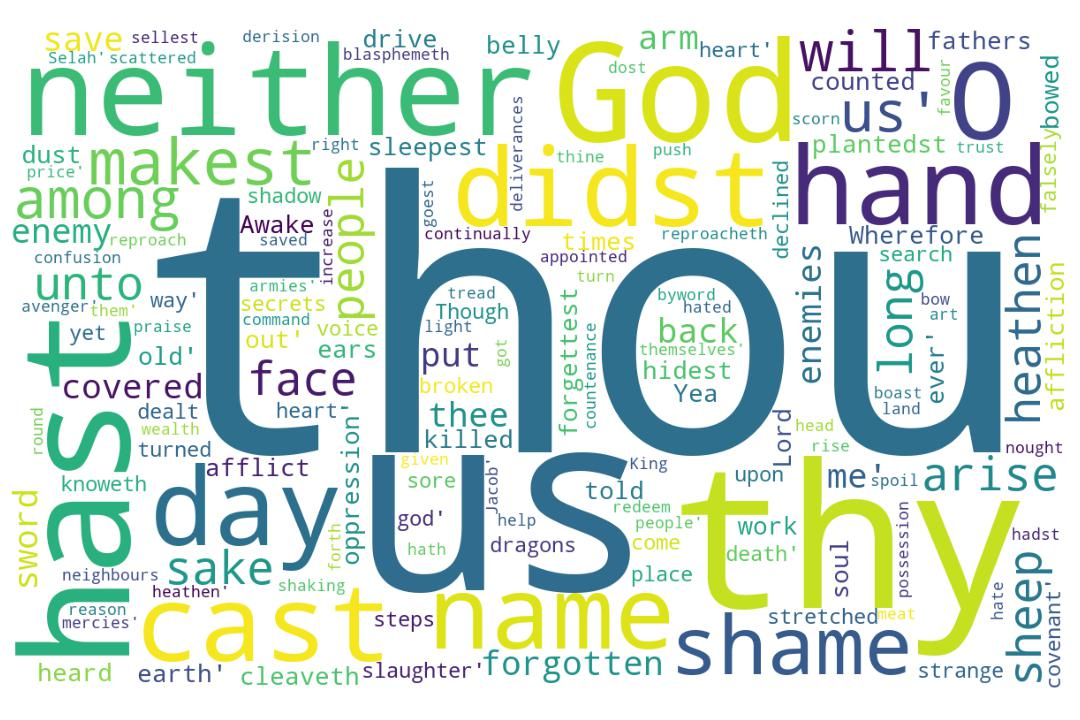
\includegraphics[width=\linewidth]{19OT-Psalms/Psalm44-WordCloud.jpg}
  \caption{Psalm 44 Word Cloud}
  \label{fig:Psalm 44 word Cloud}
\end{figure}

\marginpar{\scriptsize \centering \fcolorbox{bone}{lime}{\textbf{JACOB"S TROUBLES}}\\ (Psalm 44:1-26) \begin{compactenum}[I.][8]
    \item The \textbf{Son} of Perdition \index[scripture]{Psalms!Psa 044:01}(Psa 44:1)
    \item \textbf{Situation} Foretold %\index[scripture]{Exodus!Exodus 01:08}(Exodus 1:8)
    \item \textbf{Selah} Foretold \index[scripture]{Psalms!Psa 044:08}(Psa 44:8)
    \item Jews \textbf{Sacrificed} \index[scripture]{Psalms!Psa 044:11}\index[scripture]{Psalms!Psa 044:22}(Psa 44:11, 22)
    \item \textbf{Sold} into Slavery \index[scripture]{Psalms!Psa 044:12}(Psa 44:12)
    \item The \textbf{Shadow} of Death \index[scripture]{Psalms!Psa 044:23--24}(Psalm 44:23--24) (see also \index[scripture]{Exodus!Exo 01--03} Exodus 1--3, \index[scripture]{Job!Job 10:21--22}Job 10:21--22, \index[scripture]{Isaiah!Isa 09:02}Isa 9:2)
    \item The \textbf{Second} Advent Desired \index[scripture]{Psalms!Psa 044:26}(Psa 44:26)
\end{compactenum}}

\footnote{\textcolor[cmyk]{0.99998,1,0,0}{\hyperlink{TOC}{Return to end of Table of Contents.}}}\footnote{\href{https://www.audioverse.org/english/audiobibles/books/ENGKJV/O/Ps/1}{\textcolor[cmyk]{0.99998,1,0,0}{Psalms Audio}}}\textcolor[cmyk]{0.99998,1,0,0}{To the chief Musician for the sons of Korah, Maschil.}\\
\\
\textcolor[cmyk]{0.99998,1,0,0}{We have heard with our ears, O God, our fathers have told us, \emph{what} work thou didst in their days, in the times of old.}
[2] \textcolor[cmyk]{0.99998,1,0,0}{\emph{How} thou didst drive out the heathen with thy hand, and plantedst them; \emph{how} thou didst afflict the people, and cast them out.}\marginpar{\scriptsize people, place, plantedst , possession, praise, price, push, put}
[3] \textcolor[cmyk]{0.99998,1,0,0}{For they got not the land in possession by their own sword, neither did their own arm save them: but thy right hand, and thine arm, and the light of thy countenance, because thou hadst a favour unto them.}\marginpar{\scriptsize cast, cleaveth, come, command, confusion, continually, counted, countenance, covenant, covered}\footnote{\textbf{Exodus 15:6} - Thy right hand, O LORD, is become glorious in power: thy right hand, O LORD, hath dashed in pieces the enemy.}\footnote{\textbf{Exodus 15:12} -  Thou stretchedst out thy right hand, the earth swallowed them.}
[4] \textcolor[cmyk]{0.99998,1,0,0}{Thou art my King, O God: command deliverances for Jacob.}
[5] \textcolor[cmyk]{0.99998,1,0,0}{Through thee will we push down our enemies: through thy name will we tread them under that rise up against us.}
[6] \textcolor[cmyk]{0.99998,1,0,0}{For I will not trust in my bow, neither shall my sword save me.}
[7] \textcolor[cmyk]{0.99998,1,0,0}{But thou hast saved us from our enemies, and hast put them to shame that hated us.}
[8] \textcolor[cmyk]{0.99998,1,0,0}{In God we boast all the day long, and praise thy name for ever. \fcolorbox{bone}{lime}{Selah}.}\footnote{Compare with \textbf{Psalm 89:37-38} - It shall be established for ever as the moon, and as a faithful witness in heaven. Selah. [38] But thou hast cast off and abhorred, thou hast been wroth with thine anointed. Some things have to happen before the deliverances and triumphs spoken of in verses 4, 5, 7, and 8.} 
[9] \textcolor[cmyk]{0.99998,1,0,0}{But thou hast cast off, and put us to shame; and goest not forth with our armies.}
[10] \textcolor[cmyk]{0.99998,1,0,0}{Thou makest us to turn back from the enemy: and they which hate us spoil for themselves.}
[11] \textcolor[cmyk]{0.99998,1,0,0}{Thou hast given us like \fcolorbox{bone}{lime}{sheep \emph{appointed}} for meat; and hast \fcolorbox{bone}{lime}{scattered} us among the heathen.}\footnote{\textbf{Joel 3:2} -  I will also gather all nations, and will bring them down into the valley of Jehoshaphat, and will plead with them there for my people and for my heritage Israel, whom they have scattered among the nations, and parted my land.}
[12] \textcolor[cmyk]{0.99998,1,0,0}{Thou \fcolorbox{bone}{lime}{sellest} thy people for nought, and dost not increase \emph{thy} \emph{wealth} by their price.}\footnote{\textbf{Psalm 119:25} - My soul cleaveth unto the dust: quicken thou me according to thy word.}\footnote{\textbf{Lamentations 4:8} - Their visage is blacker than a coal; they are not known in the streets: their skin cleaveth to their bones; it is withered, it is become like a stick.}
[13] \textcolor[cmyk]{0.99998,1,0,0}{Thou makest us a reproach to our neighbours, a scorn and a derision to them that are round about us.}\footnote{\textbf{Job 30:1} - But now they that are younger than I have me in derision, whose fathers I would have disdained to have set with the dogs of my flock.}\footnote{\textbf{Psalm 79:4} -We are become a reproach to our neighbours, a scorn and derision to them that are round about us.}\footnote{\textbf{Psalm 119:51} - The proud have had me greatly in derision: yet have I not declined from thy law.}\footnote{\textbf{Ezekiel 36:4} - The proud have had me greatly in derision: yet have I not declined from thy law.}
[14] \textcolor[cmyk]{0.99998,1,0,0}{Thou makest us a byword among the heathen, a shaking of the head among the people.}\footnote{\textbf{Deuteronomy 28:38} - And now am I their song, yea, I am their byword.}\footnote{\textbf{Job 17:6} - He hath made me also a byword of the people; and aforetime I was as a tabret.}\footnote{\textbf{Job 30:9} - And now am I their song, yea, I am their byword.}
[15] \textcolor[cmyk]{0.99998,1,0,0}{My confusion \emph{is} continually before me, and the shame of my face hath covered me,}\footnote{\textbf{Ezra 9:7} - Since the days of our fathers have we been in a great trespass unto this day; and for our iniquities have we, our kings, and our priests, been delivered into the hand of the kings of the lands, to the sword, to captivity, and to a spoil, and to confusion of face, as it is this day.}\footnote{\textbf{Job 10:15} - If I be wicked, woe unto me; and if I be righteous, yet will I not lift up my head. I am full of confusion; therefore see thou mine affliction;}
[16] \textcolor[cmyk]{0.99998,1,0,0}{For the voice of him that reproacheth and blasphemeth; by reason of the enemy and avenger.}\footnote{\textbf{Psalm 8:2}  - Out of the mouth of babes and sucklings hast thou ordained strength because of thine enemies, that thou mightest still the enemy and the avenger.}
[17] \textcolor[cmyk]{0.99998,1,0,0}{All this is come upon us; yet have we not forgotten thee, neither have we dealt falsely in thy covenant.}
[18] \textcolor[cmyk]{0.99998,1,0,0}{Our heart is not turned back, neither have our steps declined from thy way;}
[19] \textcolor[cmyk]{0.99998,1,0,0}{Though thou hast sore broken us in the place of dragons, and covered us with the shadow of death.}\footnote{\textbf{Psalm 38:8} -  am feeble and sore broken: I have roared by reason of the disquietness of my heart.}
[20] \textcolor[cmyk]{0.99998,1,0,0}{If we have forgotten the name of our God, or stretched out our hands to a strange god;}
[21] \textcolor[cmyk]{0.99998,1,0,0}{Shall not God search this out? for he knoweth the secrets of the heart.}\footnote{\textbf{Jeremiah 17:10} -  I the LORD search the heart, I try the reins, even to give every man according to his ways, and according to the fruit of his doings.}\footnote{\textbf{1 Corinthians 14:25} - And thus are the secrets of his heart made manifest; and so falling down on his face he will worship God, and report that God is in you of a truth.}
[22] \textcolor[cmyk]{0.99998,1,0,0}{Yea, for thy sake are we killed all the day long; we are counted as sheep for the slaughter.}\footnote{\textbf{Jeremiah 12:3} - But thou, O LORD, knowest me: thou hast seen me, and tried mine heart toward thee: pull them out like sheep for the slaughter, and prepare them for the day of slaughter.}\footnote{\textbf{Romans 8:36} - As it is written, For thy sake we are killed all the day long; we are accounted as sheep for the slaughter.}
[23] \textcolor[cmyk]{0.99998,1,0,0}{Awake, why sleepest thou, O Lord? arise, cast \emph{us} not off for ever.}
[24] \textcolor[cmyk]{0.99998,1,0,0}{Wherefore hidest thou thy face, \emph{and} forgettest our affliction and our oppression?}\footnote{\textbf{Deuteronomy 26:7} - And when we cried unto the LORD God of our fathers, the LORD heard our voice, and looked on our affliction, and our labour, and our oppression:}\footnote{\textbf{Psalm 107:39} - Again, they are minished and brought low through oppression, affliction, and sorrow.}
[25] \textcolor[cmyk]{0.99998,1,0,0}{For our soul is bowed down to the dust: our belly cleaveth unto the earth.}\footnote{\textbf{Psalm 22:29} - All they that be fat upon earth shall eat and worship: all they that go down to the dust shall bow before him: and none can keep alive his own soul.}
[26] \textcolor[cmyk]{0.99998,1,0,0}{Arise for our help, and redeem us for thy mercies's sake.}\footnote{\textbf{Psalm 130:7-8} - Let Israel hope in the LORD: for with the LORD there is mercy, and with him is plenteous redemption. [8] And he shall redeem Israel from all his iniquities.}




\index[NWIV]{25!Psalms!Psa 44:1}\index[AWIP]{We!Psalms!Psa 44:1}\index[AWIP]{have!Psalms!Psa 44:1}\index[AWIP]{have!Psalms!Psa 44:1 (2)}\index[AWIP]{heard!Psalms!Psa 44:1}\index[AWIP]{with!Psalms!Psa 44:1}\index[AWIP]{our!Psalms!Psa 44:1}\index[AWIP]{our!Psalms!Psa 44:1 (2)}\index[AWIP]{ears!Psalms!Psa 44:1}\index[AWIP]{O!Psalms!Psa 44:1}\index[AWIP]{God!Psalms!Psa 44:1}\index[AWIP]{fathers!Psalms!Psa 44:1}\index[AWIP]{told!Psalms!Psa 44:1}\index[AWIP]{us!Psalms!Psa 44:1}\index[AWIP]{\emph{what}!Psalms!Psa 44:1}\index[AWIP]{work!Psalms!Psa 44:1}\index[AWIP]{thou!Psalms!Psa 44:1}\index[AWIP]{didst!Psalms!Psa 44:1}\index[AWIP]{in!Psalms!Psa 44:1}\index[AWIP]{in!Psalms!Psa 44:1 (2)}\index[AWIP]{their!Psalms!Psa 44:1}\index[AWIP]{days!Psalms!Psa 44:1}\index[AWIP]{the!Psalms!Psa 44:1}\index[AWIP]{times!Psalms!Psa 44:1}\index[AWIP]{of!Psalms!Psa 44:1}\index[AWIP]{old!Psalms!Psa 44:1}\index[AWIP]{\emph{what}!Psalms!Psa 44:1}

\index[NWIV]{23!Psalms!Psa 44:2}\index[AWIP]{\emph{How}!Psalms!Psa 44:2}\index[AWIP]{thou!Psalms!Psa 44:2}\index[AWIP]{thou!Psalms!Psa 44:2 (2)}\index[AWIP]{didst!Psalms!Psa 44:2}\index[AWIP]{didst!Psalms!Psa 44:2 (2)}\index[AWIP]{drive!Psalms!Psa 44:2}\index[AWIP]{out!Psalms!Psa 44:2}\index[AWIP]{out!Psalms!Psa 44:2 (2)}\index[AWIP]{the!Psalms!Psa 44:2}\index[AWIP]{the!Psalms!Psa 44:2 (2)}\index[AWIP]{heathen!Psalms!Psa 44:2}\index[AWIP]{with!Psalms!Psa 44:2}\index[AWIP]{thy!Psalms!Psa 44:2}\index[AWIP]{hand!Psalms!Psa 44:2}\index[AWIP]{and!Psalms!Psa 44:2}\index[AWIP]{and!Psalms!Psa 44:2 (2)}\index[AWIP]{plantedst!Psalms!Psa 44:2}\index[AWIP]{them!Psalms!Psa 44:2}\index[AWIP]{them!Psalms!Psa 44:2 (2)}\index[AWIP]{\emph{how}!Psalms!Psa 44:2}\index[AWIP]{afflict!Psalms!Psa 44:2}\index[AWIP]{people!Psalms!Psa 44:2}\index[AWIP]{cast!Psalms!Psa 44:2}\index[AWIP]{\emph{How}!Psalms!Psa 44:2}\index[AWIP]{\emph{how}!Psalms!Psa 44:2}

\index[NWIV]{39!Psalms!Psa 44:3}\index[AWIP]{For!Psalms!Psa 44:3}\index[AWIP]{they!Psalms!Psa 44:3}\index[AWIP]{got!Psalms!Psa 44:3}\index[AWIP]{not!Psalms!Psa 44:3}\index[AWIP]{the!Psalms!Psa 44:3}\index[AWIP]{the!Psalms!Psa 44:3 (2)}\index[AWIP]{land!Psalms!Psa 44:3}\index[AWIP]{in!Psalms!Psa 44:3}\index[AWIP]{possession!Psalms!Psa 44:3}\index[AWIP]{by!Psalms!Psa 44:3}\index[AWIP]{their!Psalms!Psa 44:3}\index[AWIP]{their!Psalms!Psa 44:3 (2)}\index[AWIP]{own!Psalms!Psa 44:3}\index[AWIP]{own!Psalms!Psa 44:3 (2)}\index[AWIP]{sword!Psalms!Psa 44:3}\index[AWIP]{neither!Psalms!Psa 44:3}\index[AWIP]{did!Psalms!Psa 44:3}\index[AWIP]{arm!Psalms!Psa 44:3}\index[AWIP]{arm!Psalms!Psa 44:3 (2)}\index[AWIP]{save!Psalms!Psa 44:3}\index[AWIP]{them!Psalms!Psa 44:3}\index[AWIP]{them!Psalms!Psa 44:3 (2)}\index[AWIP]{but!Psalms!Psa 44:3}\index[AWIP]{thy!Psalms!Psa 44:3}\index[AWIP]{thy!Psalms!Psa 44:3 (2)}\index[AWIP]{right!Psalms!Psa 44:3}\index[AWIP]{hand!Psalms!Psa 44:3}\index[AWIP]{and!Psalms!Psa 44:3}\index[AWIP]{and!Psalms!Psa 44:3 (2)}\index[AWIP]{thine!Psalms!Psa 44:3}\index[AWIP]{light!Psalms!Psa 44:3}\index[AWIP]{of!Psalms!Psa 44:3}\index[AWIP]{countenance!Psalms!Psa 44:3}\index[AWIP]{because!Psalms!Psa 44:3}\index[AWIP]{thou!Psalms!Psa 44:3}\index[AWIP]{hadst!Psalms!Psa 44:3}\index[AWIP]{a!Psalms!Psa 44:3}\index[AWIP]{favour!Psalms!Psa 44:3}\index[AWIP]{unto!Psalms!Psa 44:3}

\index[NWIV]{10!Psalms!Psa 44:4}\index[AWIP]{Thou!Psalms!Psa 44:4}\index[AWIP]{art!Psalms!Psa 44:4}\index[AWIP]{my!Psalms!Psa 44:4}\index[AWIP]{King!Psalms!Psa 44:4}\index[AWIP]{O!Psalms!Psa 44:4}\index[AWIP]{God!Psalms!Psa 44:4}\index[AWIP]{command!Psalms!Psa 44:4}\index[AWIP]{deliverances!Psalms!Psa 44:4}\index[AWIP]{for!Psalms!Psa 44:4}\index[AWIP]{Jacob!Psalms!Psa 44:4}

\index[NWIV]{21!Psalms!Psa 44:5}\index[AWIP]{Through!Psalms!Psa 44:5}\index[AWIP]{thee!Psalms!Psa 44:5}\index[AWIP]{will!Psalms!Psa 44:5}\index[AWIP]{will!Psalms!Psa 44:5 (2)}\index[AWIP]{we!Psalms!Psa 44:5}\index[AWIP]{we!Psalms!Psa 44:5 (2)}\index[AWIP]{push!Psalms!Psa 44:5}\index[AWIP]{down!Psalms!Psa 44:5}\index[AWIP]{our!Psalms!Psa 44:5}\index[AWIP]{enemies!Psalms!Psa 44:5}\index[AWIP]{through!Psalms!Psa 44:5}\index[AWIP]{thy!Psalms!Psa 44:5}\index[AWIP]{name!Psalms!Psa 44:5}\index[AWIP]{tread!Psalms!Psa 44:5}\index[AWIP]{them!Psalms!Psa 44:5}\index[AWIP]{under!Psalms!Psa 44:5}\index[AWIP]{that!Psalms!Psa 44:5}\index[AWIP]{rise!Psalms!Psa 44:5}\index[AWIP]{up!Psalms!Psa 44:5}\index[AWIP]{against!Psalms!Psa 44:5}\index[AWIP]{us!Psalms!Psa 44:5}

\index[NWIV]{14!Psalms!Psa 44:6}\index[AWIP]{For!Psalms!Psa 44:6}\index[AWIP]{I!Psalms!Psa 44:6}\index[AWIP]{will!Psalms!Psa 44:6}\index[AWIP]{not!Psalms!Psa 44:6}\index[AWIP]{trust!Psalms!Psa 44:6}\index[AWIP]{in!Psalms!Psa 44:6}\index[AWIP]{my!Psalms!Psa 44:6}\index[AWIP]{my!Psalms!Psa 44:6 (2)}\index[AWIP]{bow!Psalms!Psa 44:6}\index[AWIP]{neither!Psalms!Psa 44:6}\index[AWIP]{shall!Psalms!Psa 44:6}\index[AWIP]{sword!Psalms!Psa 44:6}\index[AWIP]{save!Psalms!Psa 44:6}\index[AWIP]{me!Psalms!Psa 44:6}

\index[NWIV]{17!Psalms!Psa 44:7}\index[AWIP]{But!Psalms!Psa 44:7}\index[AWIP]{thou!Psalms!Psa 44:7}\index[AWIP]{hast!Psalms!Psa 44:7}\index[AWIP]{hast!Psalms!Psa 44:7 (2)}\index[AWIP]{saved!Psalms!Psa 44:7}\index[AWIP]{us!Psalms!Psa 44:7}\index[AWIP]{us!Psalms!Psa 44:7 (2)}\index[AWIP]{from!Psalms!Psa 44:7}\index[AWIP]{our!Psalms!Psa 44:7}\index[AWIP]{enemies!Psalms!Psa 44:7}\index[AWIP]{and!Psalms!Psa 44:7}\index[AWIP]{put!Psalms!Psa 44:7}\index[AWIP]{them!Psalms!Psa 44:7}\index[AWIP]{to!Psalms!Psa 44:7}\index[AWIP]{shame!Psalms!Psa 44:7}\index[AWIP]{that!Psalms!Psa 44:7}\index[AWIP]{hated!Psalms!Psa 44:7}

\index[NWIV]{15!Psalms!Psa 44:8}\index[AWIP]{In!Psalms!Psa 44:8}\index[AWIP]{God!Psalms!Psa 44:8}\index[AWIP]{we!Psalms!Psa 44:8}\index[AWIP]{boast!Psalms!Psa 44:8}\index[AWIP]{all!Psalms!Psa 44:8}\index[AWIP]{the!Psalms!Psa 44:8}\index[AWIP]{day!Psalms!Psa 44:8}\index[AWIP]{long!Psalms!Psa 44:8}\index[AWIP]{and!Psalms!Psa 44:8}\index[AWIP]{praise!Psalms!Psa 44:8}\index[AWIP]{thy!Psalms!Psa 44:8}\index[AWIP]{name!Psalms!Psa 44:8}\index[AWIP]{for!Psalms!Psa 44:8}\index[AWIP]{ever!Psalms!Psa 44:8}\index[AWIP]{Selah!Psalms!Psa 44:8}

\index[NWIV]{17!Psalms!Psa 44:9}\index[AWIP]{But!Psalms!Psa 44:9}\index[AWIP]{thou!Psalms!Psa 44:9}\index[AWIP]{hast!Psalms!Psa 44:9}\index[AWIP]{cast!Psalms!Psa 44:9}\index[AWIP]{off!Psalms!Psa 44:9}\index[AWIP]{and!Psalms!Psa 44:9}\index[AWIP]{and!Psalms!Psa 44:9 (2)}\index[AWIP]{put!Psalms!Psa 44:9}\index[AWIP]{us!Psalms!Psa 44:9}\index[AWIP]{to!Psalms!Psa 44:9}\index[AWIP]{shame!Psalms!Psa 44:9}\index[AWIP]{goest!Psalms!Psa 44:9}\index[AWIP]{not!Psalms!Psa 44:9}\index[AWIP]{forth!Psalms!Psa 44:9}\index[AWIP]{with!Psalms!Psa 44:9}\index[AWIP]{our!Psalms!Psa 44:9}\index[AWIP]{armies!Psalms!Psa 44:9}

\index[NWIV]{17!Psalms!Psa 44:10}\index[AWIP]{Thou!Psalms!Psa 44:10}\index[AWIP]{makest!Psalms!Psa 44:10}\index[AWIP]{us!Psalms!Psa 44:10}\index[AWIP]{us!Psalms!Psa 44:10 (2)}\index[AWIP]{to!Psalms!Psa 44:10}\index[AWIP]{turn!Psalms!Psa 44:10}\index[AWIP]{back!Psalms!Psa 44:10}\index[AWIP]{from!Psalms!Psa 44:10}\index[AWIP]{the!Psalms!Psa 44:10}\index[AWIP]{enemy!Psalms!Psa 44:10}\index[AWIP]{and!Psalms!Psa 44:10}\index[AWIP]{they!Psalms!Psa 44:10}\index[AWIP]{which!Psalms!Psa 44:10}\index[AWIP]{hate!Psalms!Psa 44:10}\index[AWIP]{spoil!Psalms!Psa 44:10}\index[AWIP]{for!Psalms!Psa 44:10}\index[AWIP]{themselves!Psalms!Psa 44:10}

\index[NWIV]{16!Psalms!Psa 44:11}\index[AWIP]{Thou!Psalms!Psa 44:11}\index[AWIP]{hast!Psalms!Psa 44:11}\index[AWIP]{hast!Psalms!Psa 44:11 (2)}\index[AWIP]{given!Psalms!Psa 44:11}\index[AWIP]{us!Psalms!Psa 44:11}\index[AWIP]{us!Psalms!Psa 44:11 (2)}\index[AWIP]{like!Psalms!Psa 44:11}\index[AWIP]{sheep!Psalms!Psa 44:11}\index[AWIP]{\emph{appointed}!Psalms!Psa 44:11}\index[AWIP]{for!Psalms!Psa 44:11}\index[AWIP]{meat!Psalms!Psa 44:11}\index[AWIP]{and!Psalms!Psa 44:11}\index[AWIP]{scattered!Psalms!Psa 44:11}\index[AWIP]{among!Psalms!Psa 44:11}\index[AWIP]{the!Psalms!Psa 44:11}\index[AWIP]{heathen!Psalms!Psa 44:11}\index[AWIP]{\emph{appointed}!Psalms!Psa 44:11}

\index[NWIV]{15!Psalms!Psa 44:12}\index[AWIP]{Thou!Psalms!Psa 44:12}\index[AWIP]{sellest!Psalms!Psa 44:12}\index[AWIP]{thy!Psalms!Psa 44:12}\index[AWIP]{people!Psalms!Psa 44:12}\index[AWIP]{for!Psalms!Psa 44:12}\index[AWIP]{nought!Psalms!Psa 44:12}\index[AWIP]{and!Psalms!Psa 44:12}\index[AWIP]{dost!Psalms!Psa 44:12}\index[AWIP]{not!Psalms!Psa 44:12}\index[AWIP]{increase!Psalms!Psa 44:12}\index[AWIP]{\emph{thy}!Psalms!Psa 44:12}\index[AWIP]{\emph{wealth}!Psalms!Psa 44:12}\index[AWIP]{by!Psalms!Psa 44:12}\index[AWIP]{their!Psalms!Psa 44:12}\index[AWIP]{price!Psalms!Psa 44:12}\index[AWIP]{\emph{thy}!Psalms!Psa 44:12}\index[AWIP]{\emph{wealth}!Psalms!Psa 44:12}

\index[NWIV]{20!Psalms!Psa 44:13}\index[AWIP]{Thou!Psalms!Psa 44:13}\index[AWIP]{makest!Psalms!Psa 44:13}\index[AWIP]{us!Psalms!Psa 44:13}\index[AWIP]{us!Psalms!Psa 44:13 (2)}\index[AWIP]{a!Psalms!Psa 44:13}\index[AWIP]{a!Psalms!Psa 44:13 (2)}\index[AWIP]{a!Psalms!Psa 44:13 (3)}\index[AWIP]{reproach!Psalms!Psa 44:13}\index[AWIP]{to!Psalms!Psa 44:13}\index[AWIP]{to!Psalms!Psa 44:13 (2)}\index[AWIP]{our!Psalms!Psa 44:13}\index[AWIP]{neighbours!Psalms!Psa 44:13}\index[AWIP]{scorn!Psalms!Psa 44:13}\index[AWIP]{and!Psalms!Psa 44:13}\index[AWIP]{derision!Psalms!Psa 44:13}\index[AWIP]{them!Psalms!Psa 44:13}\index[AWIP]{that!Psalms!Psa 44:13}\index[AWIP]{are!Psalms!Psa 44:13}\index[AWIP]{round!Psalms!Psa 44:13}\index[AWIP]{about!Psalms!Psa 44:13}

\index[NWIV]{16!Psalms!Psa 44:14}\index[AWIP]{Thou!Psalms!Psa 44:14}\index[AWIP]{makest!Psalms!Psa 44:14}\index[AWIP]{us!Psalms!Psa 44:14}\index[AWIP]{a!Psalms!Psa 44:14}\index[AWIP]{a!Psalms!Psa 44:14 (2)}\index[AWIP]{byword!Psalms!Psa 44:14}\index[AWIP]{among!Psalms!Psa 44:14}\index[AWIP]{among!Psalms!Psa 44:14 (2)}\index[AWIP]{the!Psalms!Psa 44:14}\index[AWIP]{the!Psalms!Psa 44:14 (2)}\index[AWIP]{the!Psalms!Psa 44:14 (3)}\index[AWIP]{heathen!Psalms!Psa 44:14}\index[AWIP]{shaking!Psalms!Psa 44:14}\index[AWIP]{of!Psalms!Psa 44:14}\index[AWIP]{head!Psalms!Psa 44:14}\index[AWIP]{people!Psalms!Psa 44:14}

\index[NWIV]{15!Psalms!Psa 44:15}\index[AWIP]{My!Psalms!Psa 44:15}\index[AWIP]{confusion!Psalms!Psa 44:15}\index[AWIP]{\emph{is}!Psalms!Psa 44:15}\index[AWIP]{continually!Psalms!Psa 44:15}\index[AWIP]{before!Psalms!Psa 44:15}\index[AWIP]{me!Psalms!Psa 44:15}\index[AWIP]{me!Psalms!Psa 44:15 (2)}\index[AWIP]{and!Psalms!Psa 44:15}\index[AWIP]{the!Psalms!Psa 44:15}\index[AWIP]{shame!Psalms!Psa 44:15}\index[AWIP]{of!Psalms!Psa 44:15}\index[AWIP]{my!Psalms!Psa 44:15}\index[AWIP]{face!Psalms!Psa 44:15}\index[AWIP]{hath!Psalms!Psa 44:15}\index[AWIP]{covered!Psalms!Psa 44:15}\index[AWIP]{\emph{is}!Psalms!Psa 44:15}

\index[NWIV]{16!Psalms!Psa 44:16}\index[AWIP]{For!Psalms!Psa 44:16}\index[AWIP]{the!Psalms!Psa 44:16}\index[AWIP]{the!Psalms!Psa 44:16 (2)}\index[AWIP]{voice!Psalms!Psa 44:16}\index[AWIP]{of!Psalms!Psa 44:16}\index[AWIP]{of!Psalms!Psa 44:16 (2)}\index[AWIP]{him!Psalms!Psa 44:16}\index[AWIP]{that!Psalms!Psa 44:16}\index[AWIP]{reproacheth!Psalms!Psa 44:16}\index[AWIP]{and!Psalms!Psa 44:16}\index[AWIP]{and!Psalms!Psa 44:16 (2)}\index[AWIP]{blasphemeth!Psalms!Psa 44:16}\index[AWIP]{by!Psalms!Psa 44:16}\index[AWIP]{reason!Psalms!Psa 44:16}\index[AWIP]{enemy!Psalms!Psa 44:16}\index[AWIP]{avenger!Psalms!Psa 44:16}

\index[NWIV]{20!Psalms!Psa 44:17}\index[AWIP]{All!Psalms!Psa 44:17}\index[AWIP]{this!Psalms!Psa 44:17}\index[AWIP]{is!Psalms!Psa 44:17}\index[AWIP]{come!Psalms!Psa 44:17}\index[AWIP]{upon!Psalms!Psa 44:17}\index[AWIP]{us!Psalms!Psa 44:17}\index[AWIP]{yet!Psalms!Psa 44:17}\index[AWIP]{have!Psalms!Psa 44:17}\index[AWIP]{have!Psalms!Psa 44:17 (2)}\index[AWIP]{we!Psalms!Psa 44:17}\index[AWIP]{we!Psalms!Psa 44:17 (2)}\index[AWIP]{not!Psalms!Psa 44:17}\index[AWIP]{forgotten!Psalms!Psa 44:17}\index[AWIP]{thee!Psalms!Psa 44:17}\index[AWIP]{neither!Psalms!Psa 44:17}\index[AWIP]{dealt!Psalms!Psa 44:17}\index[AWIP]{falsely!Psalms!Psa 44:17}\index[AWIP]{in!Psalms!Psa 44:17}\index[AWIP]{thy!Psalms!Psa 44:17}\index[AWIP]{covenant!Psalms!Psa 44:17}

\index[NWIV]{14!Psalms!Psa 44:18}\index[AWIP]{Our!Psalms!Psa 44:18}\index[AWIP]{heart!Psalms!Psa 44:18}\index[AWIP]{is!Psalms!Psa 44:18}\index[AWIP]{not!Psalms!Psa 44:18}\index[AWIP]{turned!Psalms!Psa 44:18}\index[AWIP]{back!Psalms!Psa 44:18}\index[AWIP]{neither!Psalms!Psa 44:18}\index[AWIP]{have!Psalms!Psa 44:18}\index[AWIP]{our!Psalms!Psa 44:18}\index[AWIP]{steps!Psalms!Psa 44:18}\index[AWIP]{declined!Psalms!Psa 44:18}\index[AWIP]{from!Psalms!Psa 44:18}\index[AWIP]{thy!Psalms!Psa 44:18}\index[AWIP]{way!Psalms!Psa 44:18}

\index[NWIV]{19!Psalms!Psa 44:19}\index[AWIP]{Though!Psalms!Psa 44:19}\index[AWIP]{thou!Psalms!Psa 44:19}\index[AWIP]{hast!Psalms!Psa 44:19}\index[AWIP]{sore!Psalms!Psa 44:19}\index[AWIP]{broken!Psalms!Psa 44:19}\index[AWIP]{us!Psalms!Psa 44:19}\index[AWIP]{us!Psalms!Psa 44:19 (2)}\index[AWIP]{in!Psalms!Psa 44:19}\index[AWIP]{the!Psalms!Psa 44:19}\index[AWIP]{the!Psalms!Psa 44:19 (2)}\index[AWIP]{place!Psalms!Psa 44:19}\index[AWIP]{of!Psalms!Psa 44:19}\index[AWIP]{of!Psalms!Psa 44:19 (2)}\index[AWIP]{dragons!Psalms!Psa 44:19}\index[AWIP]{and!Psalms!Psa 44:19}\index[AWIP]{covered!Psalms!Psa 44:19}\index[AWIP]{with!Psalms!Psa 44:19}\index[AWIP]{shadow!Psalms!Psa 44:19}\index[AWIP]{death!Psalms!Psa 44:19}

\index[NWIV]{18!Psalms!Psa 44:20}\index[AWIP]{If!Psalms!Psa 44:20}\index[AWIP]{we!Psalms!Psa 44:20}\index[AWIP]{have!Psalms!Psa 44:20}\index[AWIP]{forgotten!Psalms!Psa 44:20}\index[AWIP]{the!Psalms!Psa 44:20}\index[AWIP]{name!Psalms!Psa 44:20}\index[AWIP]{of!Psalms!Psa 44:20}\index[AWIP]{our!Psalms!Psa 44:20}\index[AWIP]{our!Psalms!Psa 44:20 (2)}\index[AWIP]{God!Psalms!Psa 44:20}\index[AWIP]{or!Psalms!Psa 44:20}\index[AWIP]{stretched!Psalms!Psa 44:20}\index[AWIP]{out!Psalms!Psa 44:20}\index[AWIP]{hands!Psalms!Psa 44:20}\index[AWIP]{to!Psalms!Psa 44:20}\index[AWIP]{a!Psalms!Psa 44:20}\index[AWIP]{strange!Psalms!Psa 44:20}\index[AWIP]{god!Psalms!Psa 44:20}

\index[NWIV]{14!Psalms!Psa 44:21}\index[AWIP]{Shall!Psalms!Psa 44:21}\index[AWIP]{not!Psalms!Psa 44:21}\index[AWIP]{God!Psalms!Psa 44:21}\index[AWIP]{search!Psalms!Psa 44:21}\index[AWIP]{this!Psalms!Psa 44:21}\index[AWIP]{out?!Psalms!Psa 44:21}\index[AWIP]{for!Psalms!Psa 44:21}\index[AWIP]{he!Psalms!Psa 44:21}\index[AWIP]{knoweth!Psalms!Psa 44:21}\index[AWIP]{the!Psalms!Psa 44:21}\index[AWIP]{the!Psalms!Psa 44:21 (2)}\index[AWIP]{secrets!Psalms!Psa 44:21}\index[AWIP]{of!Psalms!Psa 44:21}\index[AWIP]{heart!Psalms!Psa 44:21}

\index[NWIV]{19!Psalms!Psa 44:22}\index[AWIP]{Yea!Psalms!Psa 44:22}\index[AWIP]{for!Psalms!Psa 44:22}\index[AWIP]{for!Psalms!Psa 44:22 (2)}\index[AWIP]{thy!Psalms!Psa 44:22}\index[AWIP]{sake!Psalms!Psa 44:22}\index[AWIP]{are!Psalms!Psa 44:22}\index[AWIP]{are!Psalms!Psa 44:22 (2)}\index[AWIP]{we!Psalms!Psa 44:22}\index[AWIP]{we!Psalms!Psa 44:22 (2)}\index[AWIP]{killed!Psalms!Psa 44:22}\index[AWIP]{all!Psalms!Psa 44:22}\index[AWIP]{the!Psalms!Psa 44:22}\index[AWIP]{the!Psalms!Psa 44:22 (2)}\index[AWIP]{day!Psalms!Psa 44:22}\index[AWIP]{long!Psalms!Psa 44:22}\index[AWIP]{counted!Psalms!Psa 44:22}\index[AWIP]{as!Psalms!Psa 44:22}\index[AWIP]{sheep!Psalms!Psa 44:22}\index[AWIP]{slaughter!Psalms!Psa 44:22}

\index[NWIV]{13!Psalms!Psa 44:23}\index[AWIP]{Awake!Psalms!Psa 44:23}\index[AWIP]{why!Psalms!Psa 44:23}\index[AWIP]{sleepest!Psalms!Psa 44:23}\index[AWIP]{thou!Psalms!Psa 44:23}\index[AWIP]{O!Psalms!Psa 44:23}\index[AWIP]{Lord?!Psalms!Psa 44:23}\index[AWIP]{arise!Psalms!Psa 44:23}\index[AWIP]{cast!Psalms!Psa 44:23}\index[AWIP]{\emph{us}!Psalms!Psa 44:23}\index[AWIP]{not!Psalms!Psa 44:23}\index[AWIP]{off!Psalms!Psa 44:23}\index[AWIP]{for!Psalms!Psa 44:23}\index[AWIP]{ever!Psalms!Psa 44:23}\index[AWIP]{\emph{us}!Psalms!Psa 44:23}

\index[NWIV]{12!Psalms!Psa 44:24}\index[AWIP]{Wherefore!Psalms!Psa 44:24}\index[AWIP]{hidest!Psalms!Psa 44:24}\index[AWIP]{thou!Psalms!Psa 44:24}\index[AWIP]{thy!Psalms!Psa 44:24}\index[AWIP]{face!Psalms!Psa 44:24}\index[AWIP]{\emph{and}!Psalms!Psa 44:24}\index[AWIP]{forgettest!Psalms!Psa 44:24}\index[AWIP]{our!Psalms!Psa 44:24}\index[AWIP]{our!Psalms!Psa 44:24 (2)}\index[AWIP]{affliction!Psalms!Psa 44:24}\index[AWIP]{and!Psalms!Psa 44:24}\index[AWIP]{oppression?!Psalms!Psa 44:24}\index[AWIP]{\emph{and}!Psalms!Psa 44:24}

\index[NWIV]{15!Psalms!Psa 44:25}\index[AWIP]{For!Psalms!Psa 44:25}\index[AWIP]{our!Psalms!Psa 44:25}\index[AWIP]{our!Psalms!Psa 44:25 (2)}\index[AWIP]{soul!Psalms!Psa 44:25}\index[AWIP]{is!Psalms!Psa 44:25}\index[AWIP]{bowed!Psalms!Psa 44:25}\index[AWIP]{down!Psalms!Psa 44:25}\index[AWIP]{to!Psalms!Psa 44:25}\index[AWIP]{the!Psalms!Psa 44:25}\index[AWIP]{the!Psalms!Psa 44:25 (2)}\index[AWIP]{dust!Psalms!Psa 44:25}\index[AWIP]{belly!Psalms!Psa 44:25}\index[AWIP]{cleaveth!Psalms!Psa 44:25}\index[AWIP]{unto!Psalms!Psa 44:25}\index[AWIP]{earth!Psalms!Psa 44:25}

\index[NWIV]{11!Psalms!Psa 44:26}\index[AWIP]{Arise!Psalms!Psa 44:26}\index[AWIP]{for!Psalms!Psa 44:26}\index[AWIP]{for!Psalms!Psa 44:26 (2)}\index[AWIP]{our!Psalms!Psa 44:26}\index[AWIP]{help!Psalms!Psa 44:26}\index[AWIP]{and!Psalms!Psa 44:26}\index[AWIP]{redeem!Psalms!Psa 44:26}\index[AWIP]{us!Psalms!Psa 44:26}\index[AWIP]{thy!Psalms!Psa 44:26}\index[AWIP]{mercies'!Psalms!Psa 44:26}\index[AWIP]{sake!Psalms!Psa 44:26}


\section{Psalm 44 Outlines}

\subsection{My Outlines}

\subsubsection{Jacob's Troubles}
\index[speaker]{Keith Anthony!Psalm 044 (Jacob's Troubles)}
\index[series]{Psalms (Keith Anthony)!Psalm 044 (Jacob's Troubles)}
\index[date]{2017/02/13!Psalm 044 (Jacob's Troubles) (Keith Anthony)}
\textbf{Source: }Inspired by Ruckman Commentary on Psalms.\\
\textbf{Introduction: }Psalm 44 is clearly the period of the Great Tribulation, with Psalm 45 following as the Marriage of the Lamb takes place in Heaven (Esther 1--2).

\begin{compactenum}[I.][7]
    \item The \textbf{Son} of Perdition \index[scripture]{Psalms!Psa 044:01}(Psa 44:1)
    \item \textbf{Situation} Foretold %\index[scripture]{Exodus!Exodus 01:08}(Exo 1:8)
    \item \textbf{Selah} Foretold \index[scripture]{Psalms!Psa 044:08}(Psa 44:8)
    \item Jews \textbf{Sacrificed} \index[scripture]{Psalms!Psa 044:11}\index[scripture]{Psalms!Psa 044:22}(Psa 44:11, 22)
    \item \textbf{Sold} into Slavery \index[scripture]{Psalms!Psa 044:12}(Psa 44:12)
    \item The \textbf{Shadow} of Death \index[scripture]{Psalms!Psa 044:23--24}(Psa 44:23--24) (see also \index[scripture]{Exodus!Exo 01--03}   \index[scripture]{Job!Job 10:21--22}  \index[scripture]{Isaiah!Isa 09:02} (Exo 1--3, Job 10:21--22, Isa 9:2)
    \item The \textbf{Second} Advent Desired \index[scripture]{Psalms!Psa 044:26}(Psa 44:26)
\end{compactenum}


\subsection{Outlines from Others}
\section{Psalm 44 Comments}
% cardinal red = \textcolor[cmyk]{0, 0.85. 0.70. 0.23}{}

\subsection{Numeric Nuggets}
\textbf{13: } Thirteen words are in verse 23.

\subsection{Psalm 44 Introduction}
The sense of the psalm is hinted at by several things.  It id, fist of all, a corporate psalm as evident by the use of plural nouns and pronouns. In its 26 verses, the word ``us'' is found 16 times and the word ``our'' 14 times. The word ``we'' is used 8 times. The capitalized ``We'' and ``Our'' are used once each. Then, there is a definite switch in content and tone between verses 8 and 9.  The ``collective'' goes from being at peace, with enemies subdued and secure in verse 8, to a  nation without a protector, on the run, and being bought and sold and literally consumed in verse 9.\\
\\
\noindent Its almost as if someone in whom they have trusted is suddenly revealed as an imposter and the group (God's covenant people) runs for the hills (see  Matthew 24:15).\footnote{\textbf{Matthew 24:15-16} -  \textcolor[cmyk]{0, 0.85. 0.70. 0.23}{When ye therefore shall see the abomination of desolation, spoken of by Daniel the prophet, stand in the holy place, (whoso readeth, let him understand:)} [16]  \textcolor[cmyk]{0, 0.85. 0.70. 0.23}{Then let them which be in Judaea flee into the mountains:} }

\subsection{Psalm 44:19}
See references to the ``shadow of death.'' (Job 3:5, Job 10:21, Job 10:22, Job 12:22, Job 16:16, Job 24:17 (2x) , Job 28:3, Job 34:22, Job 38:17, Psalms 23:4, Psalms 44:19, Psalms 107:10, Psalms 107:14,  Isaiah 9:2, Jeremiah 2:6, Jeremiah 13:16, Amos 5:8, Matthew 4:16, and Luke 1:79.) See modern corruptions of the verse discussed in Table~\ref{table:Corruption Psalm 44:19}.


\begin{center}

\begin{table}[ht]
\centering
\begin{tabular}{|p{.5in}|p{3.5in}|}
\hline

\textcolor[rgb]{0.00,0.00,1.00}{AV} & \textcolor[rgb]{0.00,0.00,1.00}{Though thou hast sore broken us in
the place of \textcolor[cmyk]{0, 0.85. 0.70. 0.23}{dragons}, and covered us with the \textcolor[cmyk]{0, 0.85. 0.70. 0.23}{shadow of death}.} \\ \hline 

\hline
\hline


ASV &  That thou hast sore broken us in the place of jackals, And covered us with the shadow of death.\\ \hline
CEB &  But you’ve crushed us in the place where jackals live,   covering us with deepest darkness.\\ \hline
ESV & yet you have broken us in the place of jackals   and covered us with the shadow of death.\\ \hline
NASV &  Yet You have crushed us in a place of jackals and covered us with the shadow of death. \\ \hline
MEV & though You have crushed us in the place of jackals,   and covered us with the shadow of death.\\ \hline
NIV &  But you crushed us and made us a haunt for jackals;  you covered us over with deep darkness. \\ \hline
NKJV &  But You have severely broken us in the place of jackals, And covered us with the shadow of death.\\ \hline
RSV &  that thou shouldst have broken us in the place of jackals,  and covered us with deep darkness.\\ \hline 

\hline
\hline

\multicolumn{2}{|p{4.3in}|}{{\textcolor{jungle}{Changing ``dragons' to ``jackal'' removes the connection to the ``great red dragon'' in Revelation 12:3, as well as all the cross references to ``dragon'' and ``dragons'' in scripture (35 uses in the AV). Further, truths about a creature known as Leviathan are also obscured (Job 41:1, Psalm 74:14, Psalm 104:26, and Isaiah 27:1 - note a total of FIVE references). Note that the very same word translated as ``dragon'' in the AV in Psalm 44:19 and NOT by modern versions, IS translated as ``dragon'' in modern versions in Isaiah 27:1.  Further, some of the modern versions replace ``shadow of death'' in the verse with ``deep darkness' (whatever ``deep darkness'' is.)}}} \\ \hline

\end{tabular}
\caption[Corruption Alert: Psalm 44:19]{Corruption Alert: Psalm 44:19} \label{table:Corruption Psalm 44:19}

\end{table}

\end{center}


%\newpage

%\begin{mdframed}[style=MyFrame]
%\begin{center}
%\begin{longtable}{|p{.5in}|p{3.5in}|}

%\caption[Corruption Alert: Psalm 44:19]{Corruption Alert: Psalm 44:19} \label{table:CorruptionPsalm 44:19} \\ 

%\hline  
%\multicolumn{1}{|c|}{\textbf{Version}} & 
%\multicolumn{1}{c|}{\textbf{Corruption}}  \\ \hline 
%\endfirsthead
 
%\multicolumn{2}{c}
%{{\bfseries \tablename\ \thetable{} -- continued from previous page}} \\  \hline  
%\multicolumn{1}{|c|}{\textbf{Version}} & 
%\multicolumn{1}{c|}{\textbf{Corruption}}  \\ \hline 
%\endhead
 
%\hline \multicolumn{2}{|r|}{{Continued on next page}} \\ \hline
%\endfoot 
%\textcolor[rgb]{0.00,0.00,1.00}{AV} & \textcolor[rgb]{0.00,0.00,1.00}{Though thou hast sore broken us in
%the place of \textcolor[cmyk]{0, 0.85. 0.70. 0.23}{dragons}, and covered us with the \textcolor[cmyk]{0, 0.85. 0.70. 0.23}{shadow of death}.} \\ \hline
%

%
% \multicolumn{2}{p{4.3in}}{{Changing ``dragons' to ``jackal'' removes the connection to the ``great red dragon'' in Revelation 12:3, as well as all the cross references to ``dragon'' and ``dragons'' in scripture (35 uses in the AV). Further, truths about a creature known as Leviathan are also obscured (Job 41:1, Psalm 74:14, Psalm 104:26, and Isaiah 27:1 - note a total of FIVE references). Note that the very same word translated as ``dragon'' in the AV in Psalm 44:19 and NOT by modern versions, IS translated as ``dragon'' in modern versions in Isaiah 27:1.  Further, some of the modern versions replace ``shadow of death'' in the verse with ``deep darkness' (whatever ``deep darkness'' is.)}} \\ %\hline

%\hline

%\end{longtable}
%\end{center}

%\normalsize 
%\end{mdframed}%

\chapter{Proverb 13}

\begin{figure}
  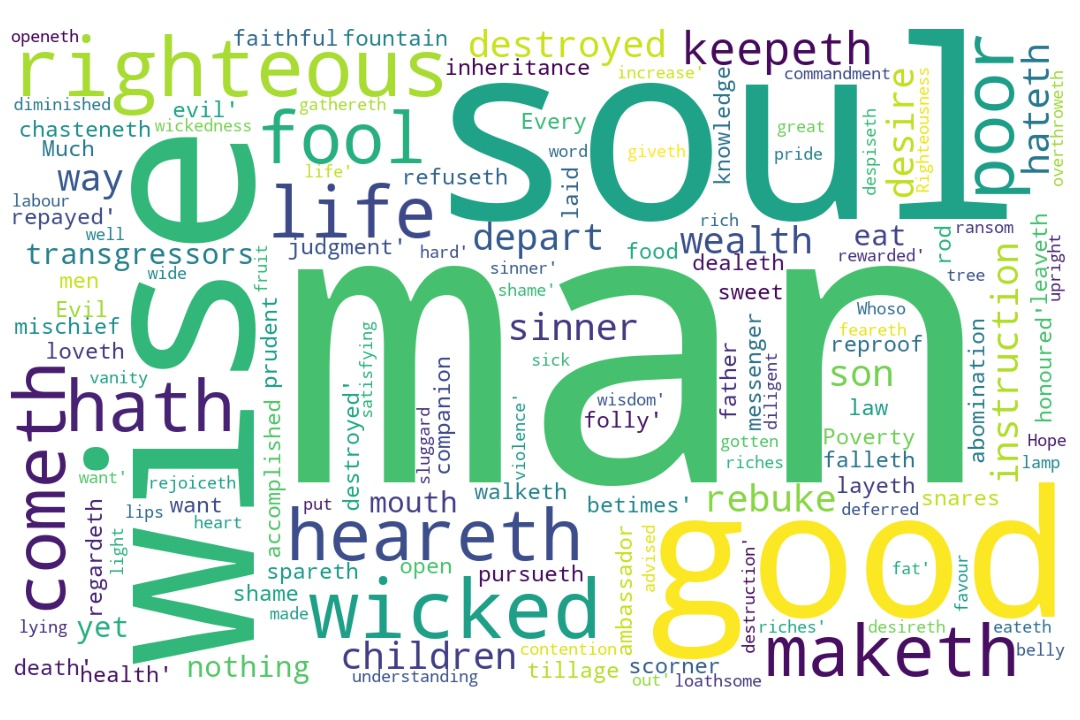
\includegraphics[width=\linewidth]{20OT-Proverbs/Proverb13-WordCloud.jpg}
  \caption{Proverb 13 Word Cloud}
  \label{fig:Proverb 13 Word Cloud}
\end{figure}

\marginpar{\scriptsize \centering \fcolorbox{bone}{lime}{\textbf{A WISE MAN}}\\ (Proverbs 13:1-25) \begin{compactenum}[I.][8]
    \item \textbf{Hears Instruction} \index[scripture]{Proverbs!Pro 13:01}(Pro 13:1)
    \item \textbf{Holds His Tongue} \index[scripture]{Proverbs!Pro 13:03}(Pro 13:3)
    \item \textbf{Hates Lying} \index[scripture]{Proverbs!Pro 13:05}(Pro 13:5)
    \item Is \textbf{Held up by Righteousness} \index[scripture]{Proverbs!Pro 13:06}(Pro 13:6)
    \item \textbf{Has True Wealth} \index[scripture]{Proverbs!Pro 13:07}(Pro 13:7)
    \item \textbf{Hearkens to God's Word} \index[scripture]{Proverbs!Pro 13:13}(Pro 13:13)
    \item \textbf{Hangs out with other wise Men} \index[scripture]{Proverbs!Pro 13:20}(Pro 13:20)
\end{compactenum}}

\marginpar{\scriptsize \centering \fcolorbox{bone}{yellow}{\textbf{A WISE SON}}\\ (Proverbs 13:1-25) \begin{compactenum}[I.][8]
    \item \textbf{Listens} to Instruction \index[scripture]{Proverbs!Pro 13:01}(Pro 13:1)
    \item \textbf{Learns}  \index[scripture]{Proverbs!Pro 13:01}(Pro 13:1)
    \item \textbf{Locks} his Lips \index[scripture]{Proverbs!Pro 13:03}(Pro 13:3)
    \item \textbf{Labours}  \index[scripture]{Proverbs!Pro 13:11}(Pro 13:11)
    \item \textbf{Likes} Reproof \index[scripture]{Proverbs!Pro 13:18}(Pro 13:18)
    \item \textbf{Leaves} an Inheritance \index[scripture]{Proverbs!Pro 13:22}(Pro 13:22)
    \item \textbf{Loves} Enough to Correct \index[scripture]{Proverbs!Pro 13:24}(Pro 13:24)
\end{compactenum}}

\footnote{\textcolor[cmyk]{0.99998,1,0,0}{\hyperlink{TOC}{Return to end of Table of Contents.}}}\footnote{\href{https://audiobible.com/bible/proverbs_13.html}{\textcolor[cmyk]{0.99998,1,0,0}{Proverbs Audio}}}\textcolor[cmyk]{0.99998,1,0,0}{A wise son \fcolorbox{bone}{lime}{\emph{heareth} his father's instruction}: but a scorner heareth not rebuke.}\footnote{\textbf{Isaiah 29:20} - For the terrible one is brought to nought, and the scorner is consumed, and all that watch for iniquity are cut off:}
[2] \textcolor[cmyk]{0.99998,1,0,0}{A man \fcolorbox{bone}{bone}{shall} eat good by the fruit of \emph{his} mouth: but the soul of the \fcolorbox{bone}{MYGOLD}{transgressors} \emph{\fcolorbox{bone}{bone}{shall}} \emph{eat} violence.}
[3] \textcolor[cmyk]{0.99998,1,0,0}{He that \fcolorbox{bone}{lime}{keepeth his mouth} keepeth his life: \emph{but} he that openeth wide his lips \fcolorbox{bone}{bone}{shall} have destruction.}
[4] \textcolor[cmyk]{0.99998,1,0,0}{The soul of the sluggard desireth, and \emph{hath} nothing: but the soul of the diligent \fcolorbox{bone}{bone}{shall} be made fat.}
[5] \textcolor[cmyk]{0.99998,1,0,0}{A righteous \emph{man} \fcolorbox{bone}{lime}{hateth lying}: but a wicked \emph{man} is loathsome, and cometh to shame.}
[6] \textcolor[cmyk]{0.99998,1,0,0}{\fcolorbox{bone}{MYGOLD}{Righteousness} keepeth \emph{him} \emph{that} \emph{is} upright in the way: but wickedness overthroweth the sinner.}
[7] \textcolor[cmyk]{0.99998,1,0,0}{There is that maketh himself rich, yet \emph{hath} nothing: \emph{there} \emph{is} that maketh himself poor, \fcolorbox{bone}{lime}{yet \emph{hath} great riches}.}
[8] \textcolor[cmyk]{0.99998,1,0,0}{The ransom of a man's life \emph{are} his riches: but the poor heareth not rebuke.}
[9] \textcolor[cmyk]{0.99998,1,0,0}{The light of the righteous rejoiceth: but the lamp of the wicked \fcolorbox{bone}{bone}{shall} be put out.}
[10] \textcolor[cmyk]{0.99998,1,0,0}{Only by pride cometh contention: but with the well advised \emph{is} wisdom.}
[11] \textcolor[cmyk]{0.99998,1,0,0}{Wealth \emph{gotten} by vanity \fcolorbox{bone}{bone}{shall} be diminished: but he that gathereth by labour \fcolorbox{bone}{bone}{shall} increase.}
[12] \textcolor[cmyk]{0.99998,1,0,0}{Hope deferred maketh the heart sick: but \emph{when} the desire cometh, \emph{it} \emph{is} a tree of life.}
[13] \textcolor[cmyk]{0.99998,1,0,0}{Whoso despiseth the word \fcolorbox{bone}{bone}{shall} be destroyed: but he that \fcolorbox{bone}{lime}{feareth the commandment} \fcolorbox{bone}{bone}{shall} be rewarded.}
[14] \textcolor[cmyk]{0.99998,1,0,0}{The law of the wise \emph{is} a fountain of life, to depart from the snares of death.}
[15] \textcolor[cmyk]{0.99998,1,0,0}{Good \fcolorbox{bone}{MYGOLD}{understanding} giveth favour: but the way of \fcolorbox{bone}{MYGOLD}{transgressors} \emph{is} hard.}
[16] \textcolor[cmyk]{0.99998,1,0,0}{Every prudent \emph{man} dealeth with knowledge: but a fool layeth open \emph{his} folly.}
[17] \textcolor[cmyk]{0.99998,1,0,0}{A wicked messenger falleth into mischief: but a faithful ambassador \emph{is} health.}
[18] \textcolor[cmyk]{0.99998,1,0,0}{Poverty and shame \emph{\fcolorbox{bone}{bone}{shall}} \emph{be} \emph{to} him that refuseth instruction: but he that regardeth reproof \fcolorbox{bone}{bone}{shall} be honoured.}
[19] \textcolor[cmyk]{0.99998,1,0,0}{The desire accomplished is sweet to the soul: but \emph{it} \emph{is} abomination to fools to depart from evil.}
[20] \textcolor[cmyk]{0.99998,1,0,0}{He that \fcolorbox{bone}{lime}{walketh with wise \emph{men}} \fcolorbox{bone}{bone}{shall} be wise: but a companion of fools \fcolorbox{bone}{bone}{shall} be destroyed.}\footnote{\textbf{2 Kings 9:11} - Then Jehu came forth to the servants of his lord: and one said unto him, Is all well? wherefore came this mad fellow to thee? And he said unto them, Ye know the man, and his communication.}\footnote{\textbf{1 Corinthians 15:33} - Be not deceived: evil communications corrupt good manners.}
[21] \textcolor[cmyk]{0.99998,1,0,0}{Evil pursueth sinners: but to the righteous good \fcolorbox{bone}{bone}{shall} be repayed.}
[22] \textcolor[cmyk]{0.99998,1,0,0}{A good \emph{man} leaveth an inheritance to his children's children: and the wealth of the sinner \emph{is} laid up for the just.}
[23] \textcolor[cmyk]{0.99998,1,0,0}{Much food \emph{is} \emph{in} the tillage of the poor: but there is \emph{that} \emph{is} destroyed for want of judgment.}
[24] \textcolor[cmyk]{0.99998,1,0,0}{He that spareth his rod hateth his son: but he that loveth him chasteneth him betimes.}
[25] \textcolor[cmyk]{0.99998,1,0,0}{The righteous eateth to the satisfying of his soul: but the belly of the wicked \fcolorbox{bone}{bone}{shall} want.}


% ransom , rebuke, refuseth, regardeth, rejoiceth, repayed, reproof, rewarded, rich, riches, righteous, rod

\index[NWIV]{13!Proverbs!Pro 13:1}\index[AWIP]{A!Proverbs!Pro 13:1}\index[AWIP]{wise!Proverbs!Pro 13:1}\index[AWIP]{son!Proverbs!Pro 13:1}\index[AWIP]{\emph{heareth}!Proverbs!Pro 13:1}\index[AWIP]{his!Proverbs!Pro 13:1}\index[AWIP]{father's!Proverbs!Pro 13:1}\index[AWIP]{instruction!Proverbs!Pro 13:1}\index[AWIP]{but!Proverbs!Pro 13:1}\index[AWIP]{a!Proverbs!Pro 13:1}\index[AWIP]{scorner!Proverbs!Pro 13:1}\index[AWIP]{heareth!Proverbs!Pro 13:1}\index[AWIP]{not!Proverbs!Pro 13:1}\index[AWIP]{rebuke!Proverbs!Pro 13:1}\index[AWIP]{\emph{heareth}!Proverbs!Pro 13:1}

\index[NWIV]{20!Proverbs!Pro 13:2}\index[AWIP]{A!Proverbs!Pro 13:2}\index[AWIP]{man!Proverbs!Pro 13:2}\index[AWIP]{shall!Proverbs!Pro 13:2}\index[AWIP]{eat!Proverbs!Pro 13:2}\index[AWIP]{good!Proverbs!Pro 13:2}\index[AWIP]{by!Proverbs!Pro 13:2}\index[AWIP]{the!Proverbs!Pro 13:2}\index[AWIP]{the!Proverbs!Pro 13:2 (2)}\index[AWIP]{the!Proverbs!Pro 13:2 (3)}\index[AWIP]{fruit!Proverbs!Pro 13:2}\index[AWIP]{of!Proverbs!Pro 13:2}\index[AWIP]{of!Proverbs!Pro 13:2 (2)}\index[AWIP]{\emph{his}!Proverbs!Pro 13:2}\index[AWIP]{mouth!Proverbs!Pro 13:2}\index[AWIP]{but!Proverbs!Pro 13:2}\index[AWIP]{soul!Proverbs!Pro 13:2}\index[AWIP]{transgressors!Proverbs!Pro 13:2}\index[AWIP]{\emph{shall}!Proverbs!Pro 13:2}\index[AWIP]{\emph{eat}!Proverbs!Pro 13:2}\index[AWIP]{violence!Proverbs!Pro 13:2}\index[AWIP]{\emph{his}!Proverbs!Pro 13:2}\index[AWIP]{\emph{shall}!Proverbs!Pro 13:2}\index[AWIP]{\emph{eat}!Proverbs!Pro 13:2}

\index[NWIV]{18!Proverbs!Pro 13:3}\index[AWIP]{He!Proverbs!Pro 13:3}\index[AWIP]{that!Proverbs!Pro 13:3}\index[AWIP]{that!Proverbs!Pro 13:3 (2)}\index[AWIP]{keepeth!Proverbs!Pro 13:3}\index[AWIP]{keepeth!Proverbs!Pro 13:3 (2)}\index[AWIP]{his!Proverbs!Pro 13:3}\index[AWIP]{his!Proverbs!Pro 13:3 (2)}\index[AWIP]{his!Proverbs!Pro 13:3 (3)}\index[AWIP]{mouth!Proverbs!Pro 13:3}\index[AWIP]{life!Proverbs!Pro 13:3}\index[AWIP]{\emph{but}!Proverbs!Pro 13:3}\index[AWIP]{he!Proverbs!Pro 13:3}\index[AWIP]{openeth!Proverbs!Pro 13:3}\index[AWIP]{wide!Proverbs!Pro 13:3}\index[AWIP]{lips!Proverbs!Pro 13:3}\index[AWIP]{shall!Proverbs!Pro 13:3}\index[AWIP]{have!Proverbs!Pro 13:3}\index[AWIP]{destruction!Proverbs!Pro 13:3}\index[AWIP]{\emph{but}!Proverbs!Pro 13:3}

\index[NWIV]{19!Proverbs!Pro 13:4}\index[AWIP]{The!Proverbs!Pro 13:4}\index[AWIP]{soul!Proverbs!Pro 13:4}\index[AWIP]{soul!Proverbs!Pro 13:4 (2)}\index[AWIP]{of!Proverbs!Pro 13:4}\index[AWIP]{of!Proverbs!Pro 13:4 (2)}\index[AWIP]{the!Proverbs!Pro 13:4}\index[AWIP]{the!Proverbs!Pro 13:4 (2)}\index[AWIP]{the!Proverbs!Pro 13:4 (3)}\index[AWIP]{sluggard!Proverbs!Pro 13:4}\index[AWIP]{desireth!Proverbs!Pro 13:4}\index[AWIP]{and!Proverbs!Pro 13:4}\index[AWIP]{\emph{hath}!Proverbs!Pro 13:4}\index[AWIP]{nothing!Proverbs!Pro 13:4}\index[AWIP]{but!Proverbs!Pro 13:4}\index[AWIP]{diligent!Proverbs!Pro 13:4}\index[AWIP]{shall!Proverbs!Pro 13:4}\index[AWIP]{be!Proverbs!Pro 13:4}\index[AWIP]{made!Proverbs!Pro 13:4}\index[AWIP]{fat!Proverbs!Pro 13:4}\index[AWIP]{\emph{hath}!Proverbs!Pro 13:4}

\index[NWIV]{15!Proverbs!Pro 13:5}\index[AWIP]{A!Proverbs!Pro 13:5}\index[AWIP]{righteous!Proverbs!Pro 13:5}\index[AWIP]{\emph{man}!Proverbs!Pro 13:5}\index[AWIP]{\emph{man}!Proverbs!Pro 13:5 (2)}\index[AWIP]{hateth!Proverbs!Pro 13:5}\index[AWIP]{lying!Proverbs!Pro 13:5}\index[AWIP]{but!Proverbs!Pro 13:5}\index[AWIP]{a!Proverbs!Pro 13:5}\index[AWIP]{wicked!Proverbs!Pro 13:5}\index[AWIP]{is!Proverbs!Pro 13:5}\index[AWIP]{loathsome!Proverbs!Pro 13:5}\index[AWIP]{and!Proverbs!Pro 13:5}\index[AWIP]{cometh!Proverbs!Pro 13:5}\index[AWIP]{to!Proverbs!Pro 13:5}\index[AWIP]{shame!Proverbs!Pro 13:5}\index[AWIP]{\emph{man}!Proverbs!Pro 13:5}\index[AWIP]{\emph{man}!Proverbs!Pro 13:5 (2)}

\index[NWIV]{14!Proverbs!Pro 13:6}\index[AWIP]{Righteousness!Proverbs!Pro 13:6}\index[AWIP]{keepeth!Proverbs!Pro 13:6}\index[AWIP]{\emph{him}!Proverbs!Pro 13:6}\index[AWIP]{\emph{that}!Proverbs!Pro 13:6}\index[AWIP]{\emph{is}!Proverbs!Pro 13:6}\index[AWIP]{upright!Proverbs!Pro 13:6}\index[AWIP]{in!Proverbs!Pro 13:6}\index[AWIP]{the!Proverbs!Pro 13:6}\index[AWIP]{the!Proverbs!Pro 13:6 (2)}\index[AWIP]{way!Proverbs!Pro 13:6}\index[AWIP]{but!Proverbs!Pro 13:6}\index[AWIP]{wickedness!Proverbs!Pro 13:6}\index[AWIP]{overthroweth!Proverbs!Pro 13:6}\index[AWIP]{sinner!Proverbs!Pro 13:6}\index[AWIP]{\emph{him}!Proverbs!Pro 13:6}\index[AWIP]{\emph{that}!Proverbs!Pro 13:6}\index[AWIP]{\emph{is}!Proverbs!Pro 13:6}

\index[NWIV]{19!Proverbs!Pro 13:7}\index[AWIP]{There!Proverbs!Pro 13:7}\index[AWIP]{is!Proverbs!Pro 13:7}\index[AWIP]{that!Proverbs!Pro 13:7}\index[AWIP]{that!Proverbs!Pro 13:7 (2)}\index[AWIP]{maketh!Proverbs!Pro 13:7}\index[AWIP]{maketh!Proverbs!Pro 13:7 (2)}\index[AWIP]{himself!Proverbs!Pro 13:7}\index[AWIP]{himself!Proverbs!Pro 13:7 (2)}\index[AWIP]{rich!Proverbs!Pro 13:7}\index[AWIP]{yet!Proverbs!Pro 13:7}\index[AWIP]{yet!Proverbs!Pro 13:7 (2)}\index[AWIP]{\emph{hath}!Proverbs!Pro 13:7}\index[AWIP]{\emph{hath}!Proverbs!Pro 13:7 (2)}\index[AWIP]{nothing!Proverbs!Pro 13:7}\index[AWIP]{\emph{there}!Proverbs!Pro 13:7}\index[AWIP]{\emph{is}!Proverbs!Pro 13:7}\index[AWIP]{poor!Proverbs!Pro 13:7}\index[AWIP]{great!Proverbs!Pro 13:7}\index[AWIP]{riches!Proverbs!Pro 13:7}\index[AWIP]{\emph{hath}!Proverbs!Pro 13:7}\index[AWIP]{\emph{hath}!Proverbs!Pro 13:7 (2)}\index[AWIP]{\emph{there}!Proverbs!Pro 13:7}\index[AWIP]{\emph{is}!Proverbs!Pro 13:7}

\index[NWIV]{15!Proverbs!Pro 13:8}\index[AWIP]{The!Proverbs!Pro 13:8}\index[AWIP]{ransom!Proverbs!Pro 13:8}\index[AWIP]{of!Proverbs!Pro 13:8}\index[AWIP]{a!Proverbs!Pro 13:8}\index[AWIP]{man's!Proverbs!Pro 13:8}\index[AWIP]{life!Proverbs!Pro 13:8}\index[AWIP]{\emph{are}!Proverbs!Pro 13:8}\index[AWIP]{his!Proverbs!Pro 13:8}\index[AWIP]{riches!Proverbs!Pro 13:8}\index[AWIP]{but!Proverbs!Pro 13:8}\index[AWIP]{the!Proverbs!Pro 13:8}\index[AWIP]{poor!Proverbs!Pro 13:8}\index[AWIP]{heareth!Proverbs!Pro 13:8}\index[AWIP]{not!Proverbs!Pro 13:8}\index[AWIP]{rebuke!Proverbs!Pro 13:8}\index[AWIP]{\emph{are}!Proverbs!Pro 13:8}

\index[NWIV]{16!Proverbs!Pro 13:9}\index[AWIP]{The!Proverbs!Pro 13:9}\index[AWIP]{light!Proverbs!Pro 13:9}\index[AWIP]{of!Proverbs!Pro 13:9}\index[AWIP]{of!Proverbs!Pro 13:9 (2)}\index[AWIP]{the!Proverbs!Pro 13:9}\index[AWIP]{the!Proverbs!Pro 13:9 (2)}\index[AWIP]{the!Proverbs!Pro 13:9 (3)}\index[AWIP]{righteous!Proverbs!Pro 13:9}\index[AWIP]{rejoiceth!Proverbs!Pro 13:9}\index[AWIP]{but!Proverbs!Pro 13:9}\index[AWIP]{lamp!Proverbs!Pro 13:9}\index[AWIP]{wicked!Proverbs!Pro 13:9}\index[AWIP]{shall!Proverbs!Pro 13:9}\index[AWIP]{be!Proverbs!Pro 13:9}\index[AWIP]{put!Proverbs!Pro 13:9}\index[AWIP]{out!Proverbs!Pro 13:9}

\index[NWIV]{12!Proverbs!Pro 13:10}\index[AWIP]{Only!Proverbs!Pro 13:10}\index[AWIP]{by!Proverbs!Pro 13:10}\index[AWIP]{pride!Proverbs!Pro 13:10}\index[AWIP]{cometh!Proverbs!Pro 13:10}\index[AWIP]{contention!Proverbs!Pro 13:10}\index[AWIP]{but!Proverbs!Pro 13:10}\index[AWIP]{with!Proverbs!Pro 13:10}\index[AWIP]{the!Proverbs!Pro 13:10}\index[AWIP]{well!Proverbs!Pro 13:10}\index[AWIP]{advised!Proverbs!Pro 13:10}\index[AWIP]{\emph{is}!Proverbs!Pro 13:10}\index[AWIP]{wisdom!Proverbs!Pro 13:10}\index[AWIP]{\emph{is}!Proverbs!Pro 13:10}

\index[NWIV]{15!Proverbs!Pro 13:11}\index[AWIP]{Wealth!Proverbs!Pro 13:11}\index[AWIP]{\emph{gotten}!Proverbs!Pro 13:11}\index[AWIP]{by!Proverbs!Pro 13:11}\index[AWIP]{by!Proverbs!Pro 13:11 (2)}\index[AWIP]{vanity!Proverbs!Pro 13:11}\index[AWIP]{shall!Proverbs!Pro 13:11}\index[AWIP]{shall!Proverbs!Pro 13:11 (2)}\index[AWIP]{be!Proverbs!Pro 13:11}\index[AWIP]{diminished!Proverbs!Pro 13:11}\index[AWIP]{but!Proverbs!Pro 13:11}\index[AWIP]{he!Proverbs!Pro 13:11}\index[AWIP]{that!Proverbs!Pro 13:11}\index[AWIP]{gathereth!Proverbs!Pro 13:11}\index[AWIP]{labour!Proverbs!Pro 13:11}\index[AWIP]{increase!Proverbs!Pro 13:11}\index[AWIP]{\emph{gotten}!Proverbs!Pro 13:11}

\index[NWIV]{17!Proverbs!Pro 13:12}\index[AWIP]{Hope!Proverbs!Pro 13:12}\index[AWIP]{deferred!Proverbs!Pro 13:12}\index[AWIP]{maketh!Proverbs!Pro 13:12}\index[AWIP]{the!Proverbs!Pro 13:12}\index[AWIP]{the!Proverbs!Pro 13:12 (2)}\index[AWIP]{heart!Proverbs!Pro 13:12}\index[AWIP]{sick!Proverbs!Pro 13:12}\index[AWIP]{but!Proverbs!Pro 13:12}\index[AWIP]{\emph{when}!Proverbs!Pro 13:12}\index[AWIP]{desire!Proverbs!Pro 13:12}\index[AWIP]{cometh!Proverbs!Pro 13:12}\index[AWIP]{\emph{it}!Proverbs!Pro 13:12}\index[AWIP]{\emph{is}!Proverbs!Pro 13:12}\index[AWIP]{a!Proverbs!Pro 13:12}\index[AWIP]{tree!Proverbs!Pro 13:12}\index[AWIP]{of!Proverbs!Pro 13:12}\index[AWIP]{life!Proverbs!Pro 13:12}\index[AWIP]{\emph{when}!Proverbs!Pro 13:12}\index[AWIP]{\emph{it}!Proverbs!Pro 13:12}\index[AWIP]{\emph{is}!Proverbs!Pro 13:12}

\index[NWIV]{16!Proverbs!Pro 13:13}\index[AWIP]{Whoso!Proverbs!Pro 13:13}\index[AWIP]{despiseth!Proverbs!Pro 13:13}\index[AWIP]{the!Proverbs!Pro 13:13}\index[AWIP]{the!Proverbs!Pro 13:13 (2)}\index[AWIP]{word!Proverbs!Pro 13:13}\index[AWIP]{shall!Proverbs!Pro 13:13}\index[AWIP]{shall!Proverbs!Pro 13:13 (2)}\index[AWIP]{be!Proverbs!Pro 13:13}\index[AWIP]{be!Proverbs!Pro 13:13 (2)}\index[AWIP]{destroyed!Proverbs!Pro 13:13}\index[AWIP]{but!Proverbs!Pro 13:13}\index[AWIP]{he!Proverbs!Pro 13:13}\index[AWIP]{that!Proverbs!Pro 13:13}\index[AWIP]{feareth!Proverbs!Pro 13:13}\index[AWIP]{commandment!Proverbs!Pro 13:13}\index[AWIP]{rewarded!Proverbs!Pro 13:13}

\index[NWIV]{17!Proverbs!Pro 13:14}\index[AWIP]{The!Proverbs!Pro 13:14}\index[AWIP]{law!Proverbs!Pro 13:14}\index[AWIP]{of!Proverbs!Pro 13:14}\index[AWIP]{of!Proverbs!Pro 13:14 (2)}\index[AWIP]{of!Proverbs!Pro 13:14 (3)}\index[AWIP]{the!Proverbs!Pro 13:14}\index[AWIP]{the!Proverbs!Pro 13:14 (2)}\index[AWIP]{wise!Proverbs!Pro 13:14}\index[AWIP]{\emph{is}!Proverbs!Pro 13:14}\index[AWIP]{a!Proverbs!Pro 13:14}\index[AWIP]{fountain!Proverbs!Pro 13:14}\index[AWIP]{life!Proverbs!Pro 13:14}\index[AWIP]{to!Proverbs!Pro 13:14}\index[AWIP]{depart!Proverbs!Pro 13:14}\index[AWIP]{from!Proverbs!Pro 13:14}\index[AWIP]{snares!Proverbs!Pro 13:14}\index[AWIP]{death!Proverbs!Pro 13:14}\index[AWIP]{\emph{is}!Proverbs!Pro 13:14}

\index[NWIV]{11!Proverbs!Pro 13:15}\index[AWIP]{Good!Proverbs!Pro 13:15}\index[AWIP]{understanding!Proverbs!Pro 13:15}\index[AWIP]{giveth!Proverbs!Pro 13:15}\index[AWIP]{favour!Proverbs!Pro 13:15}\index[AWIP]{but!Proverbs!Pro 13:15}\index[AWIP]{the!Proverbs!Pro 13:15}\index[AWIP]{way!Proverbs!Pro 13:15}\index[AWIP]{of!Proverbs!Pro 13:15}\index[AWIP]{transgressors!Proverbs!Pro 13:15}\index[AWIP]{\emph{is}!Proverbs!Pro 13:15}\index[AWIP]{hard!Proverbs!Pro 13:15}\index[AWIP]{\emph{is}!Proverbs!Pro 13:15}

\index[NWIV]{13!Proverbs!Pro 13:16}\index[AWIP]{Every!Proverbs!Pro 13:16}\index[AWIP]{prudent!Proverbs!Pro 13:16}\index[AWIP]{\emph{man}!Proverbs!Pro 13:16}\index[AWIP]{dealeth!Proverbs!Pro 13:16}\index[AWIP]{with!Proverbs!Pro 13:16}\index[AWIP]{knowledge!Proverbs!Pro 13:16}\index[AWIP]{but!Proverbs!Pro 13:16}\index[AWIP]{a!Proverbs!Pro 13:16}\index[AWIP]{fool!Proverbs!Pro 13:16}\index[AWIP]{layeth!Proverbs!Pro 13:16}\index[AWIP]{open!Proverbs!Pro 13:16}\index[AWIP]{\emph{his}!Proverbs!Pro 13:16}\index[AWIP]{folly!Proverbs!Pro 13:16}\index[AWIP]{\emph{man}!Proverbs!Pro 13:16}\index[AWIP]{\emph{his}!Proverbs!Pro 13:16}

\index[NWIV]{12!Proverbs!Pro 13:17}\index[AWIP]{A!Proverbs!Pro 13:17}\index[AWIP]{wicked!Proverbs!Pro 13:17}\index[AWIP]{messenger!Proverbs!Pro 13:17}\index[AWIP]{falleth!Proverbs!Pro 13:17}\index[AWIP]{into!Proverbs!Pro 13:17}\index[AWIP]{mischief!Proverbs!Pro 13:17}\index[AWIP]{but!Proverbs!Pro 13:17}\index[AWIP]{a!Proverbs!Pro 13:17}\index[AWIP]{faithful!Proverbs!Pro 13:17}\index[AWIP]{ambassador!Proverbs!Pro 13:17}\index[AWIP]{\emph{is}!Proverbs!Pro 13:17}\index[AWIP]{health!Proverbs!Pro 13:17}\index[AWIP]{\emph{is}!Proverbs!Pro 13:17}

\index[NWIV]{18!Proverbs!Pro 13:18}\index[AWIP]{Poverty!Proverbs!Pro 13:18}\index[AWIP]{and!Proverbs!Pro 13:18}\index[AWIP]{shame!Proverbs!Pro 13:18}\index[AWIP]{\emph{shall}!Proverbs!Pro 13:18}\index[AWIP]{\emph{be}!Proverbs!Pro 13:18}\index[AWIP]{\emph{to}!Proverbs!Pro 13:18}\index[AWIP]{him!Proverbs!Pro 13:18}\index[AWIP]{that!Proverbs!Pro 13:18}\index[AWIP]{that!Proverbs!Pro 13:18 (2)}\index[AWIP]{refuseth!Proverbs!Pro 13:18}\index[AWIP]{instruction!Proverbs!Pro 13:18}\index[AWIP]{but!Proverbs!Pro 13:18}\index[AWIP]{he!Proverbs!Pro 13:18}\index[AWIP]{regardeth!Proverbs!Pro 13:18}\index[AWIP]{reproof!Proverbs!Pro 13:18}\index[AWIP]{shall!Proverbs!Pro 13:18}\index[AWIP]{be!Proverbs!Pro 13:18}\index[AWIP]{honoured!Proverbs!Pro 13:18}\index[AWIP]{\emph{shall}!Proverbs!Pro 13:18}\index[AWIP]{\emph{be}!Proverbs!Pro 13:18}\index[AWIP]{\emph{to}!Proverbs!Pro 13:18}

\index[NWIV]{18!Proverbs!Pro 13:19}\index[AWIP]{The!Proverbs!Pro 13:19}\index[AWIP]{desire!Proverbs!Pro 13:19}\index[AWIP]{accomplished!Proverbs!Pro 13:19}\index[AWIP]{is!Proverbs!Pro 13:19}\index[AWIP]{sweet!Proverbs!Pro 13:19}\index[AWIP]{to!Proverbs!Pro 13:19}\index[AWIP]{to!Proverbs!Pro 13:19 (2)}\index[AWIP]{to!Proverbs!Pro 13:19 (3)}\index[AWIP]{the!Proverbs!Pro 13:19}\index[AWIP]{soul!Proverbs!Pro 13:19}\index[AWIP]{but!Proverbs!Pro 13:19}\index[AWIP]{\emph{it}!Proverbs!Pro 13:19}\index[AWIP]{\emph{is}!Proverbs!Pro 13:19}\index[AWIP]{abomination!Proverbs!Pro 13:19}\index[AWIP]{fools!Proverbs!Pro 13:19}\index[AWIP]{depart!Proverbs!Pro 13:19}\index[AWIP]{from!Proverbs!Pro 13:19}\index[AWIP]{evil!Proverbs!Pro 13:19}\index[AWIP]{\emph{it}!Proverbs!Pro 13:19}\index[AWIP]{\emph{is}!Proverbs!Pro 13:19}

\index[NWIV]{17!Proverbs!Pro 13:20}\index[AWIP]{He!Proverbs!Pro 13:20}\index[AWIP]{that!Proverbs!Pro 13:20}\index[AWIP]{walketh!Proverbs!Pro 13:20}\index[AWIP]{with!Proverbs!Pro 13:20}\index[AWIP]{wise!Proverbs!Pro 13:20}\index[AWIP]{wise!Proverbs!Pro 13:20 (2)}\index[AWIP]{\emph{men}!Proverbs!Pro 13:20}\index[AWIP]{shall!Proverbs!Pro 13:20}\index[AWIP]{shall!Proverbs!Pro 13:20 (2)}\index[AWIP]{be!Proverbs!Pro 13:20}\index[AWIP]{be!Proverbs!Pro 13:20 (2)}\index[AWIP]{but!Proverbs!Pro 13:20}\index[AWIP]{a!Proverbs!Pro 13:20}\index[AWIP]{companion!Proverbs!Pro 13:20}\index[AWIP]{of!Proverbs!Pro 13:20}\index[AWIP]{fools!Proverbs!Pro 13:20}\index[AWIP]{destroyed!Proverbs!Pro 13:20}\index[AWIP]{\emph{men}!Proverbs!Pro 13:20}

\index[NWIV]{11!Proverbs!Pro 13:21}\index[AWIP]{Evil!Proverbs!Pro 13:21}\index[AWIP]{pursueth!Proverbs!Pro 13:21}\index[AWIP]{sinners!Proverbs!Pro 13:21}\index[AWIP]{but!Proverbs!Pro 13:21}\index[AWIP]{to!Proverbs!Pro 13:21}\index[AWIP]{the!Proverbs!Pro 13:21}\index[AWIP]{righteous!Proverbs!Pro 13:21}\index[AWIP]{good!Proverbs!Pro 13:21}\index[AWIP]{shall!Proverbs!Pro 13:21}\index[AWIP]{be!Proverbs!Pro 13:21}\index[AWIP]{repayed!Proverbs!Pro 13:21}

\index[NWIV]{22!Proverbs!Pro 13:22}\index[AWIP]{A!Proverbs!Pro 13:22}\index[AWIP]{good!Proverbs!Pro 13:22}\index[AWIP]{\emph{man}!Proverbs!Pro 13:22}\index[AWIP]{leaveth!Proverbs!Pro 13:22}\index[AWIP]{an!Proverbs!Pro 13:22}\index[AWIP]{inheritance!Proverbs!Pro 13:22}\index[AWIP]{to!Proverbs!Pro 13:22}\index[AWIP]{his!Proverbs!Pro 13:22}\index[AWIP]{children's!Proverbs!Pro 13:22}\index[AWIP]{children!Proverbs!Pro 13:22}\index[AWIP]{and!Proverbs!Pro 13:22}\index[AWIP]{the!Proverbs!Pro 13:22}\index[AWIP]{the!Proverbs!Pro 13:22 (2)}\index[AWIP]{the!Proverbs!Pro 13:22 (3)}\index[AWIP]{wealth!Proverbs!Pro 13:22}\index[AWIP]{of!Proverbs!Pro 13:22}\index[AWIP]{sinner!Proverbs!Pro 13:22}\index[AWIP]{\emph{is}!Proverbs!Pro 13:22}\index[AWIP]{laid!Proverbs!Pro 13:22}\index[AWIP]{up!Proverbs!Pro 13:22}\index[AWIP]{for!Proverbs!Pro 13:22}\index[AWIP]{just!Proverbs!Pro 13:22}\index[AWIP]{\emph{man}!Proverbs!Pro 13:22}\index[AWIP]{\emph{is}!Proverbs!Pro 13:22}

\index[NWIV]{19!Proverbs!Pro 13:23}\index[AWIP]{Much!Proverbs!Pro 13:23}\index[AWIP]{food!Proverbs!Pro 13:23}\index[AWIP]{\emph{is}!Proverbs!Pro 13:23}\index[AWIP]{\emph{is}!Proverbs!Pro 13:23 (2)}\index[AWIP]{\emph{in}!Proverbs!Pro 13:23}\index[AWIP]{the!Proverbs!Pro 13:23}\index[AWIP]{the!Proverbs!Pro 13:23 (2)}\index[AWIP]{tillage!Proverbs!Pro 13:23}\index[AWIP]{of!Proverbs!Pro 13:23}\index[AWIP]{of!Proverbs!Pro 13:23 (2)}\index[AWIP]{poor!Proverbs!Pro 13:23}\index[AWIP]{but!Proverbs!Pro 13:23}\index[AWIP]{there!Proverbs!Pro 13:23}\index[AWIP]{is!Proverbs!Pro 13:23}\index[AWIP]{\emph{that}!Proverbs!Pro 13:23}\index[AWIP]{destroyed!Proverbs!Pro 13:23}\index[AWIP]{for!Proverbs!Pro 13:23}\index[AWIP]{want!Proverbs!Pro 13:23}\index[AWIP]{judgment!Proverbs!Pro 13:23}\index[AWIP]{\emph{is}!Proverbs!Pro 13:23}\index[AWIP]{\emph{is}!Proverbs!Pro 13:23 (2)}\index[AWIP]{\emph{in}!Proverbs!Pro 13:23}\index[AWIP]{\emph{that}!Proverbs!Pro 13:23}

\index[NWIV]{16!Proverbs!Pro 13:24}\index[AWIP]{He!Proverbs!Pro 13:24}\index[AWIP]{that!Proverbs!Pro 13:24}\index[AWIP]{that!Proverbs!Pro 13:24 (2)}\index[AWIP]{spareth!Proverbs!Pro 13:24}\index[AWIP]{his!Proverbs!Pro 13:24}\index[AWIP]{his!Proverbs!Pro 13:24 (2)}\index[AWIP]{rod!Proverbs!Pro 13:24}\index[AWIP]{hateth!Proverbs!Pro 13:24}\index[AWIP]{son!Proverbs!Pro 13:24}\index[AWIP]{but!Proverbs!Pro 13:24}\index[AWIP]{he!Proverbs!Pro 13:24}\index[AWIP]{loveth!Proverbs!Pro 13:24}\index[AWIP]{him!Proverbs!Pro 13:24}\index[AWIP]{him!Proverbs!Pro 13:24 (2)}\index[AWIP]{chasteneth!Proverbs!Pro 13:24}\index[AWIP]{betimes!Proverbs!Pro 13:24}

\index[NWIV]{17!Proverbs!Pro 13:25}\index[AWIP]{The!Proverbs!Pro 13:25}\index[AWIP]{righteous!Proverbs!Pro 13:25}\index[AWIP]{eateth!Proverbs!Pro 13:25}\index[AWIP]{to!Proverbs!Pro 13:25}\index[AWIP]{the!Proverbs!Pro 13:25}\index[AWIP]{the!Proverbs!Pro 13:25 (2)}\index[AWIP]{the!Proverbs!Pro 13:25 (3)}\index[AWIP]{satisfying!Proverbs!Pro 13:25}\index[AWIP]{of!Proverbs!Pro 13:25}\index[AWIP]{of!Proverbs!Pro 13:25 (2)}\index[AWIP]{his!Proverbs!Pro 13:25}\index[AWIP]{soul!Proverbs!Pro 13:25}\index[AWIP]{but!Proverbs!Pro 13:25}\index[AWIP]{belly!Proverbs!Pro 13:25}\index[AWIP]{wicked!Proverbs!Pro 13:25}\index[AWIP]{shall!Proverbs!Pro 13:25}\index[AWIP]{want!Proverbs!Pro 13:25}


\section{Proverb 13 Outlines}

\subsection{My Outlines}

\subsubsection{A Wise Man}

\index[speaker]{Keith Anthony!Proverb 13 (A Wise Man)}
\index[series]{Proverbs (Keith Anthony)!Pro 13 (A Wise Man)}
\index[date]{2016/05/13!Proverbs 13 (A Wise Man) (Keith Anthony)}
\begin{compactenum}[I.]
    \item \textbf{Hears Instruction} \index[scripture]{Proverbs!Pro 13:01}(Pro 13:1)
    \item \textbf{Holds His Tongue} \index[scripture]{Proverbs!Pro 13:03}(Pro 13:3)
    \item \textbf{Hates Lying} \index[scripture]{Proverbs!Pro 13:05}(Pro 13:5)
    \item Is \textbf{Help up by Righteousness} \index[scripture]{Proverbs!Pro 13:06}(Pro 13:6)
    \item \textbf{Has True Wealth} \index[scripture]{Proverbs!Pro 13:07}(Pro 13:7)
    \item \textbf{Hearkens to God's Word} \index[scripture]{Proverbs!Pro 13:13}(Pro 13:13)
    \item \textbf{Hangs out with other wise Men} \index[scripture]{Proverbs!Pro 13:20}(Pro 13:20)
\end{compactenum}

\subsubsection{A Wise Son}

\index[speaker]{Keith Anthony!Proverb 13 (A Wise Son)}
\index[series]{Proverbs (Keith Anthony)!Pro 13 (A Wise Son)}
\index[date]{2020/12/13!Proverbs 13 (A Wise Son) (Keith Anthony)}
 \begin{compactenum}[I.][8]
    \item \textbf{Listens} to Instruction \index[scripture]{Proverbs!Pro 13:01}(Pro 13:1)
    \item \textbf{Learns}  \index[scripture]{Proverbs!Pro 13:01}(Pro 13:1)
    \item \textbf{Locks} his Lips \index[scripture]{Proverbs!Pro 13:03}(Pro 13:3)
    \item \textbf{Labours}  \index[scripture]{Proverbs!Pro 13:11}(Pro 13:11)
    \item \textbf{Likes} Reproof \index[scripture]{Proverbs!Pro 13:18}(Pro 13:18)
    \item \textbf{Leaves} an Inheritance \index[scripture]{Proverbs!Pro 13:22}(Pro 13:22)
    \item \textbf{Loves} Enough to Correct \index[scripture]{Proverbs!Pro 13:24}(Pro 13:24)
\end{compactenum}

\subsection{Outlines from Others}

\section{Proverb 13 Comments}

\subsection{Numeric Nuggets}
\textbf{13:} Verses 1 and 16 have 13 words. Verses 1, 6, 9, 11, 13, 16, and 24 have 13 unique words. The word ``shall'' is found 13 times in the chapter.  The 13-letter words ``transgressors,'' ``Righteousness,'' and ``understanding'' are used in the cahpter.




%%% For Indexes

%\index[DEVOTIONAL]{TGIF1!Os Hillman (Living for a Cause Greater Than Yourself) - Proverb 19:17!2021/12/21}

%\index[DEVOTIONAL]{TGIF1!Os Hillman (Living for a Cause Greater Than Yourself) - Proverb 19:17!2021/12/21}

















%%% colour: cardinal red - \textcolor[cmyk]{0,0.85,0.70,0.23}{text}


%%%% Example marginpar with a compactenum list --- green color text
%\marginpar{\scriptsize \textcolor[rgb]{0.00,0.545,0.269}{$\rightarrow$7 Abominations: 
%\begin{compactenum}
%	\item A proud look,
%	\item a lying tongue,
%	\item hands that shed innocent blood,
%	\item An heart that deviseth wicked imaginations,
%	\item feet that be swift in running to mischief,
%	\item A false witness that speaketh lies, and
%	\item he that soweth discord among brethren.
%\end{compactenum}}}



%\newpage

%\begin{mdframed}[style=MyFrame]
%\begin{center}
%\begin{longtable}{|p{.5in}|p{3.5in}|}

%\caption[Corruption Alert: Proverbs 18:1]{Corruption Alert: Proverbs 18:1} \label{table:CorruptionProv18:1} \\ 

%\hline  
%\multicolumn{1}{|c|}{\textbf{Version}} & 
%\multicolumn{1}{c|}{\textbf{Corruption}}  \\ \hline 
%\endfirsthead
 
%\multicolumn{2}{c}
%{{\bfseries \tablename\ \thetable{} -- continued from previous page}} \\  \hline  
%\multicolumn{1}{|c|}{\textbf{Version}} & 
%\multicolumn{1}{c|}{\textbf{Corruption}}  \\ \hline 
%\endhead
 
%\hline \multicolumn{2}{|r|}{{Continued on next page}} \\ \hline
%\endfoot 
%\textcolor[rgb]{0.00,0.00,1.00}{AV} & \textcolor[rgb]{0.00,0.00,1.00}{Through desire a man, having separated himself, seeketh \emph{and} intermeddleth with all wisdom.} \\ \hline
%
%ASV &  He that separateth himself seeketh his own desire, And  rageth against all sound wisdom. \\ \hline
%
%CEB &  Unfriendly people look out for themselves; they bicker with sensible people.\\ \hline
%
%ESV & Whoever isolates himself seeks his own desire;  he breaks out against all sound judgment. \\ \hline
%
%NASV &  He who separates himself seeks his own desire, He quarrels against all sound wisdom.\\ \hline
%
%MEV & He who separates himself seeks his own desire; he seeks and quarrels against all wisdom.\\ \hline
%
%NIV &  An unfriendly person pursues selfish ends and against all sound judgment starts quarrels. \\ \hline
%
%NKJV &  A man who isolates himself seeks his own desire; He rages against all wise judgment.\\ \hline
%
%RSV &  He who is estranged seeks pretexts  to break out against all sound judgment.\\ \hline

% \multicolumn{2}{p{4.3in}}{{Modern translations, such as the ASV and others, strike out the first part of the verse, concealing the intent of mankind in genewisdom clearly revealed in scripture. How wonderful is the obfuscated RSV text: ``He who is estranged seeks pretexts.'' What does THAT mean?}} \\ %\hline

%\hline

%\end{longtable}
%\end{center}

%\normalsize 
%\end{mdframed}

%\marginpar{\scriptsize \centering \fcolorbox{black}{lime}{\textbf{OUTIDE THE PLACE OF PROMISE}}\\ (Psalm 137:1--9) 
%\begin{compactenum}[I.][8]
%	\item \textbf{Plight \& Distress} \index[scripture]{Psalms!Psa 137:01} (Psalm 137:1)
%	\item The \textbf{Place Desired} \index[scripture]{Psalms!Psa 137:01} (Psalm 137:1)
%	\item \textbf{Pining \& Despiar} \index[scripture]{Psalms!Psa 137:02} (Psalm 137:2)
%	\item \textbf{Provoked \& Degraded}\index[scripture]{Psalms!Psa 137:03} (Psalm 137:3)
%	\item The \textbf{Predicament Described}\index[scripture]{Psalms!Psa 137:04} (Psalm 137:4)
%	\item A \textbf{Preference Decided}\index[scripture]{Psalms!Psa 137:06} (Psalm 137:6)
%	\item A \textbf{Prediction of Destruction}\index[scripture]{Psalms!Psa 137:08} (Psalm 137:8)
%\end{compactenum} }


%\subsection{Outlines from Others}

%\subsubsection{Words on Wisdom}
%\index[speaker]{John Battles!Proverbs 01 (Words on Wisdom)}
%\index[series]{Proverbs (John Battles)!Proverbs 01 (Words on Wisdom)}
%\index[date]{2016/01/20!Proverbs 01 (Words on Wisdom) (John Battles)}
%\textbf{Lineage}: adpated from S. Conway\\
%\textbf{Introduction}: Proverbs distinctly points out things that a fool does:
%\begin{compactenum}[I.][4]
%	\item \textbf{Welcome to Wisdom} \index[scripture]{Proverbs!Pro 01:01-09}(Proverbs 1:1-9)
%	\item \textbf{Warnings of Wisdom} \index[scripture]{Proverbs!Pro 01:10-19}(Proverbs 1:10-19).
%	\item \textbf{Woe of Wisdom} \index[scripture]{Proverbs!Pro 01:24-32}(Proverbs 1:24-32)
%	\item \textbf{Watchcare of Wisdom} \index[scripture]{Proverbs!Pro 01:33}(Proverbs 1:33).
%\end{compactenum}


%%%%% COLOR FOR MARGINPAR OUTLINES
%% 1  LIME - \marginpar{\scriptsize \centering \fcolorbox{black}{lime}{\textbf{TITLE}}\\ (Passage) 
%% 2. YELLOW - \marginpar{\scriptsize \centering \fcolorbox{black}{yellow}{\textbf{TITLE}}\\ (Passage) 
%% 3. Blue BGND, WHITE LETTERS - \marginpar{\scriptsize \centering \fcolorbox{black}{blue}{\textbf{\textcolor[cmyk]{0,0,0,0}{TITLE}}}\\ (Passage) 
%% 4. black BGND, WHITE LETTERS - \marginpar{\scriptsize \centering \fcolorbox{black}{black}{\textbf{\textcolor[cmyk]{0,0,0,0}{TITLE}}}\\ (Passage) 
%% 5. red BGND, WHITE LETTERS - \marginpar{\scriptsize \centering \fcolorbox{black}{red}{\textbf{\textcolor[cmyk]{0,0,0,0}{TITLE}}}\\ (Passage) 

%%%%%% INCLUSION OF GRAPHIC
%\newpage

%\begin{figure}
%\begin{center}
%\includegraphics[scale=0.5, angle=90]{07OT-Judges/References/b201107i1-large}
%\caption[Summary of the 13 Judges]{Summary of the 13 Judges}
%\label{fig:Summary of the 13 Judges}
%\end{center}
%\end{figure}


%%%%%%%%%%%
%%%%%%%%%%%

% SYTEMATIC THEOLOGY (10 + 2)
% Theology proper – The study of the character of God
% Angelology – The study of angels
% Biblical theology – The study of the Bible
% Christology – The study of Christ
% Ecclesiology – The study of the church
% Eschatology – The study of the end times[5]
% Hamartiology – The study of sin
% Pneumatology – The study of the Holy Spirit
% Soteriology – The study of salvation
% Theological anthropology – The study of the nature of humanity.
% ++
% Moral theology
% Bilical cosomolgy

%%%%%%%%%%%%%%
%%%%%%%%%%%%%%

% \footnote{\href{https://audiobible.com/bible/psalms_91.html}{\textcolor[cmyk]{0.99998,1,0,0}{Psalm 91 Audio}}}

% \marginpar{\scriptsize \centering \fcolorbox{black}{lime}{\textbf{JERUSALEM}}\\
% \fcolorbox{black}{lime}{\textbf{DON'T GO BACK TO EGYPT}} \\ (Isaiah 31:1--9) 

%%%%%%%%%%%%%%
%%% Extra Colors
%%% from https://latexcolor.blogspot.com/2019/10/list-of-latex-colors.html
%%%%%%%%%%%%%%
% \definecolor{champagne}{rgb}{0.97,0.91,0.81}
% \definecolor{bone}{rgb}{0.89,0.85,0.79}
%\titleJE
%

%%%%% EXAMPLE Index entry:
% \index[DOCTRINES]{Eschatology - Millennium!Psalms!Psa 069:036}

%%% for things found 13 times
%\fcolorbox{black}{bone}{TEXT}
\scriptsize

%%%%%%%%%%%%%%%%%%%%%%%%%%%%%
%Indices

\chapter{Indexes}
\printindex[DOCTRINES]
\printindex[scripture]
\printindex[speaker]
%\printindex[series]


\printbibliography
\end{document}

